\documentclass[titlepage,12pt,letter]{report}
\usepackage[toc,page]{appendix}
\usepackage{pdflscape}
\usepackage{extsizes}			\usepackage{bm}
\usepackage[english]{babel}		\usepackage{amsmath}
\usepackage{amsfonts}			\usepackage{amssymb}
\usepackage{graphicx}			\usepackage{epsfig}
\usepackage{sectsty}			\usepackage{booktabs}
\usepackage{floatrow}			\floatsetup[table]{capposition=top}	
\usepackage{siunitx}			\usepackage{caption}
\usepackage{subcaption}			\usepackage{listings}
\usepackage{authblk}			\usepackage{rotating}
\usepackage{multicol}			\usepackage{multirow}
\usepackage{mathrsfs}			\usepackage[useregional]{datetime2}
\PassOptionsToPackage{hyphens}{url}
\usepackage{hyperref}			\hypersetup{colorlinks = true, citecolor = OliveGreen}
\usepackage[dvipsnames]{xcolor}	\usepackage{pdfpages}
\usepackage{soul}				\usepackage{enumitem}	
\usepackage{indentfirst}		\usepackage{tcolorbox}
\usepackage{color, colortbl}
\usepackage[T1]{fontenc}
%\usepackage[numbered,framed]{mcode}

\def\thesection{\arabic{section}}	\def\theequation{\arabic{equation}}

\setlength{\textwidth}{6.5in}		\setlength{\textheight}{9.0in}
\setlength{\oddsidemargin}{0in}		\setlength{\topmargin}{-0.5in}
%% New Commands
\newcommand{\p}{\partial}
\newcommand{\e}[1]{\ensuremath{\times 10^{#1}}}
\newcommand{\abs}[1]{\left| #1 \right|}
\newcommand{\paren}[1]{\left( #1 \right)}
\newcommand{\bracket}[1]{\left[ #1 \right]}
\newcommand{\cbracket}[1]{\left{ #1 \right}}
\newcommand{\at}[2]{\left. #1 \right|_{#2}}
\newcommand{\highlightbox}[2]{\colorbox{#1}{$\displaystyle #2$}}
\newcommand{\hlcolor}[2]{\sethlcolor{#1}\hl{#2}}
\newcommand{\F}{^\circ F}
\newcommand{\C}{^\circ C}
\newcommand{\inch}{^{\prime \prime}}

%% equation, figure and tabel number with section number
\usepackage{chngcntr}
\counterwithin{figure}{chapter}
\counterwithin{table}{chapter}
\numberwithin{equation}{chapter}
%% These settings can be changed
\setlength{\parindent}{0.5in}
\setlength{\parskip}{0.5em}
\setcounter{section}{0}


\begin{document}
\begin{titlepage}
	\centering
	\vspace*{2.5in}
	{\huge\textbf{UCSD Design/Build/Fly\\Foamcutter Manual} \par}
	
	\vspace{2.5in}
	{\large Yuting Huang \\
		\href{mailto:ythuang96@gmail.com}{ythuang96@gmail.com}} \\
	\vspace{1.5in}
	{\large
		Updated: \\
		\today }
	\vspace{1in}
\end{titlepage}

\chapter*{Preface}
\addcontentsline{toc}{chapter}{Preface}
\textbf{Before operating the foamcutter, please read this manual carefully to avoid injuries and damages to the equipment. All content in the text boxes are extremely important and should be given extra attention.} \\ 

This foamcutter project was completed with funds from University of California San Diego Design/Build/Fly, and is intended to make the manufacturing process of composite planes easier. \\

All SolidWorks files, C code, MatLab scripts and operation manual are available for download at the author's Github page: \href{https://github.com/ythuang96/FoamCutter}{https://github.com/ythuang96/FoamCutter}. Please email the author at \href{mailto:ythuang96@gmail.com}{ythuang96@gmail.com} to report any bug in code or any improvement suggestions. \\

This project was an improvement on the foamcutter design by Derek Ung and David Cruz. Special thanks to Dr. Mark Anderson, UCSD MAE department for support of the project. And thanks to Geo Lopez for his help during the project.\\

\newpage
\begin{figure} [H]
	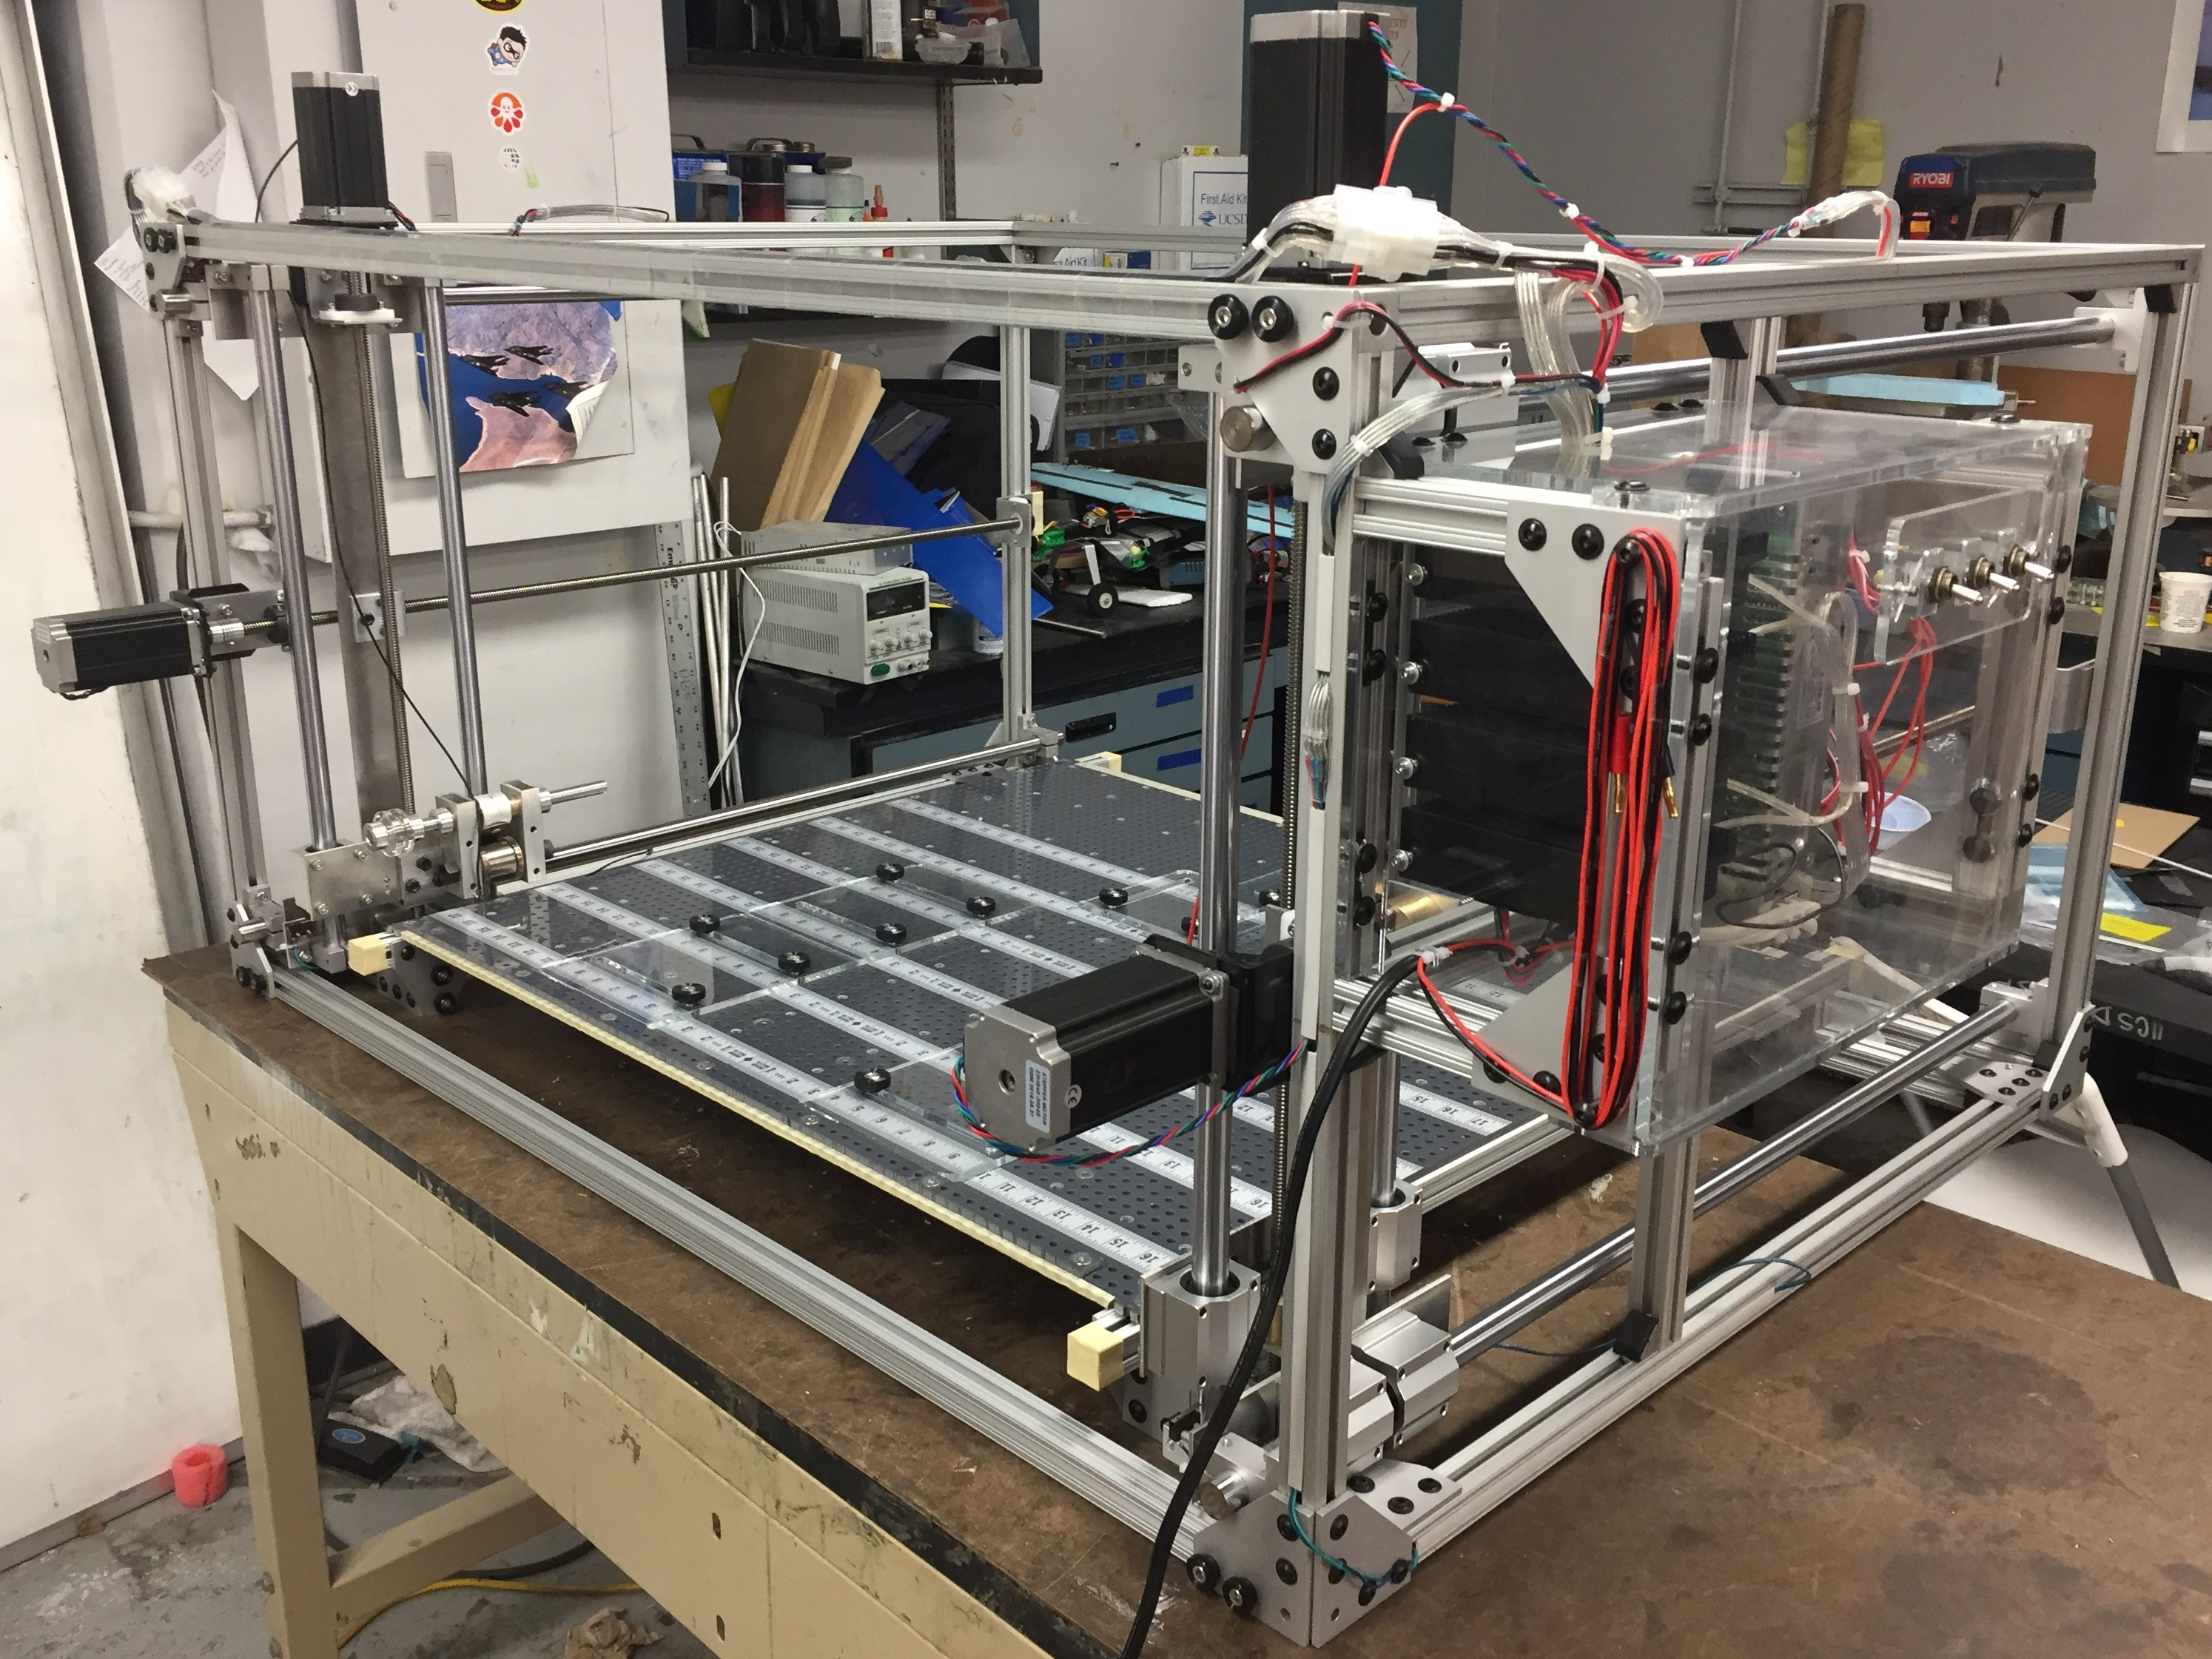
\includegraphics[width = 0.9\linewidth]{./Figures/overview.jpg}
\end{figure}
\begin{figure} [H]
	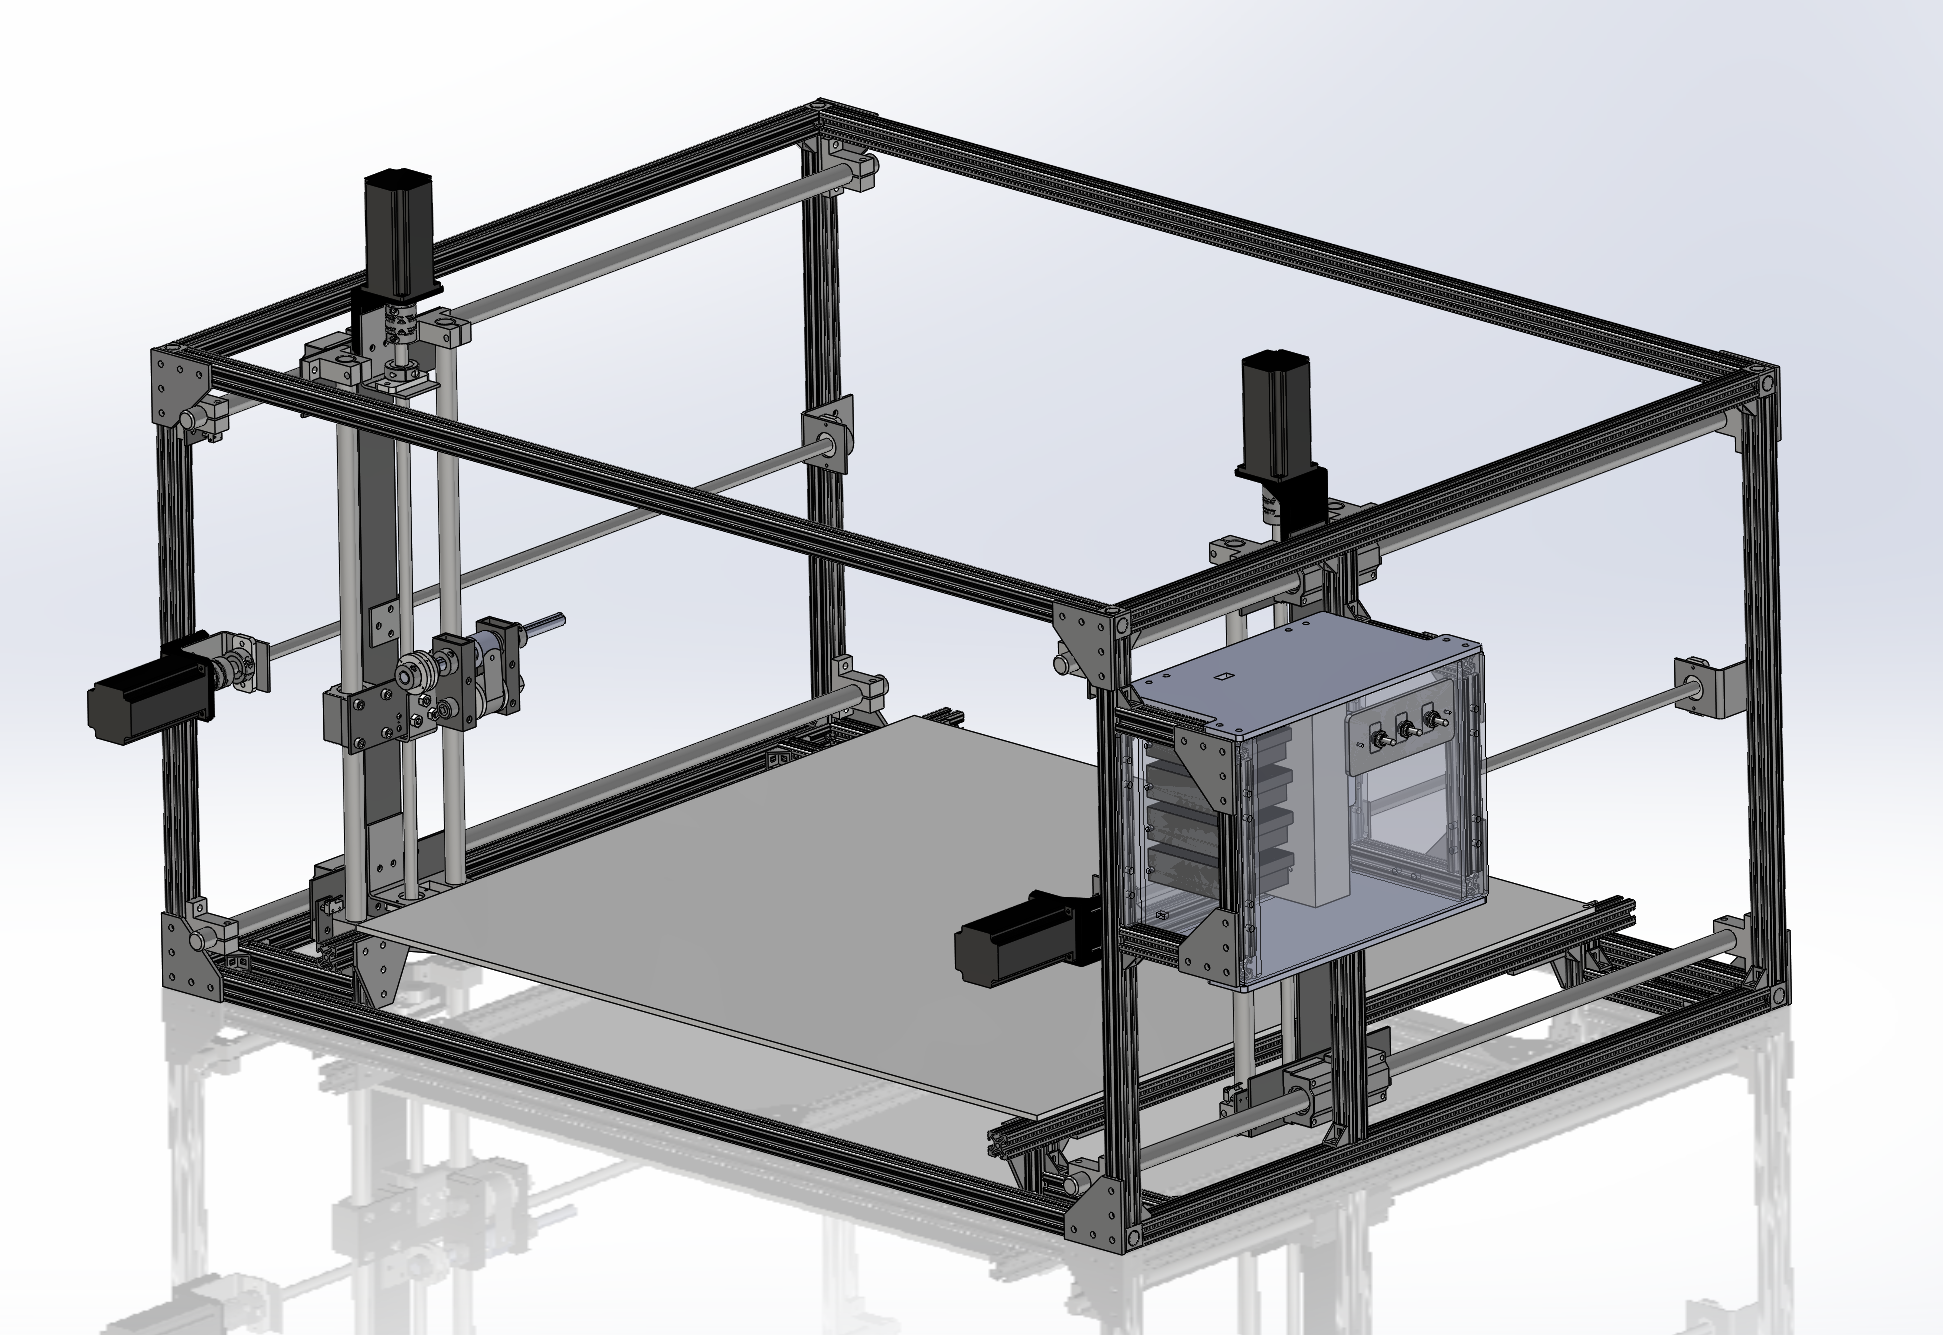
\includegraphics[width = 0.9\linewidth]{./Figures/SW.png}
\end{figure}

\newpage
\tableofcontents
\newpage

\chapter{Preparations}
\section{Laptop Setup} 
\label{sec:laptop}

The foamcutter is controlled by a Raspberry Pi 3 B+. In order to communicate with the Pi, a Windows laptop has to install \textbf{PuTTY} (or similar) to enable secure shell (SSH) connection to the Pi, and \textbf{WinSCP} (or similar) for graphical file management on the Pi. A Linux laptop have SSH capability built in, therefore, no software required. \\

\begin{tcolorbox}
	{\large
		Note:\\ \\
		 This setup process is only required once per laptop. If already performed, skip this section and continue to section~\ref{sec:gcode}.
	}
\end{tcolorbox}

\subsection{PuTTY Setup}

\noindent Please follow the following steps for install and setup of PuTTY:

\begin{enumerate}[itemsep = 5pt,topsep=0pt]
	\item Download PuTTY at \href{https://www.putty.org/}{https://www.putty.org/} then install.
	\item Launch PuTTY and a window similar to fig~\ref{fig:putty1} below should show up:
	\begin{figure} [H]
		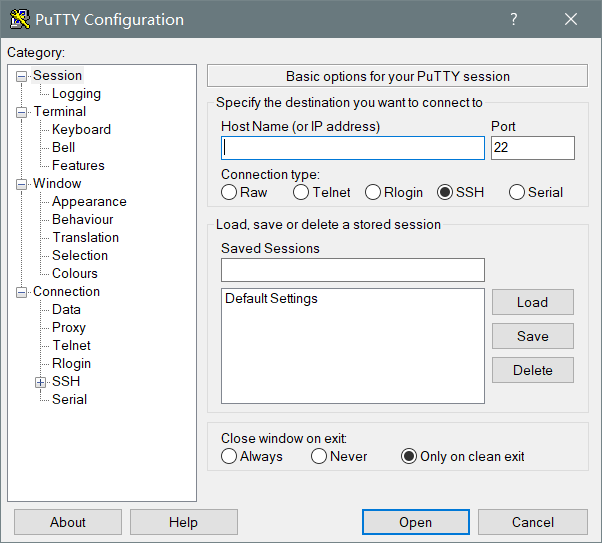
\includegraphics[width = 0.6\linewidth]{./Figures/Laptop_Setup/putty1.png}
		\caption{PuTTY Launch Window}
		\label{fig:putty1}
	\end{figure}
	\item As shown in fig~\ref{fig:putty2} below, in the ``Host Name'' field, enter ``foamcutter.local", then make sure Connection type is SSH. Next, in ``Saved Session field'', enter ``foamcutter", and lastly, click save.
	\begin{figure} [H]
		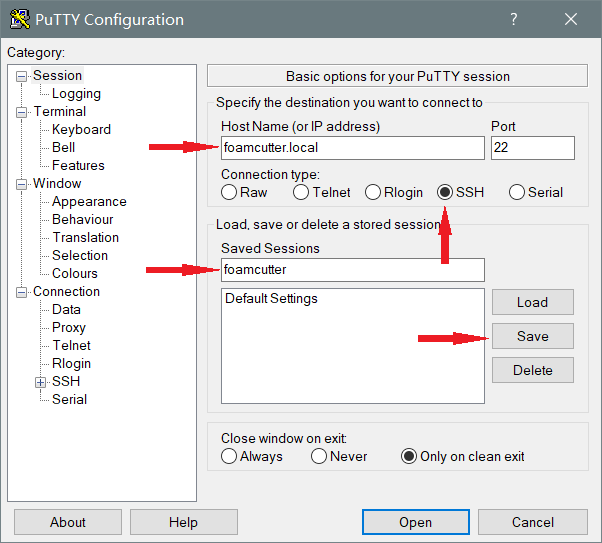
\includegraphics[width = 0.6\linewidth]{./Figures/Laptop_Setup/putty2.png}
		\caption{PuTTY Setup}
		\label{fig:putty2}
	\end{figure}
	\item The session with name ``foamcutter" should show up in Saved Session as shown in fig~\ref{fig:putty3} below, and the PuTTY setup is completed.
	\begin{figure} [H]
		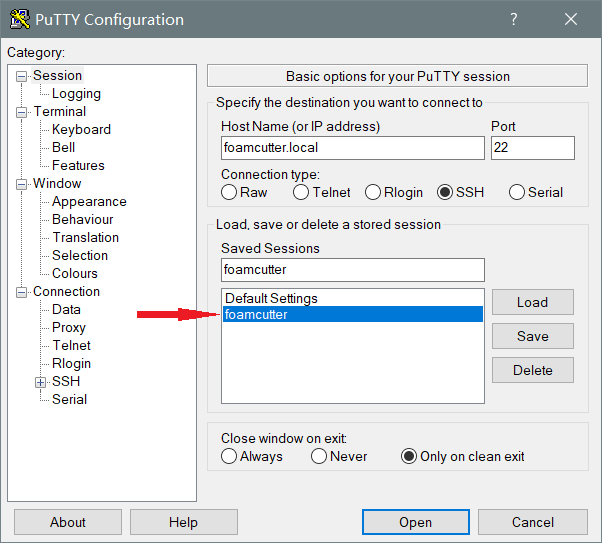
\includegraphics[width = 0.6\linewidth]{./Figures/Laptop_Setup/putty3.png}
		\caption{Saved PuTTY Session}
		\label{fig:putty3}
	\end{figure}
	\item Note on using PuTTY: to copy text from PuTTY, simply select the text, do not press ``Control + C''. To paste text to PuTTY, simply right click mouse, do not press ``Control + V''.
\end{enumerate}

\subsection{WinSCP Setup}

\noindent Please follow the following steps for install and setup of WinSCP:

\begin{enumerate}[itemsep = 5pt,topsep=0pt]
	\item Download WinSCP at \href{https://winscp.net/eng/download.php}{https://winscp.net/eng/download.php} then install.
	\item Launch WinSCP and a window similar to fig~\ref{fig:winscp1} below should show up:
	\begin{figure} [H]
		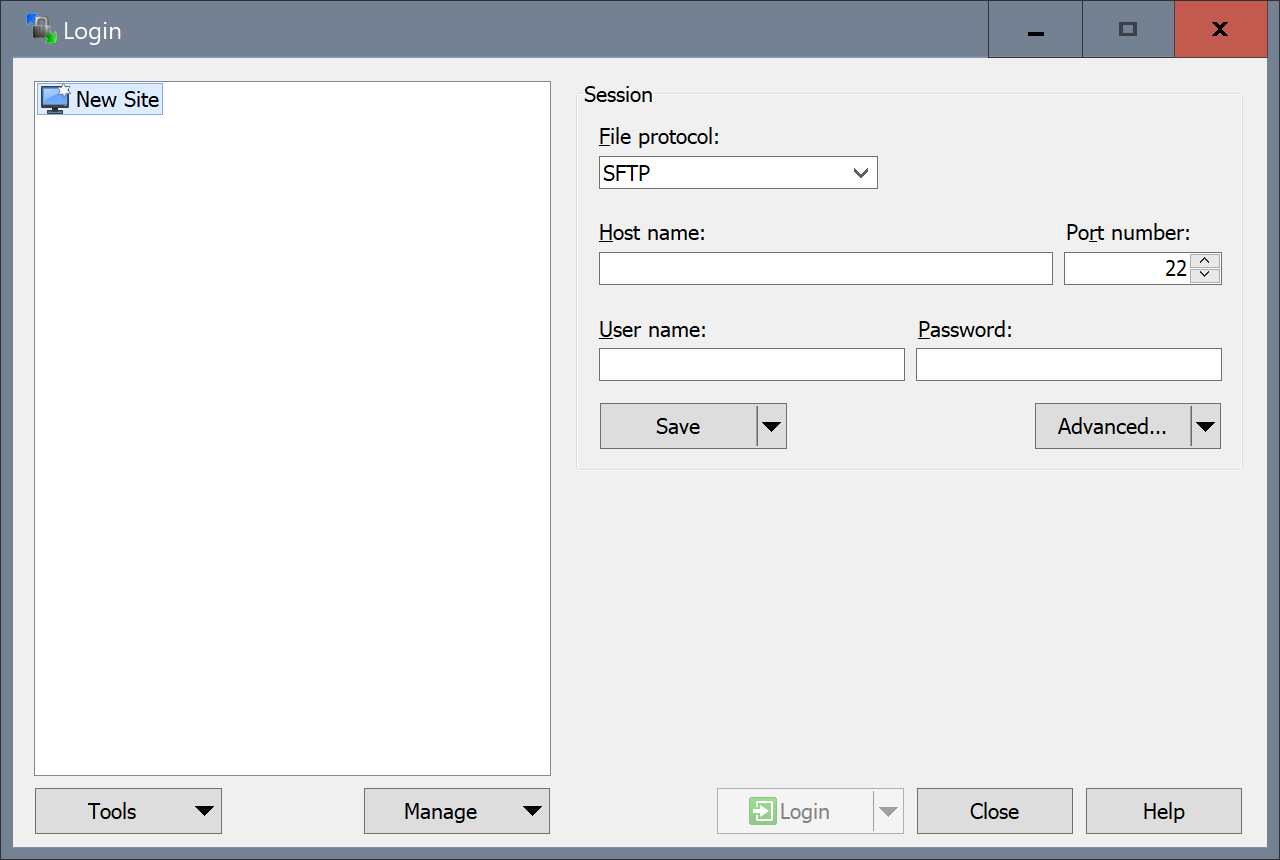
\includegraphics[width = 0.6\linewidth]{./Figures/Laptop_Setup/winscp1.png}
		\caption{WinSCP Launch Window}
		\label{fig:winscp1}
	\end{figure}
	\item As shown in fig~\ref{fig:winscp2} below, make sure the protocol is ``SFTP", then enter ``foamcutter.local" for the host name, ``pi" for the user name, and ``ucsdaiaadbf" for the password.
	\begin{figure} [H]
		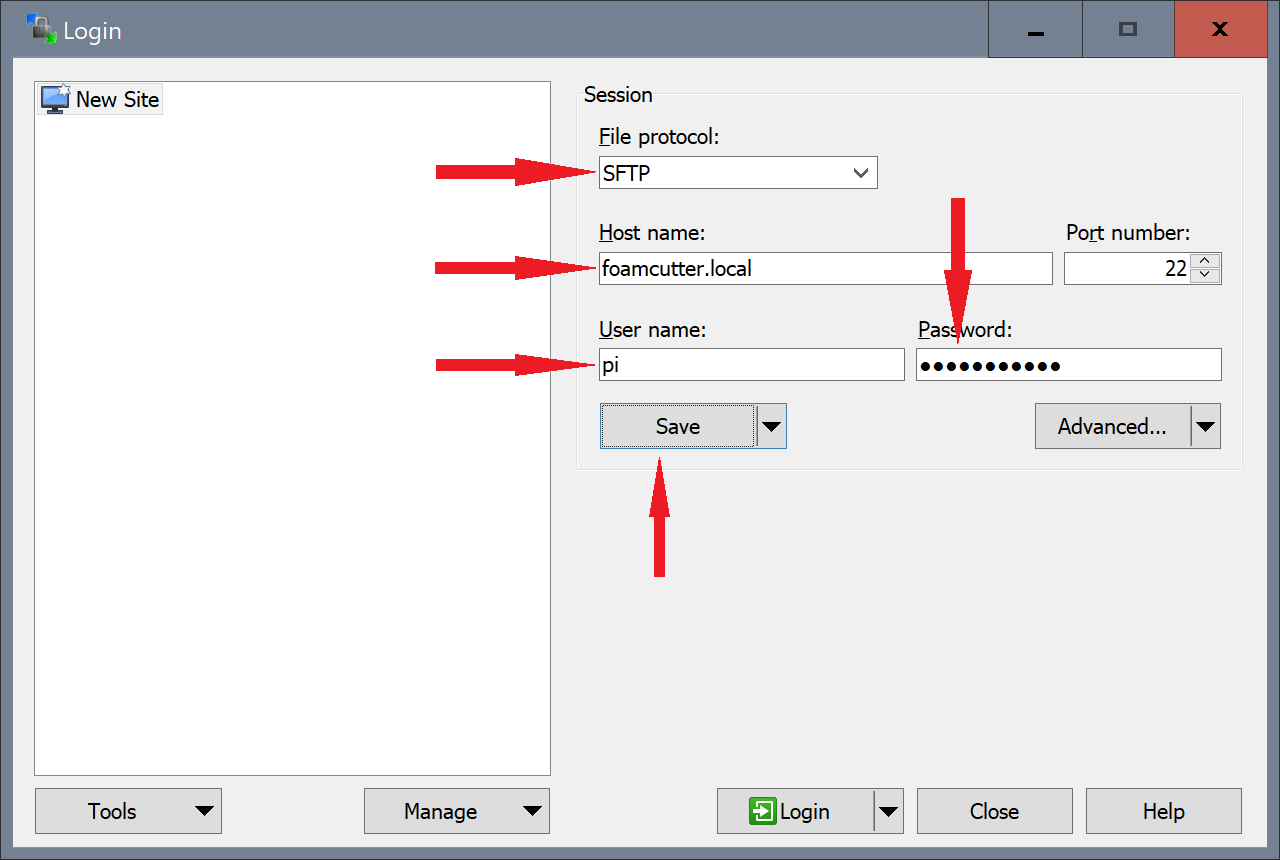
\includegraphics[width = 0.6\linewidth]{./Figures/Laptop_Setup/winscp2.png}
		\caption{WinSCP Setup}
		\label{fig:winscp2}
	\end{figure}
	\item Click save, and a window shown in fig~\ref{fig:winscp3} below should pop up. Both ``Save password" and ``Create desktop shortcut" are recommended. Click ``OK" and the setup for WinSCP is completed. 
	\begin{figure} [H]
		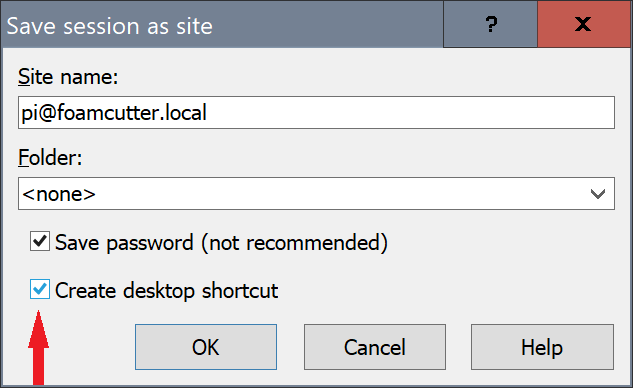
\includegraphics[width = 0.6\linewidth]{./Figures/Laptop_Setup/winscp3.png}
		\caption{WinSCP Setup continued}
		\label{fig:winscp3}
	\end{figure}
\end{enumerate}


\subsection{Install Bonjour Print Service}
Download and install Bonjour Print Service from \href{https://support.apple.com/kb/DL999?locale=en_US}, this will enable PuTTY to ssh into the pi with its hostname. 

\newpage



\section{Assemble the Foamcutter}
\label{sec:assemble}

The entire foamcutter as shown in fig~\ref{fig:overview} below consists of two side frames each having two axis of motion, four 4-feet long connection rods, and a work panel for securing the foam. 

\begin{figure} [H]
	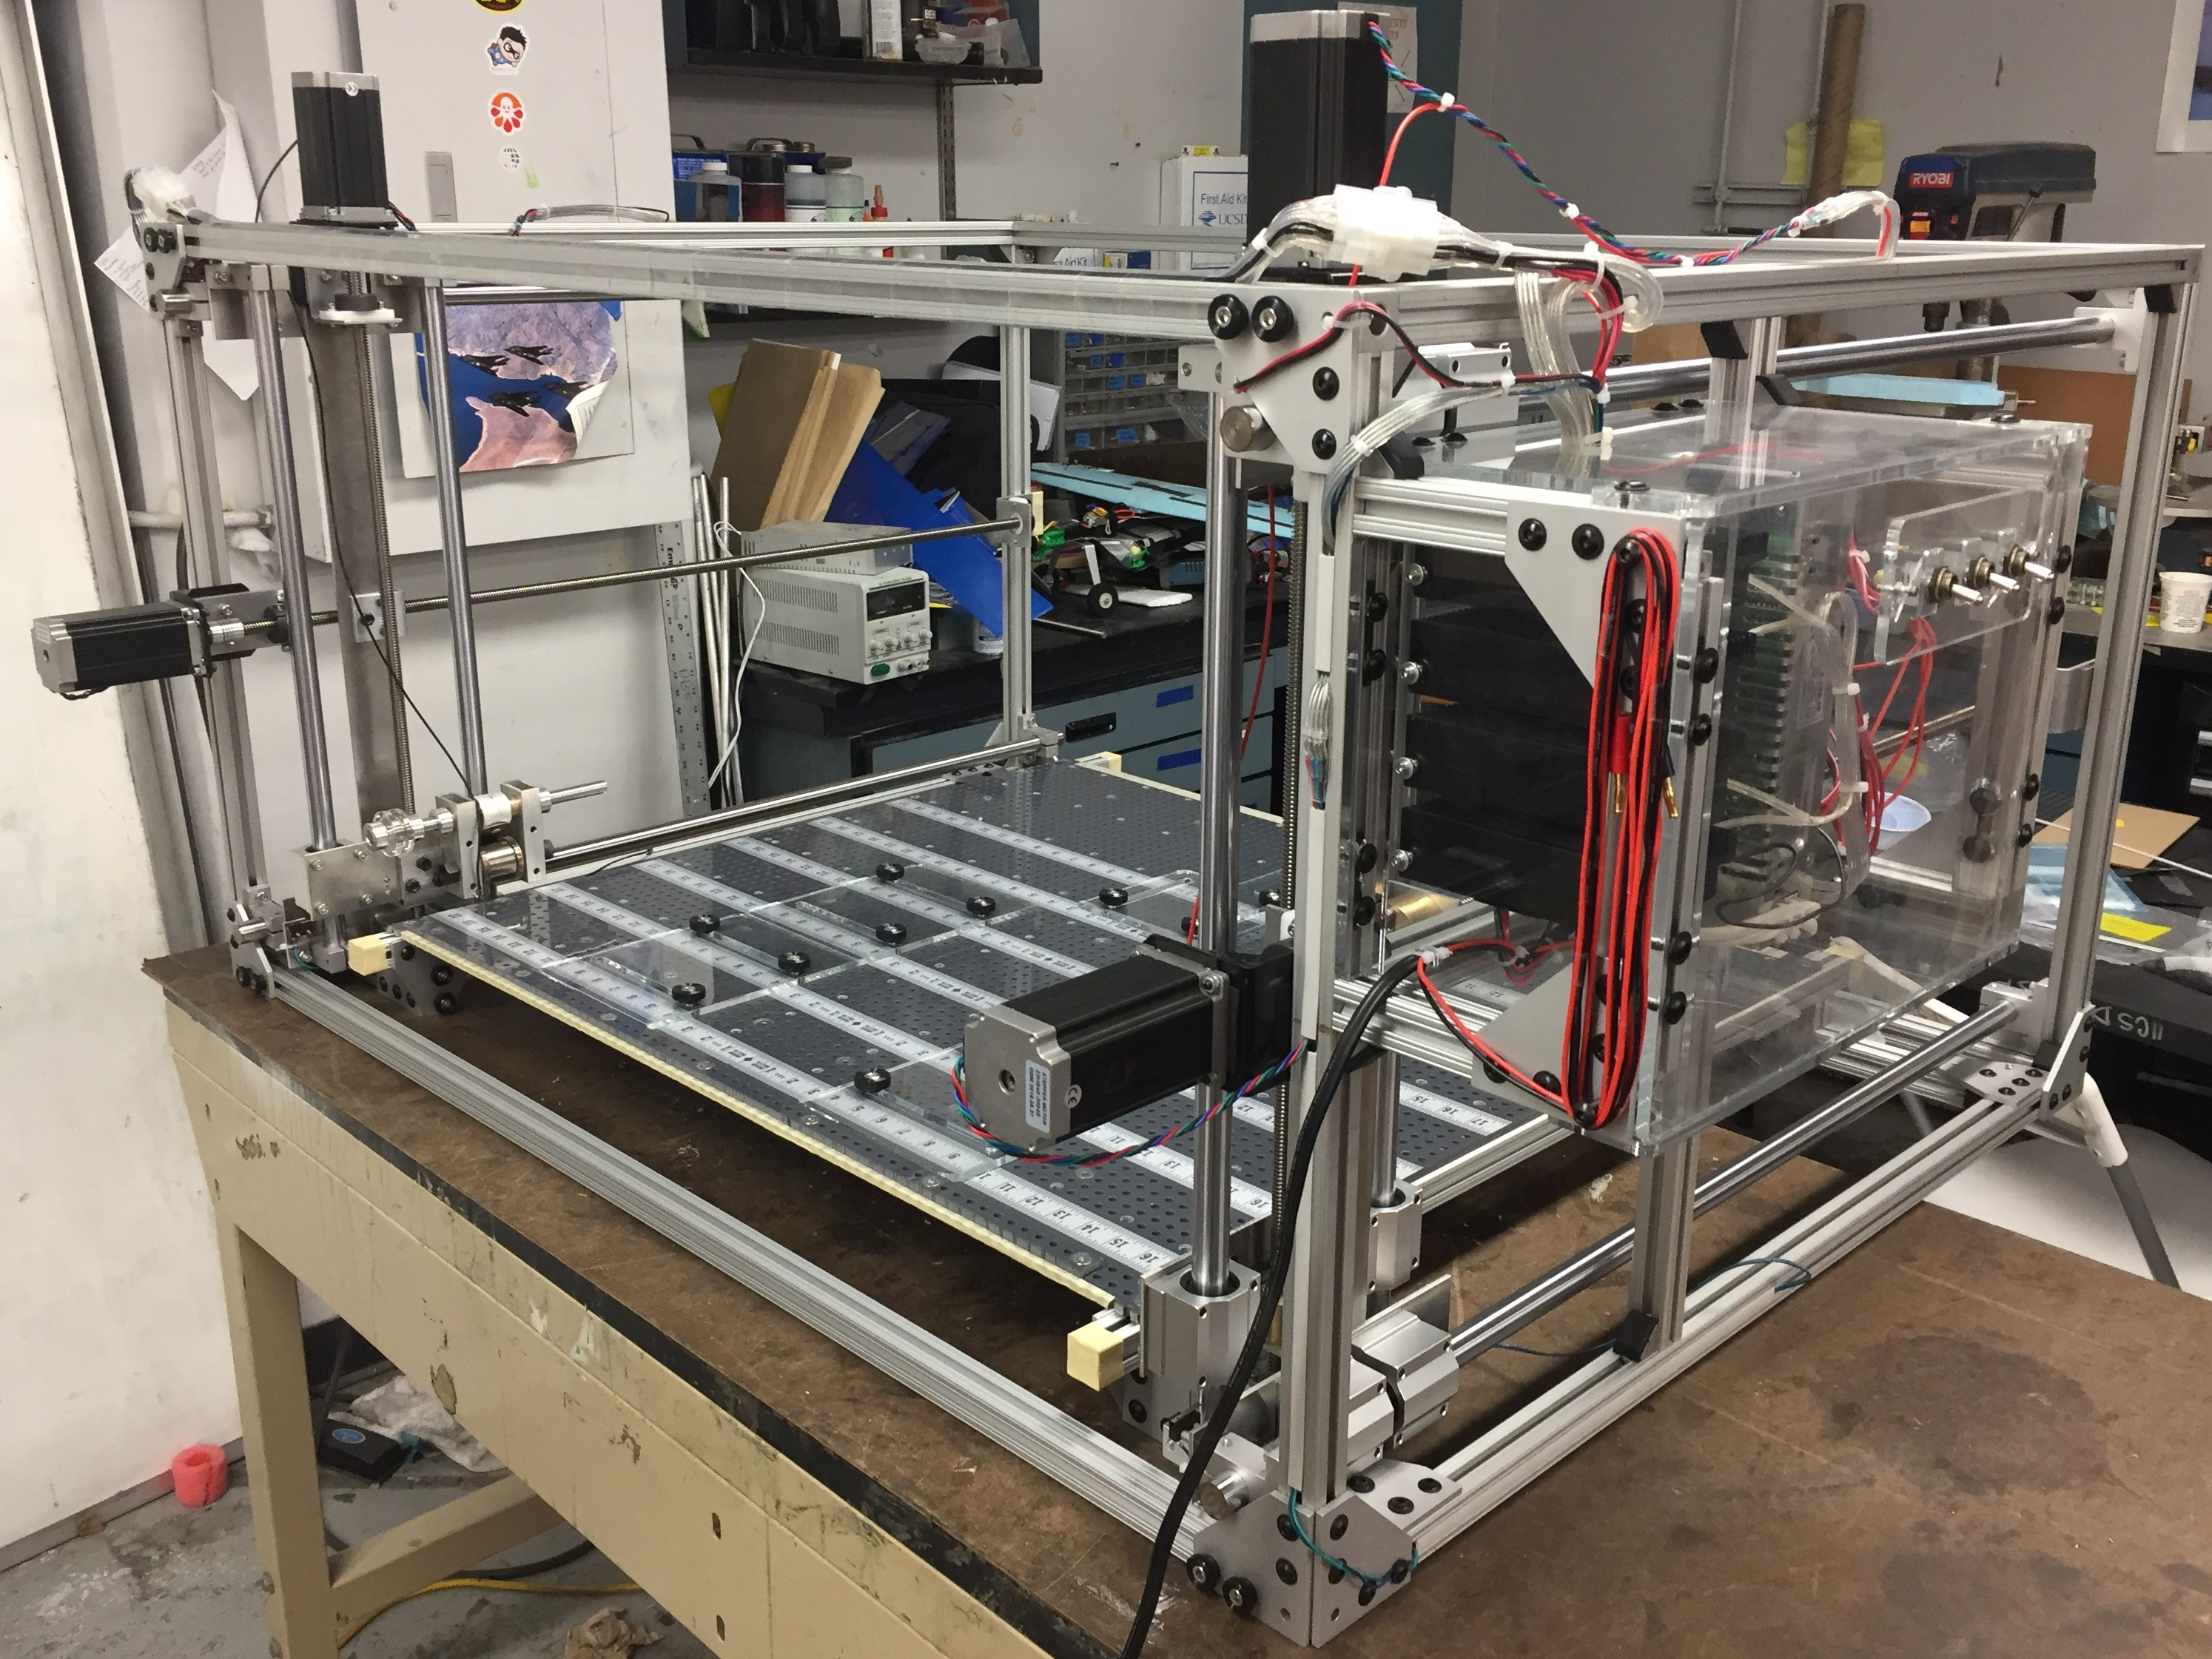
\includegraphics[width = 0.9\linewidth]{./Figures/overview.jpg}
	\caption{Foamcutter Overview}
	\label{fig:overview}
\end{figure}

\begin{tcolorbox}
	{\large
		\noindent Caution:
		\begin{itemize}[noitemsep,topsep=0pt]
			\item Side frames are extremely heavy, lift with caution;
			\item Avoid bumping head onto the connection rods when leaning into and out of the frame.
		\end{itemize}
	}
\end{tcolorbox}

\begin{tcolorbox}
	{\large
\noindent Do:
\begin{itemize}[noitemsep,topsep=0pt]
	\item Always make sure the two side frames are connected with the connection rods;
	\item Always push the two side frames firmly against each other before tightening the thumb screws;
	\item Remember to plug in the two Molex connectors.
\end{itemize}

\noindent Don't:
\begin{itemize}[noitemsep,topsep=0pt]
	\item Never let the side frames stand on their own;
	\item Never over tighten the thumb screws on the work panel;
	\item Never unscrew screws that are not thumb screws unless performing repairs.
\end{itemize}
}
\end{tcolorbox}

\subsection{Connect the two Side Frames}
The two side frames are connected with 4 connection rods, use the 4ft long connection rods for performing cutting and use the 2ft long connection rods (not purchased yet) for storage of the foamcutter. Each of the 4 connection rods are secured with two thumb screws at each end shown in fig~\ref{fig:thumb_screw}, loosen the thumb screws to remove the connection rod. 

\begin{figure} [H]
	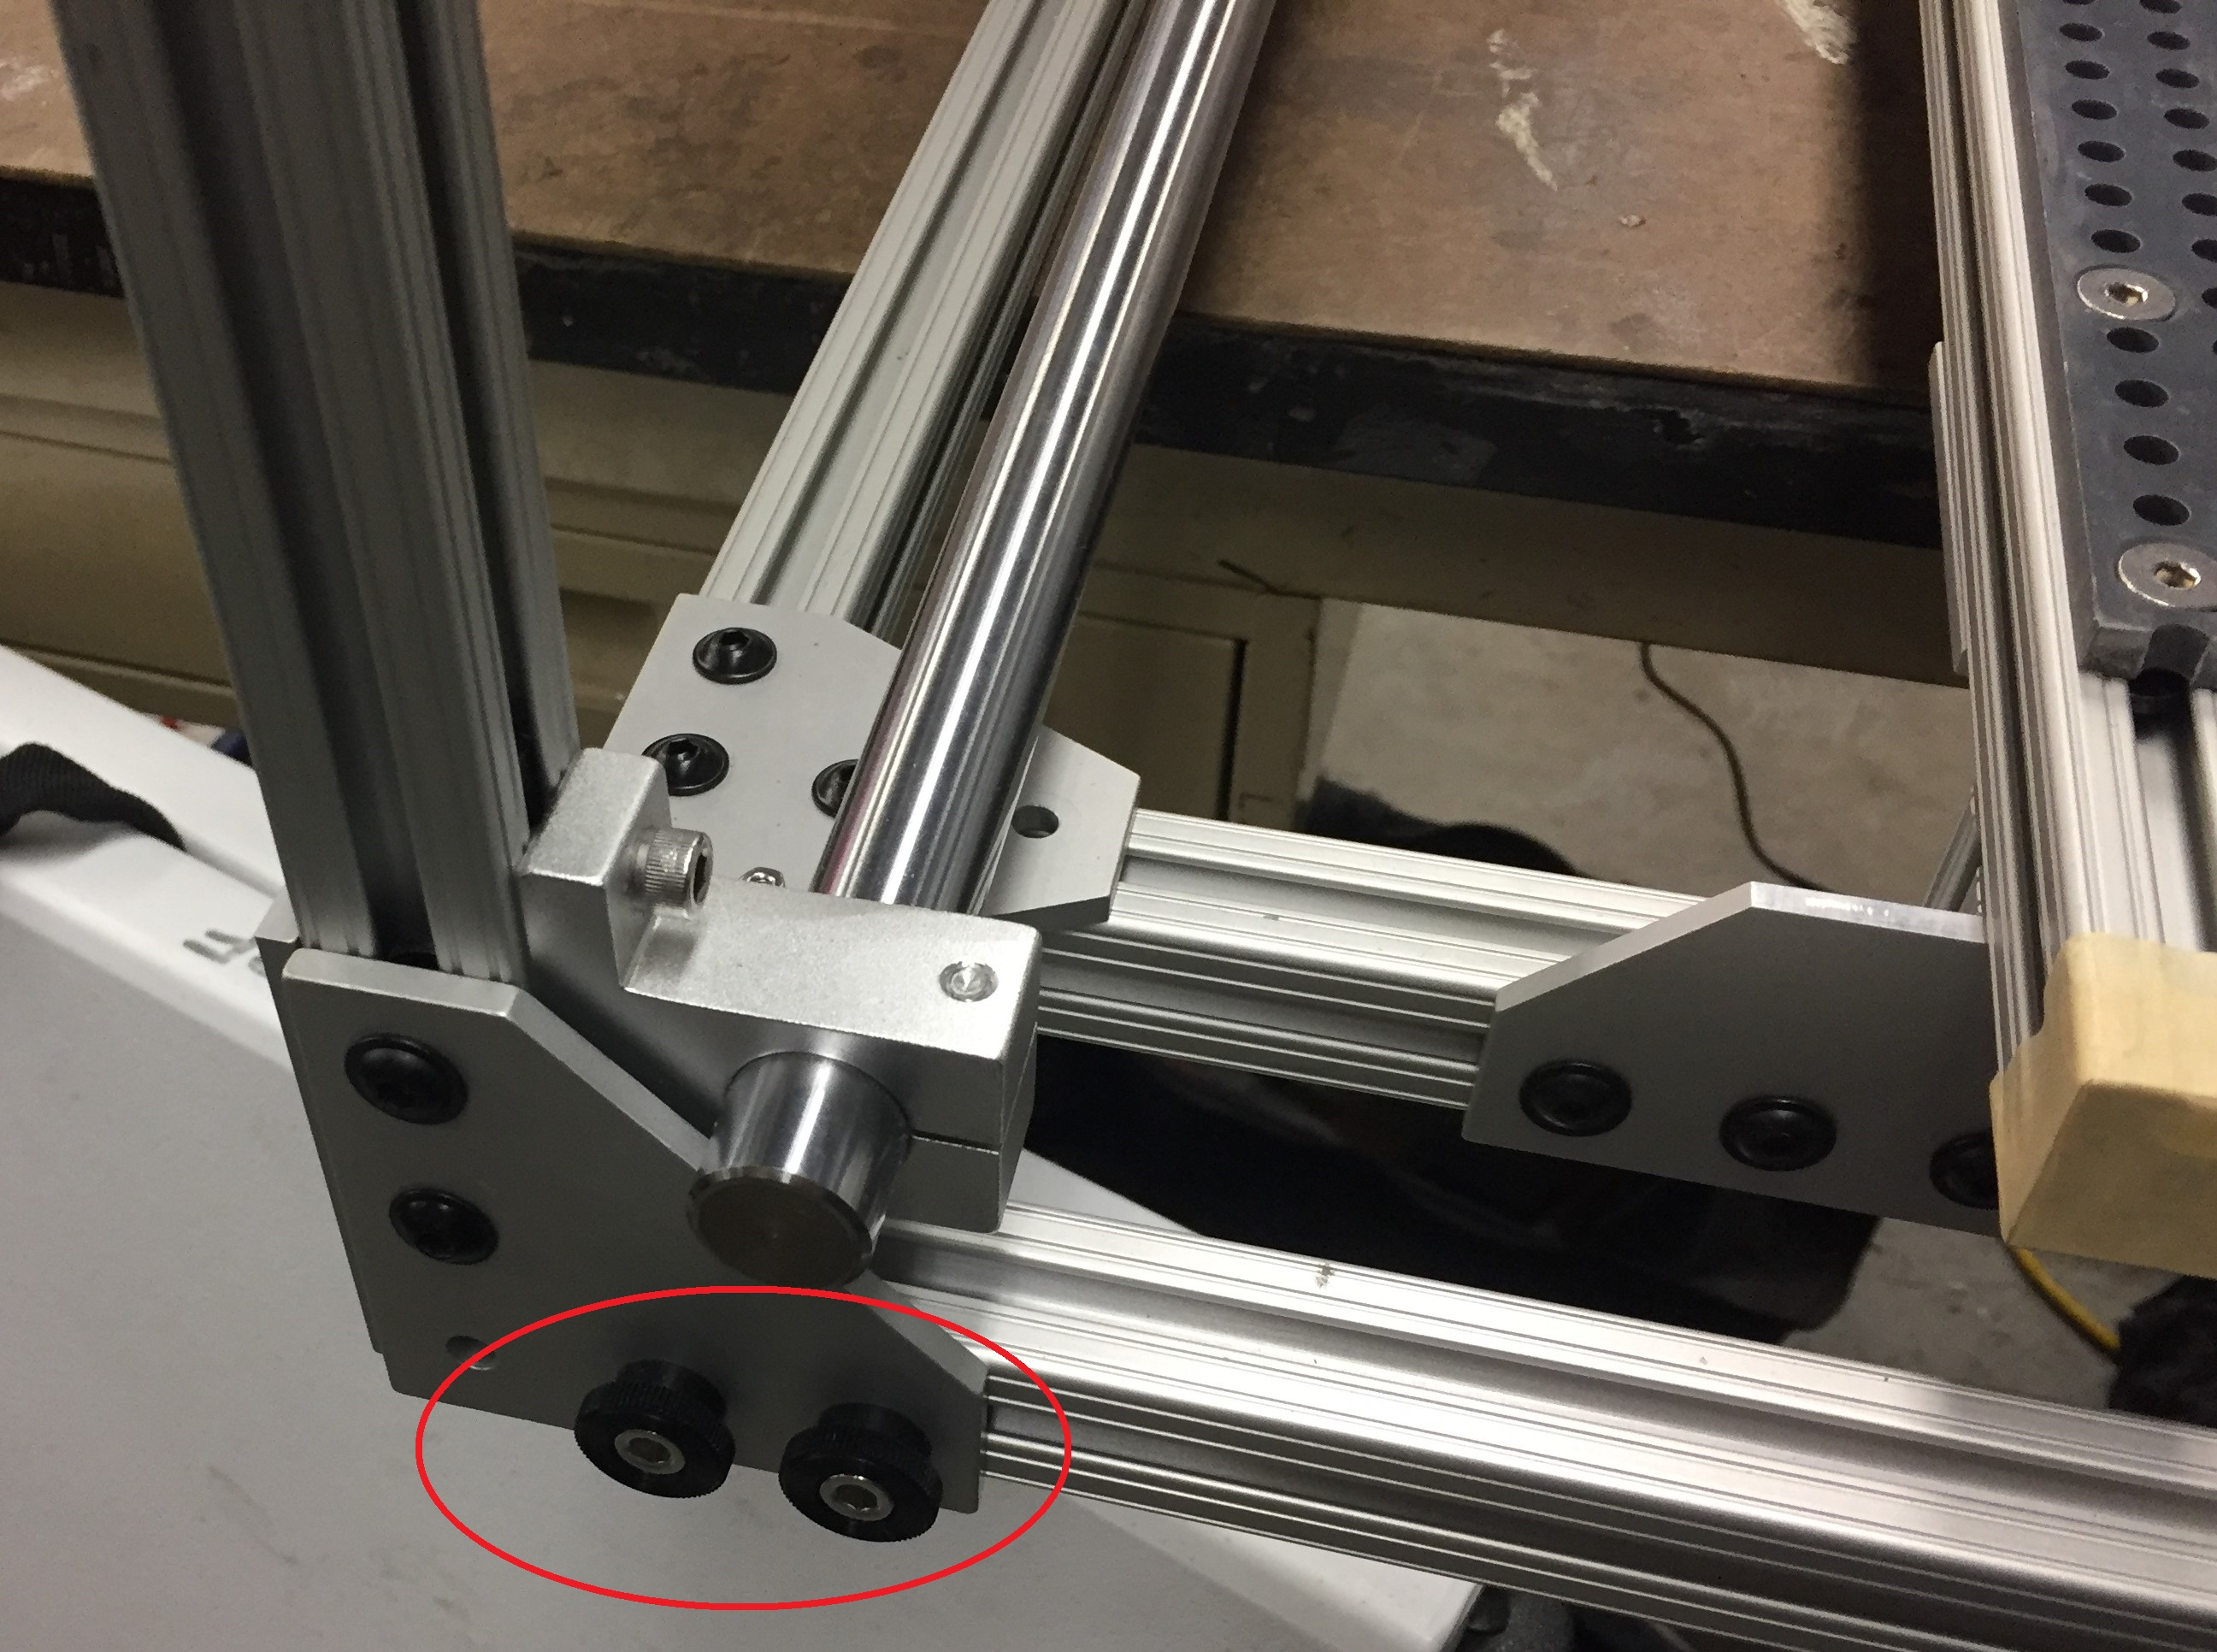
\includegraphics[width = 0.8\linewidth]{./Figures/thumb_screw.jpg}
	\caption{Thumb Screws for Connection Rods}
	\label{fig:thumb_screw}
\end{figure}

During the installation of the connection rods, do not let the side frames stand on their own. The side frames are capable of standing on their own, but are not designed to do so: deformation will occur and degrade the accuracy. When installing the connection rods, push the two side frames firmly against each other to make sure there are no gaps between the side frames and the connection rods. Then tighten the thumb screws. An Allen key is recommended to further tighten the thumb screws.

\subsection{Connect two Molex Connector}

There are two Molex connectors located at the two top corners of the foamcutter as shown in fig~\ref{fig:molex} below. Make sure to connect them before operating the foamcutter. The Molex connectors are foolproof, \textbf{do not force it when unable to plug in}.


\begin{figure}[H]
	\centering
	\begin{minipage}[b]{0.603 \linewidth}
		{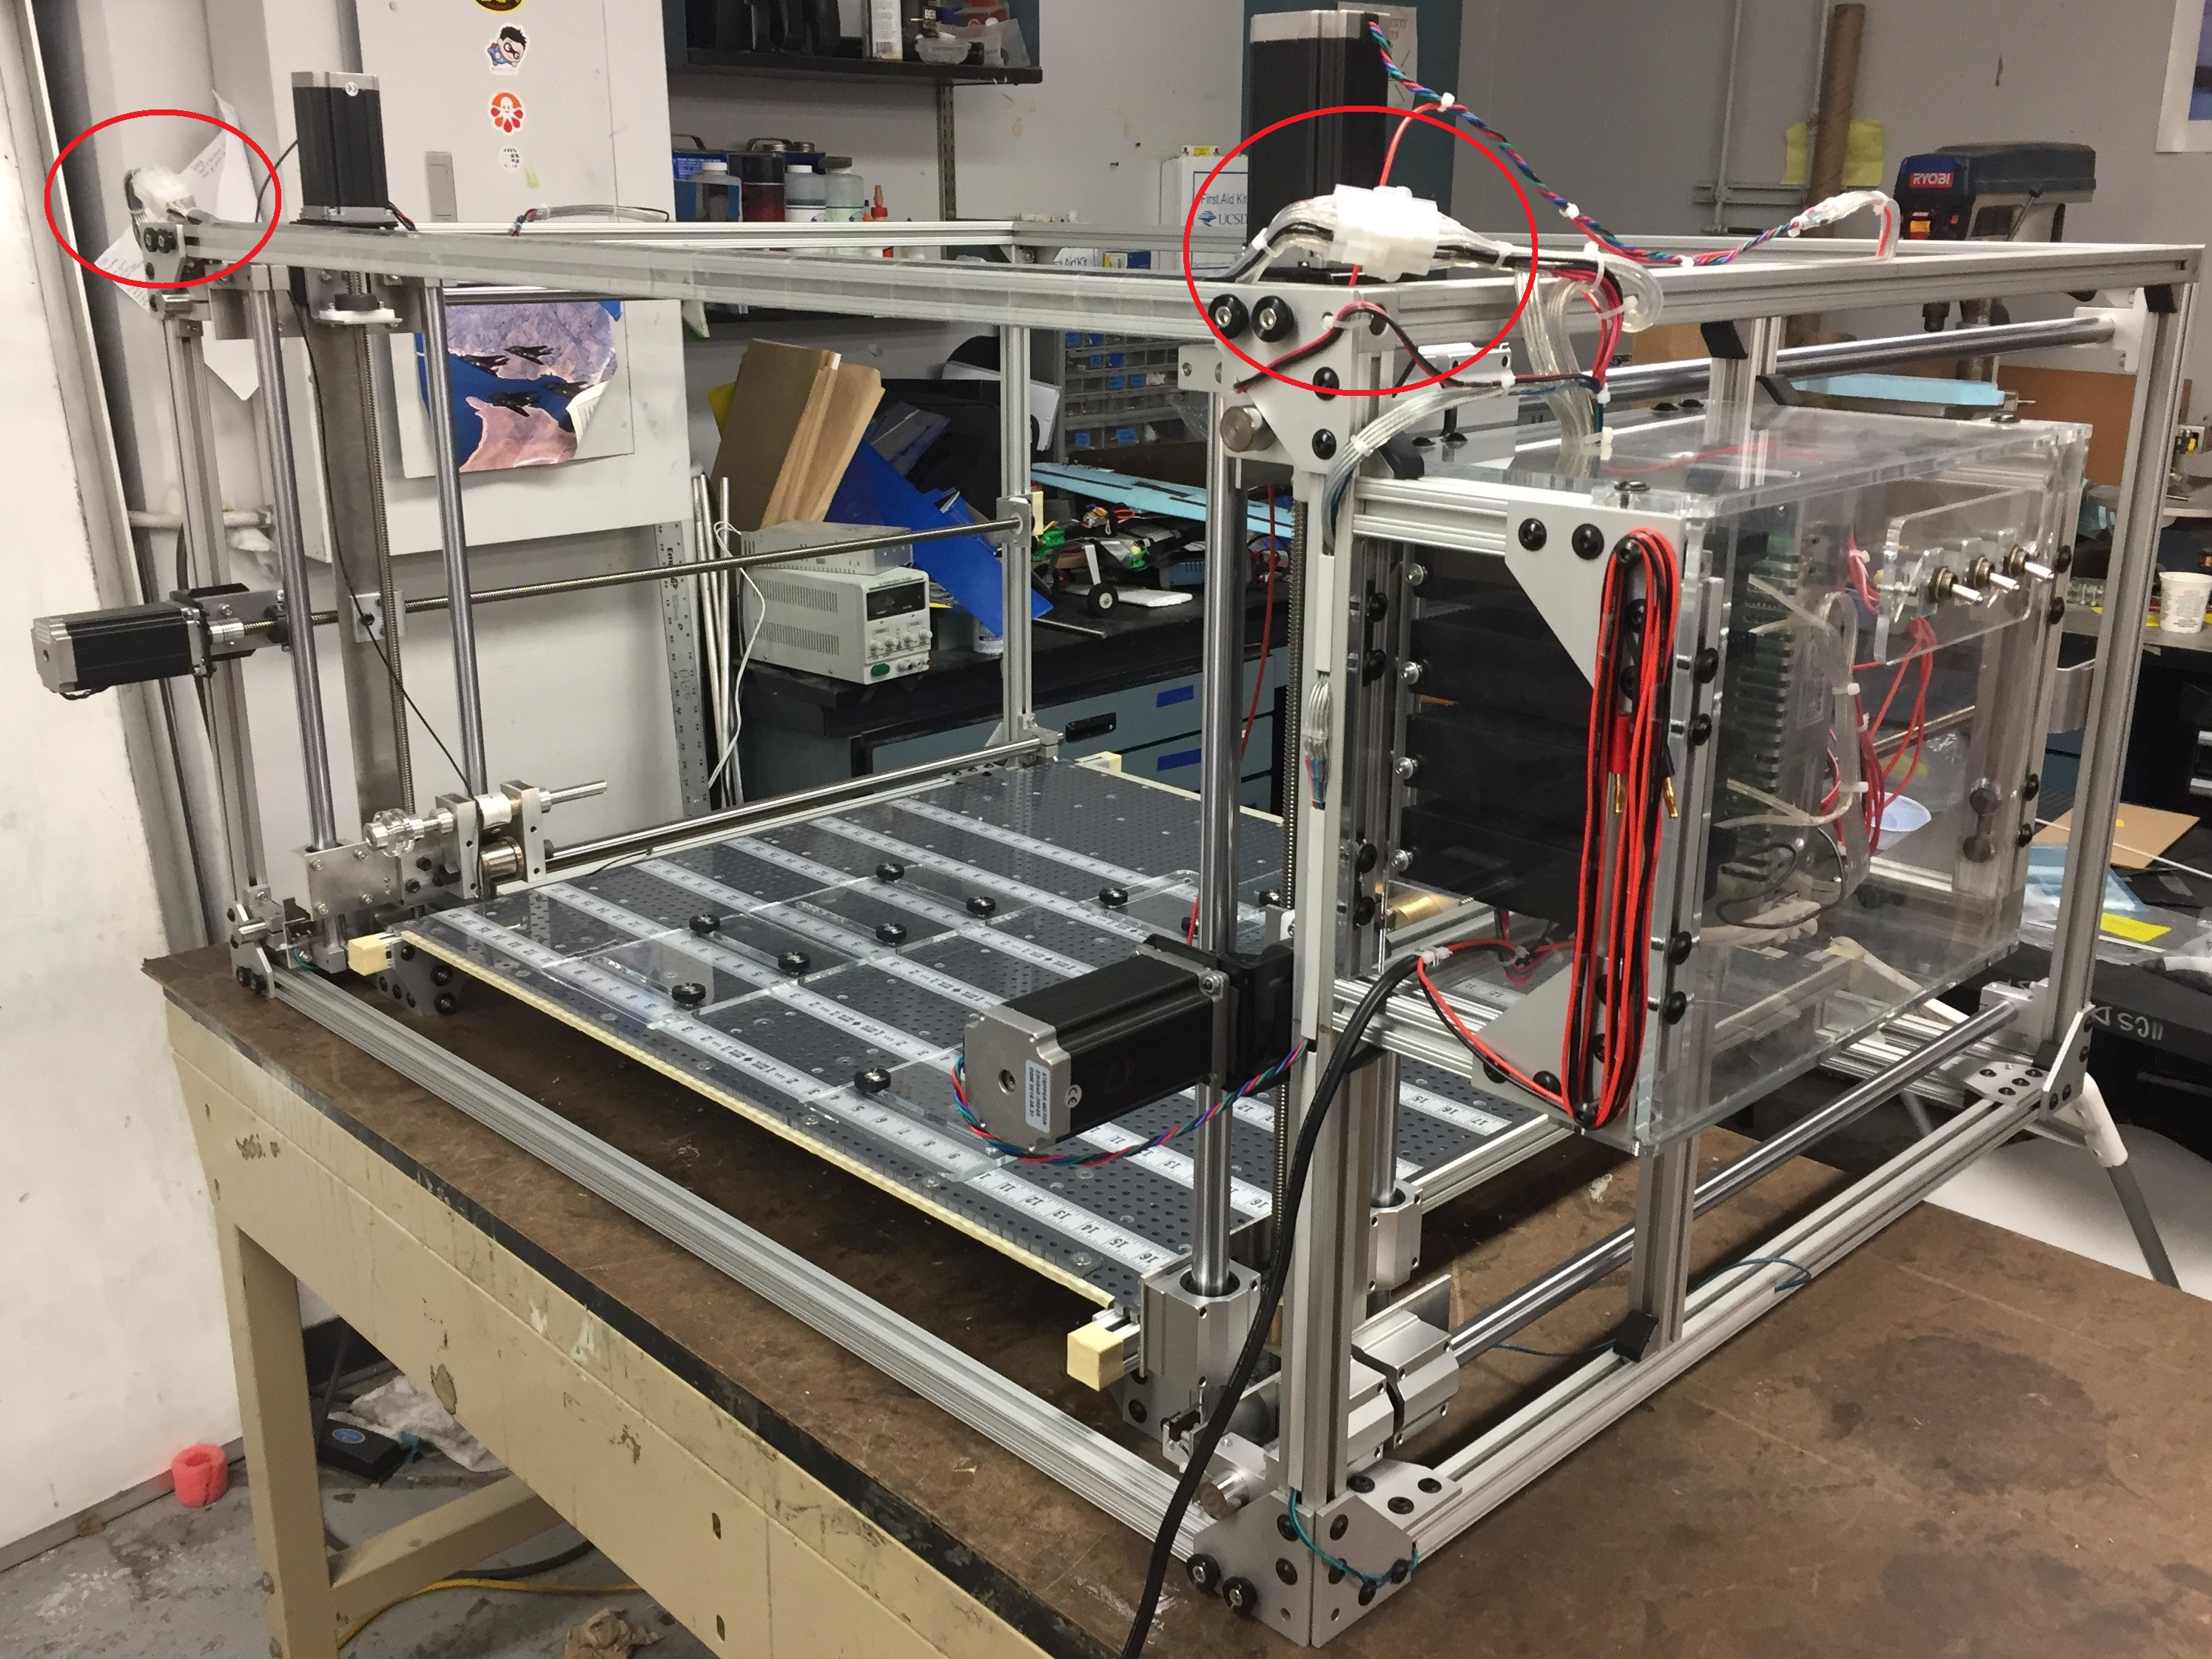
\includegraphics[width=\textwidth]{./Figures/molex.jpg}}
	\end{minipage}
	\begin{minipage}[b]{0.3 \linewidth}
		{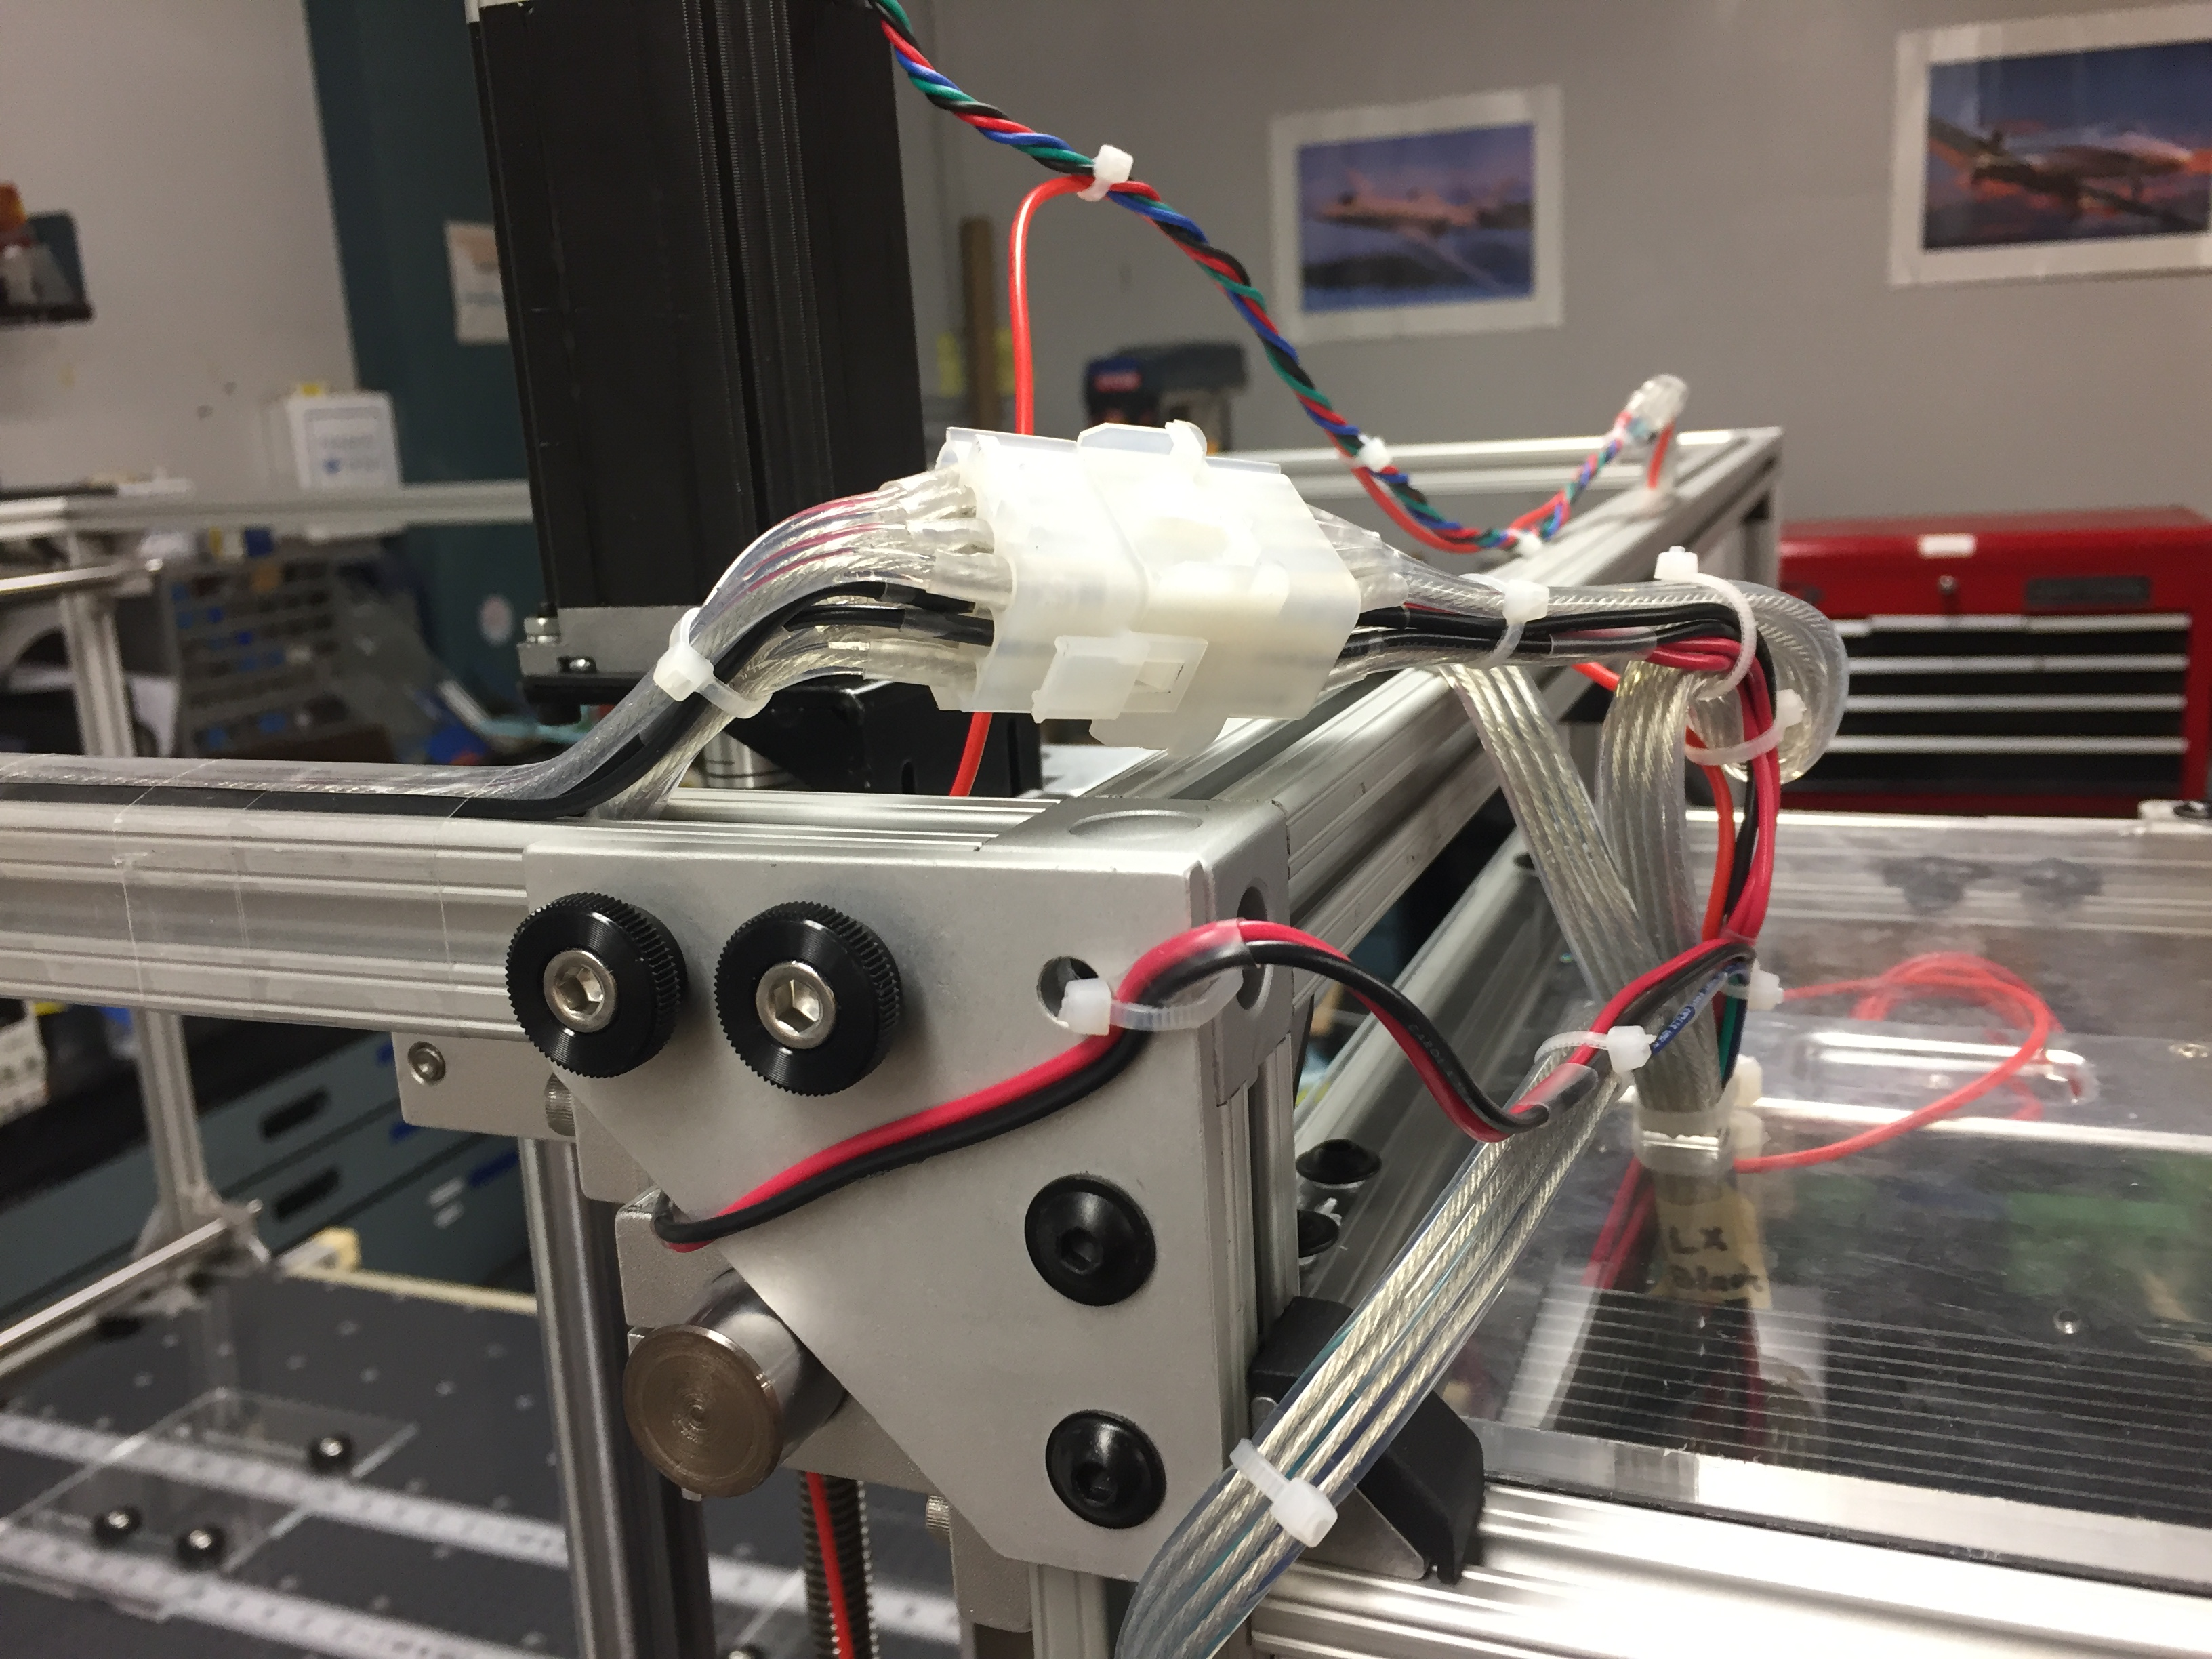
\includegraphics[width=\textwidth]{./Figures/molex1.jpg}}
		\vfill
		{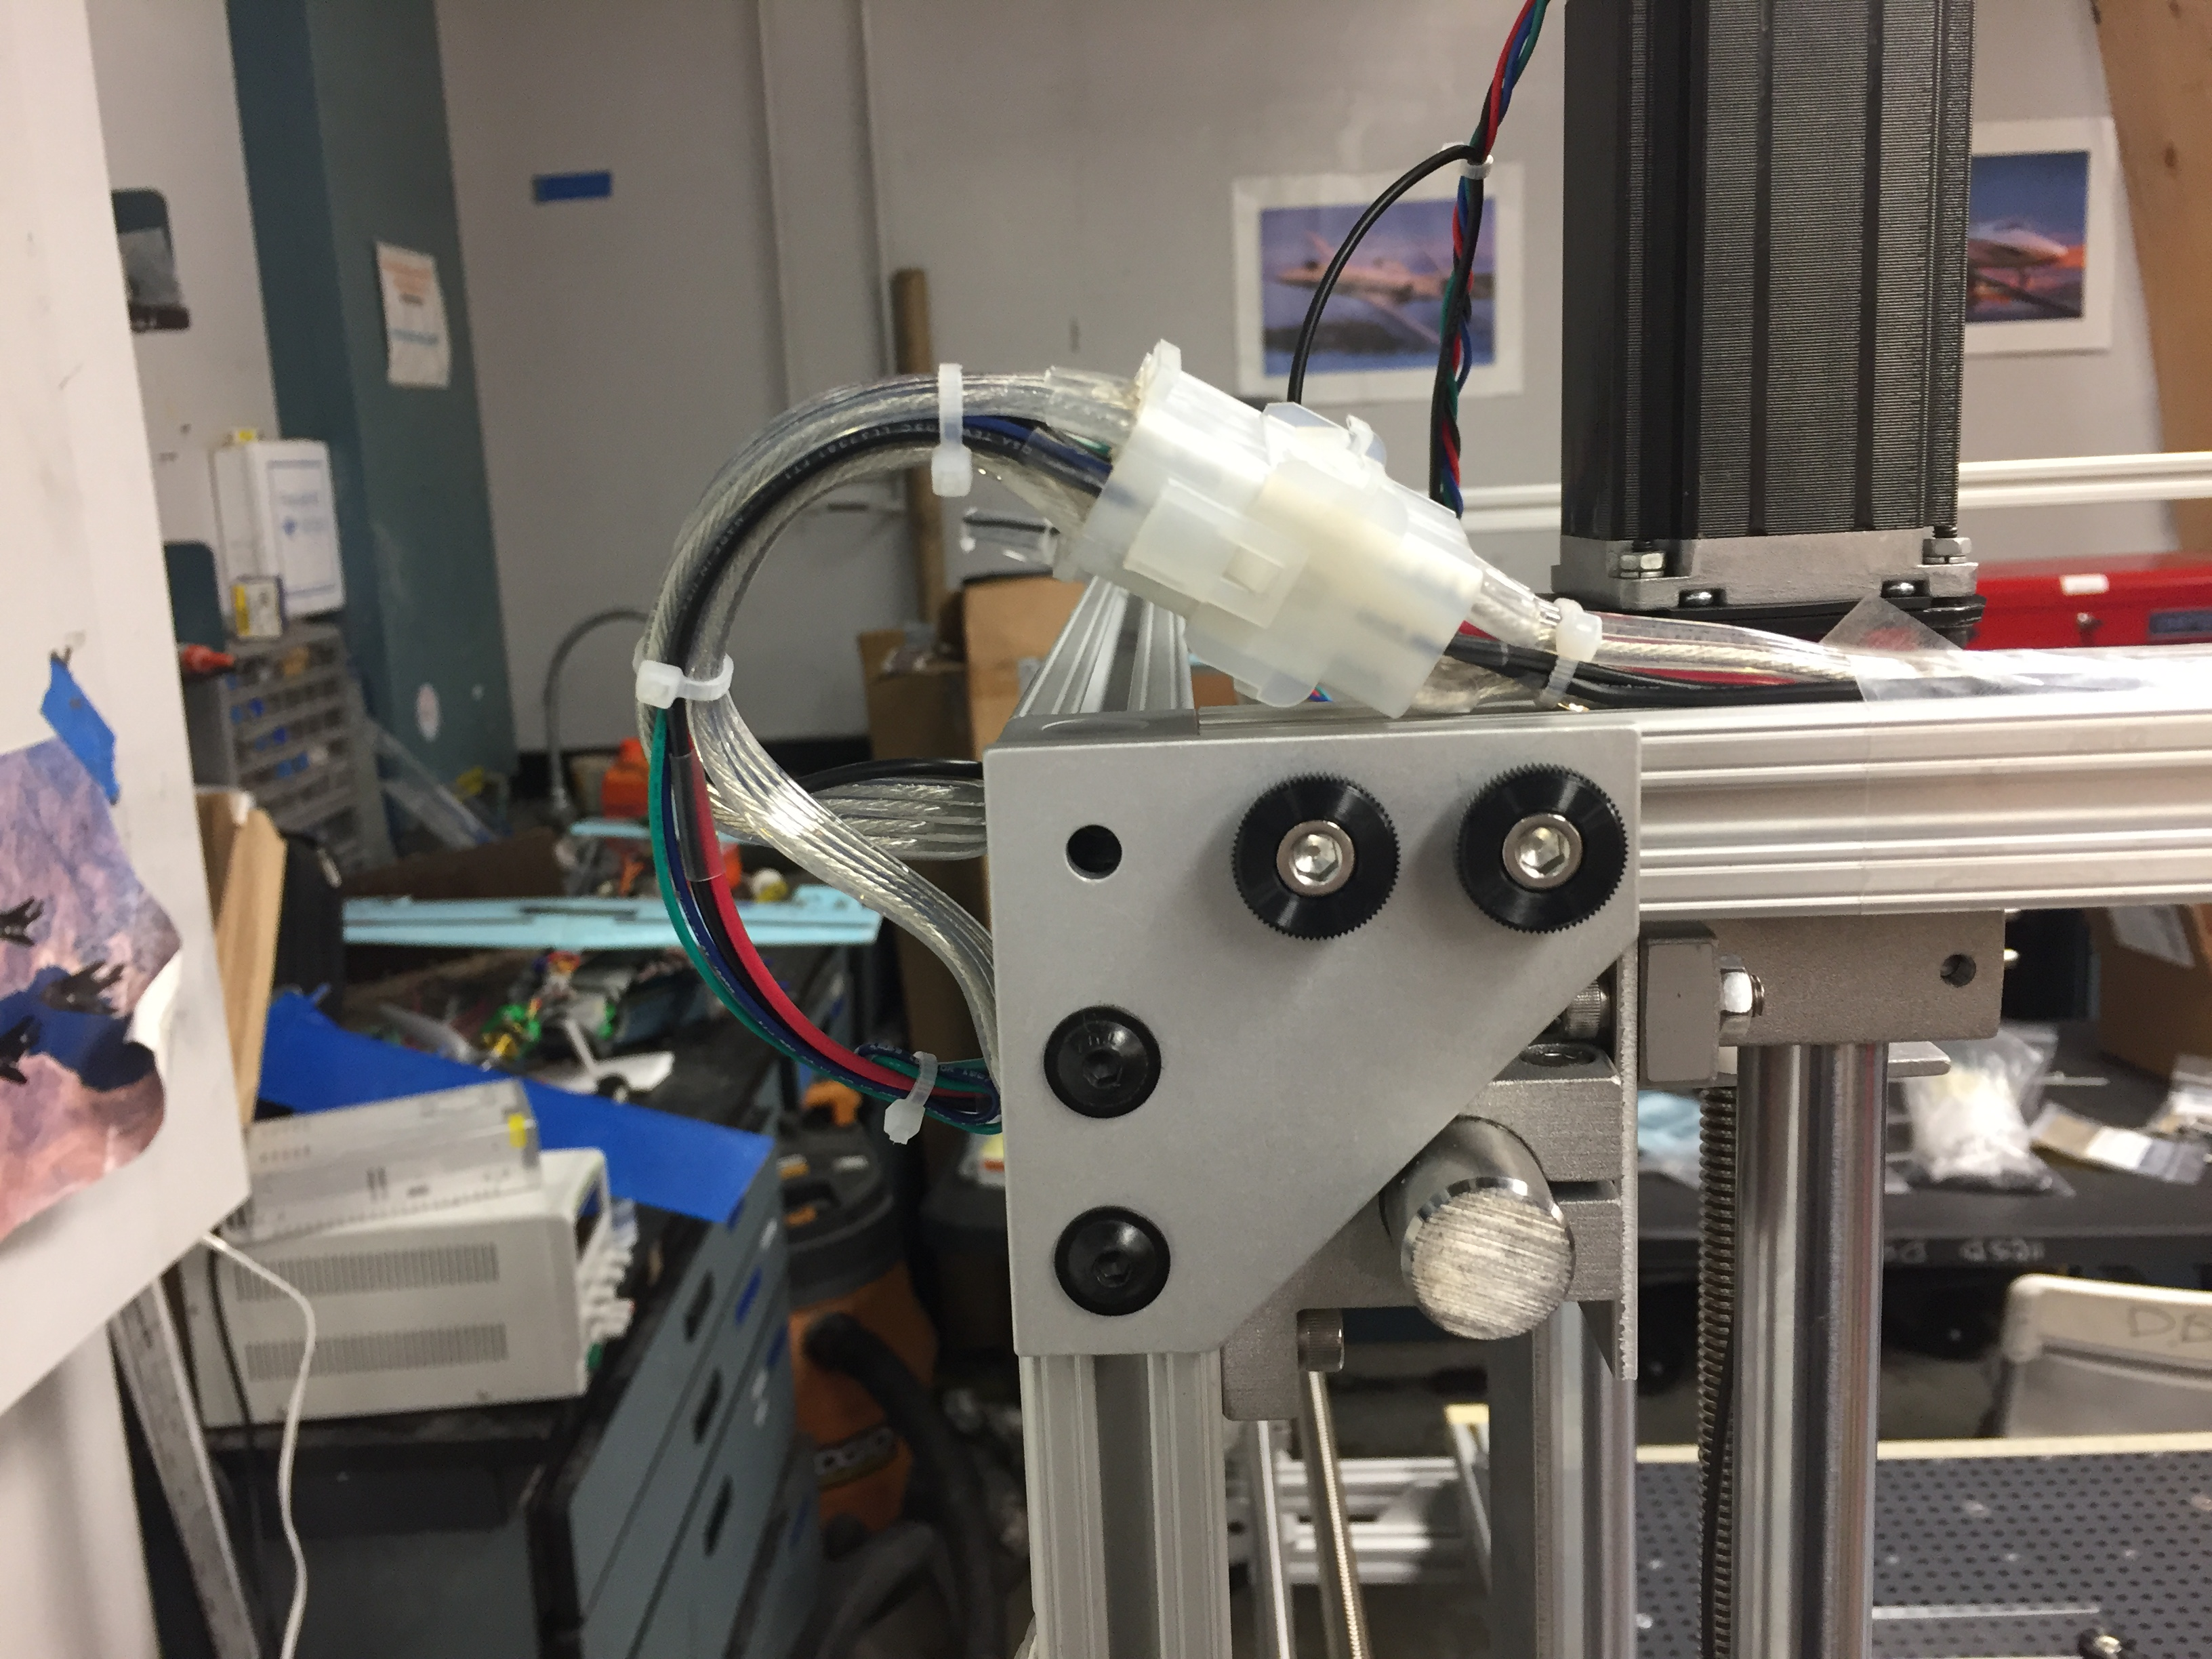
\includegraphics[width=\textwidth]{./Figures/molex2.jpg}}
	\end{minipage}
	\caption{Molex Connectors}
	\label{fig:molex}
\end{figure}

\subsection{Install the Work Panel}
The work panel is connected to the two side frames at the four corners of the panel. Each corner is secured with two thumb screws as shown in fig~\ref{fig:panel} below. 
\begin{figure} [H]
	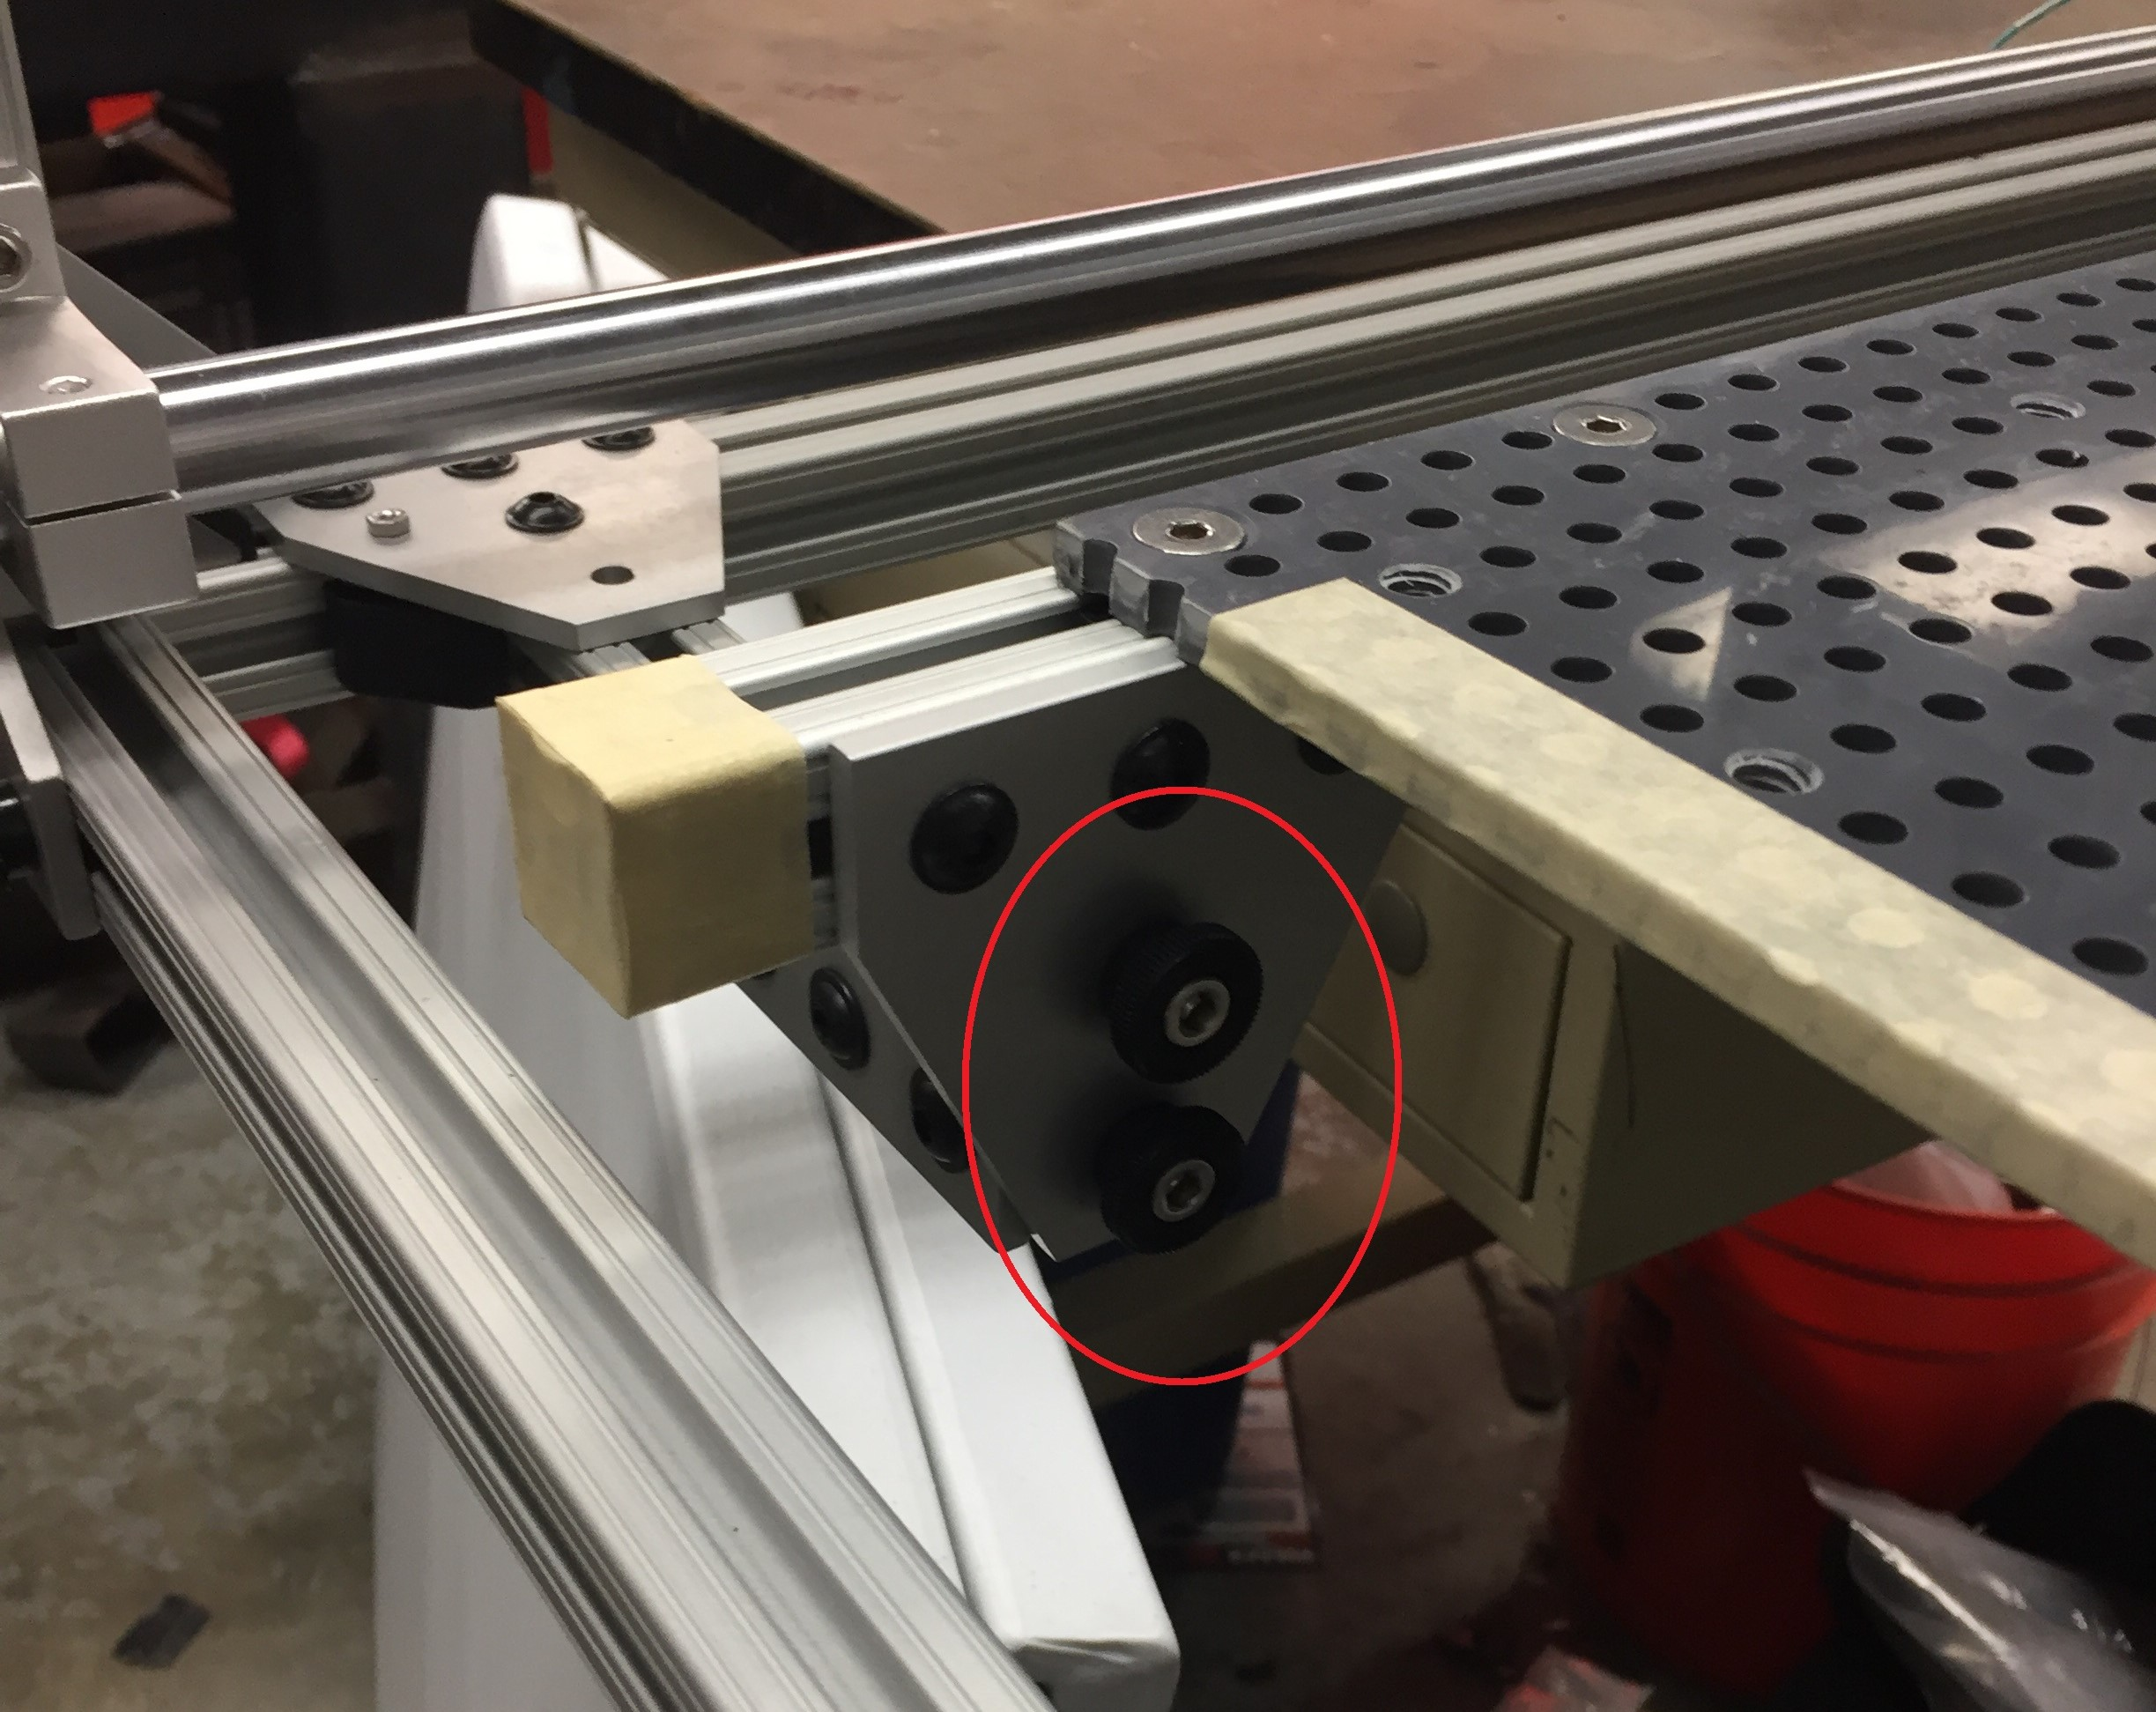
\includegraphics[width = 0.8\linewidth]{./Figures/panel_thumb_screw.jpg}
	\caption{Work Panel Thumb Screws}
	\label{fig:panel}
\end{figure}
The work panel should be oriented so that the guiding block, which is a long piece of PVC screwed to the work panel (pointed by the red arrows in the fig~\ref{fig:panel2} below) should be at the closer side relative to the two horizontal motors (marked by the red circle in the fig~\ref{fig:panel2} below).
\begin{figure} [H]
	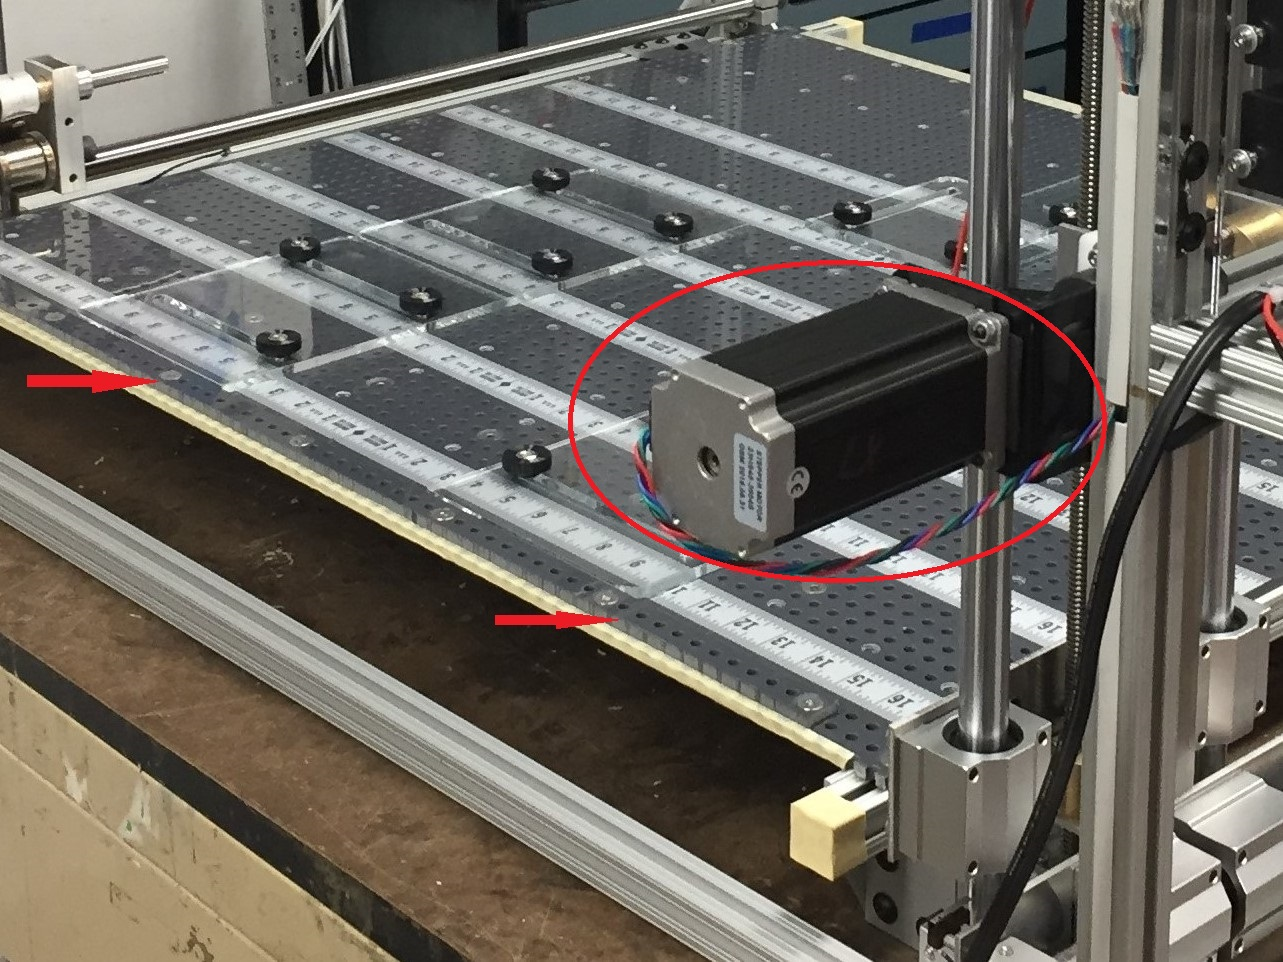
\includegraphics[width = 0.8\linewidth]{./Figures/panel.jpg}
	\caption{Work Panel Guiding Block Orientation }
	\label{fig:panel2}
\end{figure}
To install the work panel, first slide the work panel into the 4 supporting rods at the 4 corners with the correct orientation. Make sure all 4 corners sit securely in the supporting rods, then tighten all 8 thumb screws.

\newpage
\subsection{Install the Wire}
The wire is held to tension of approximately 10 lbs with a constant force spring. To install the wire, follow the steps shown below.

\begin{enumerate}[itemsep = 5pt,topsep=0pt]
\begin{figure}[H]
	\centering
	\begin{subfigure}[b]{.475\textwidth}
		\centering
		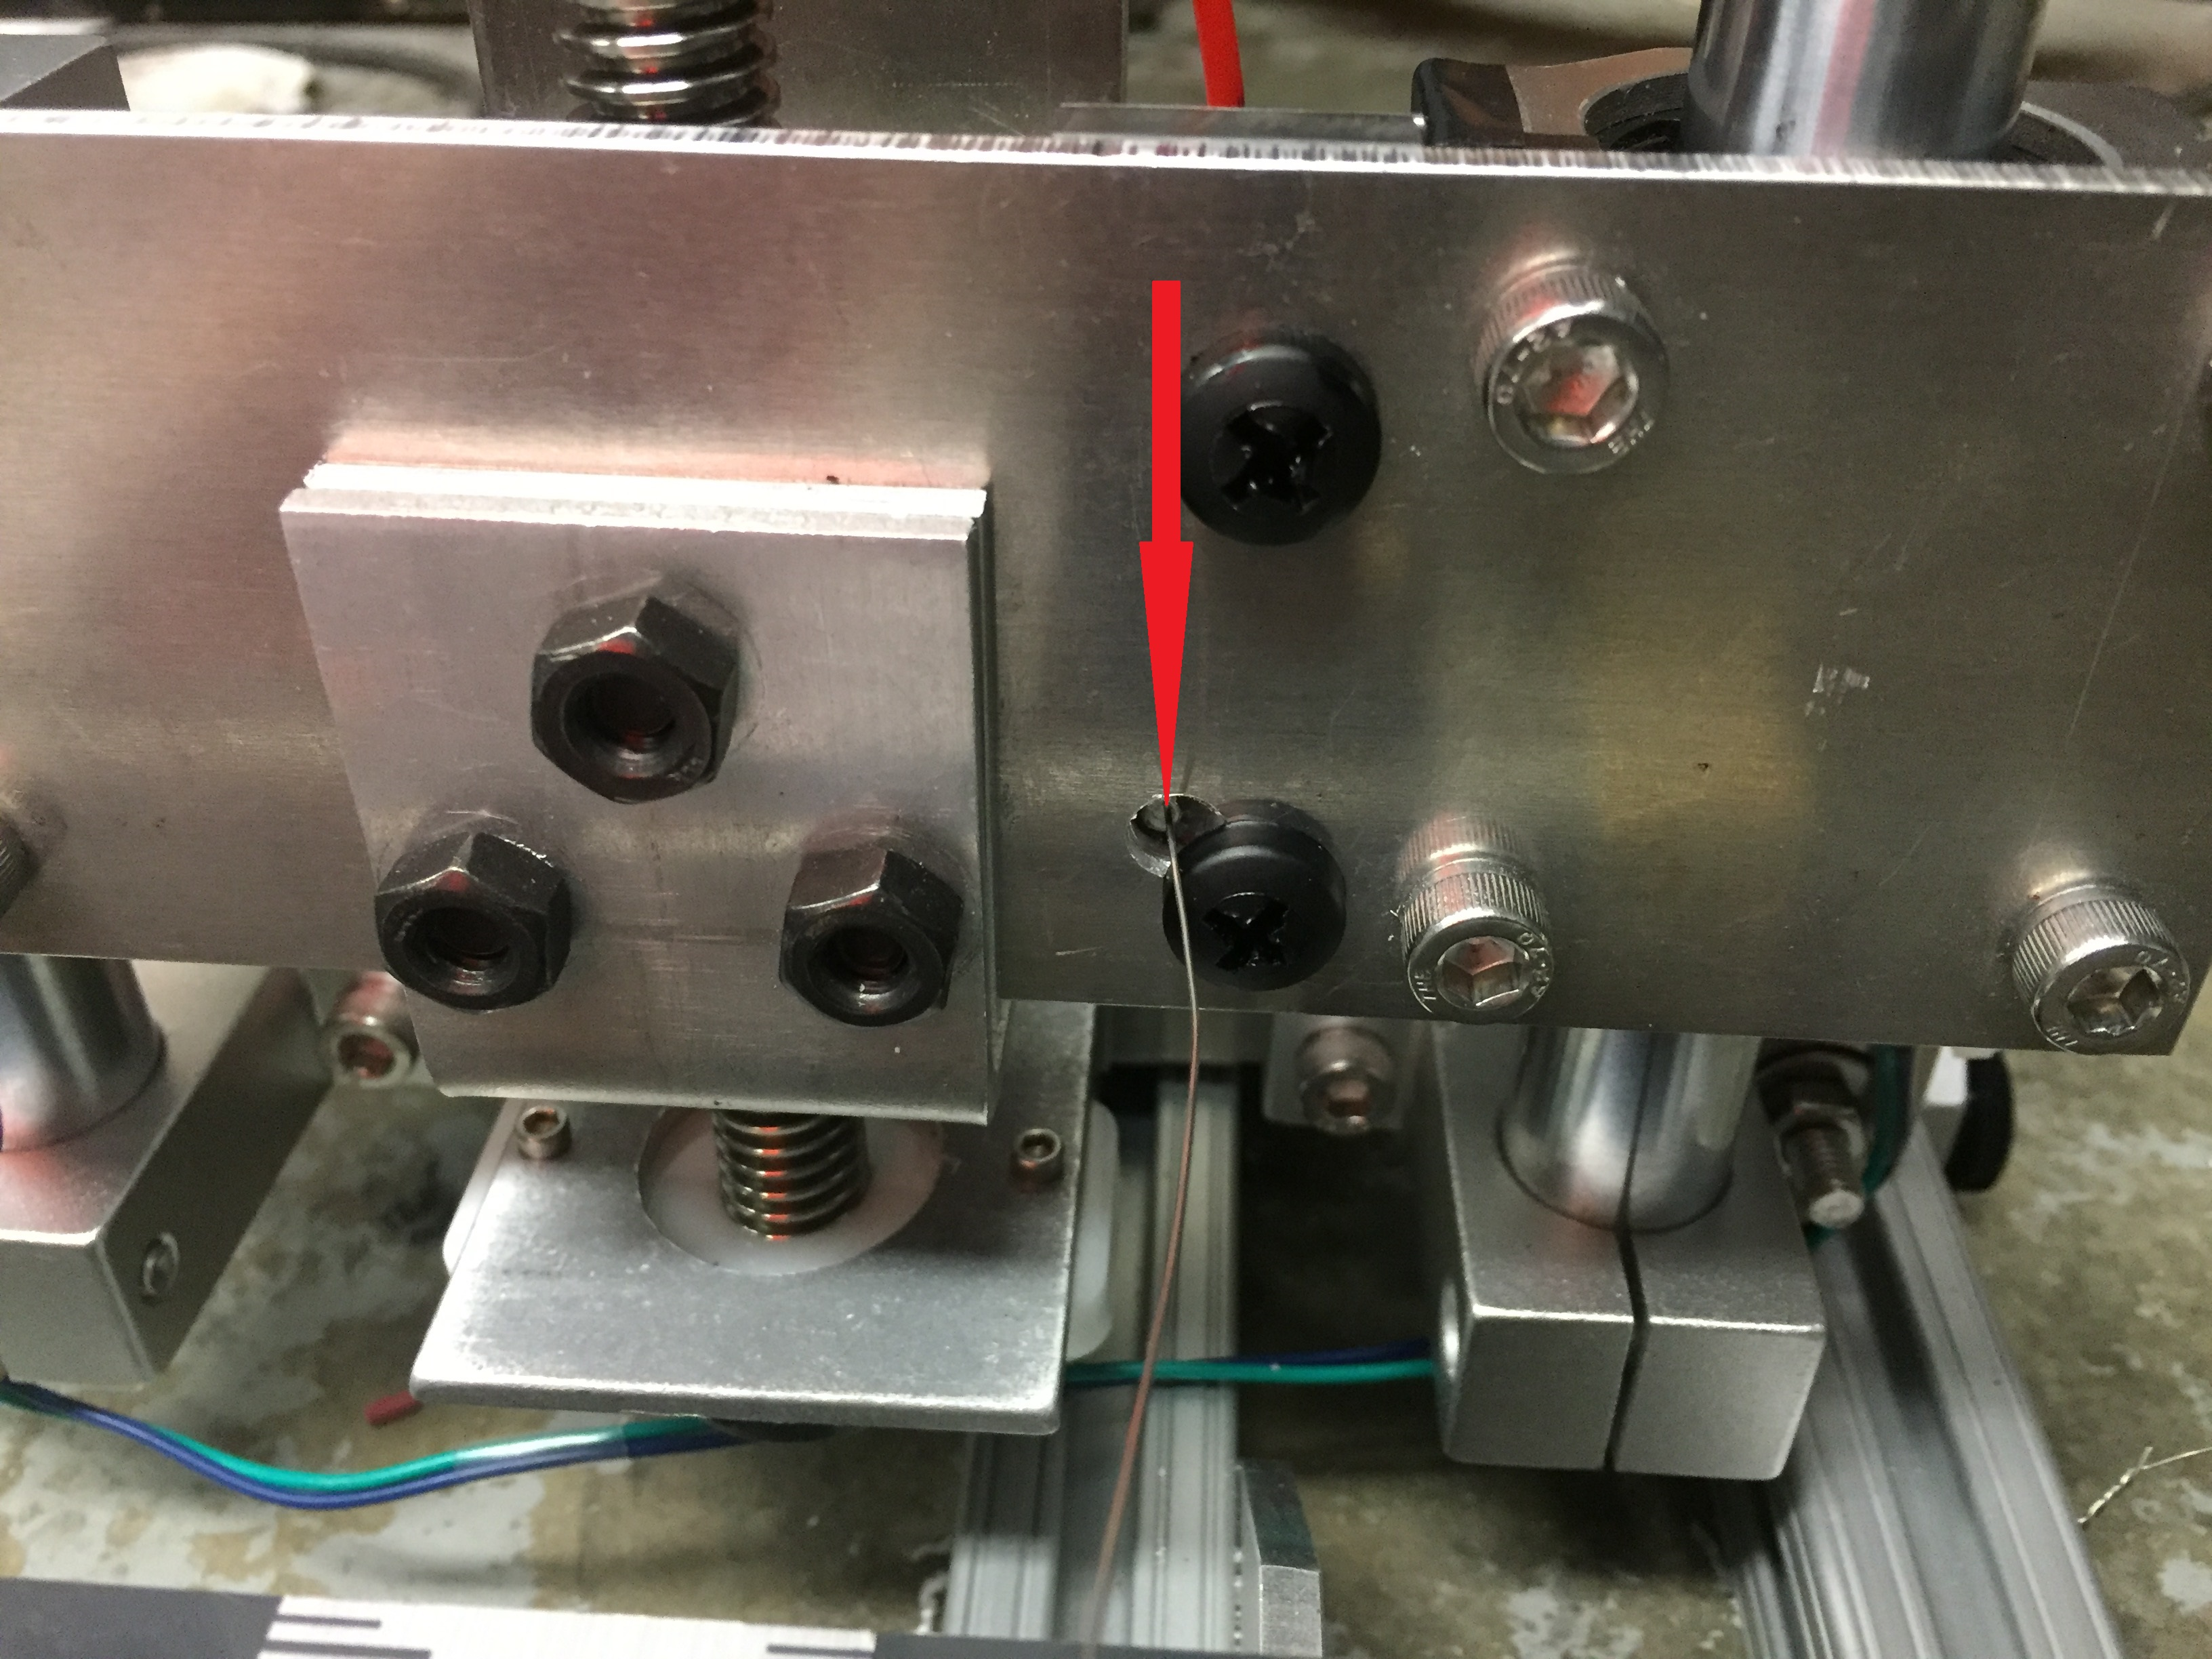
\includegraphics[width=\textwidth]{./Figures/Wire_mounting/1.jpg}
		\caption{Step 1}
	\end{subfigure}
	\begin{subfigure}[b]{.475\textwidth}
		\centering
		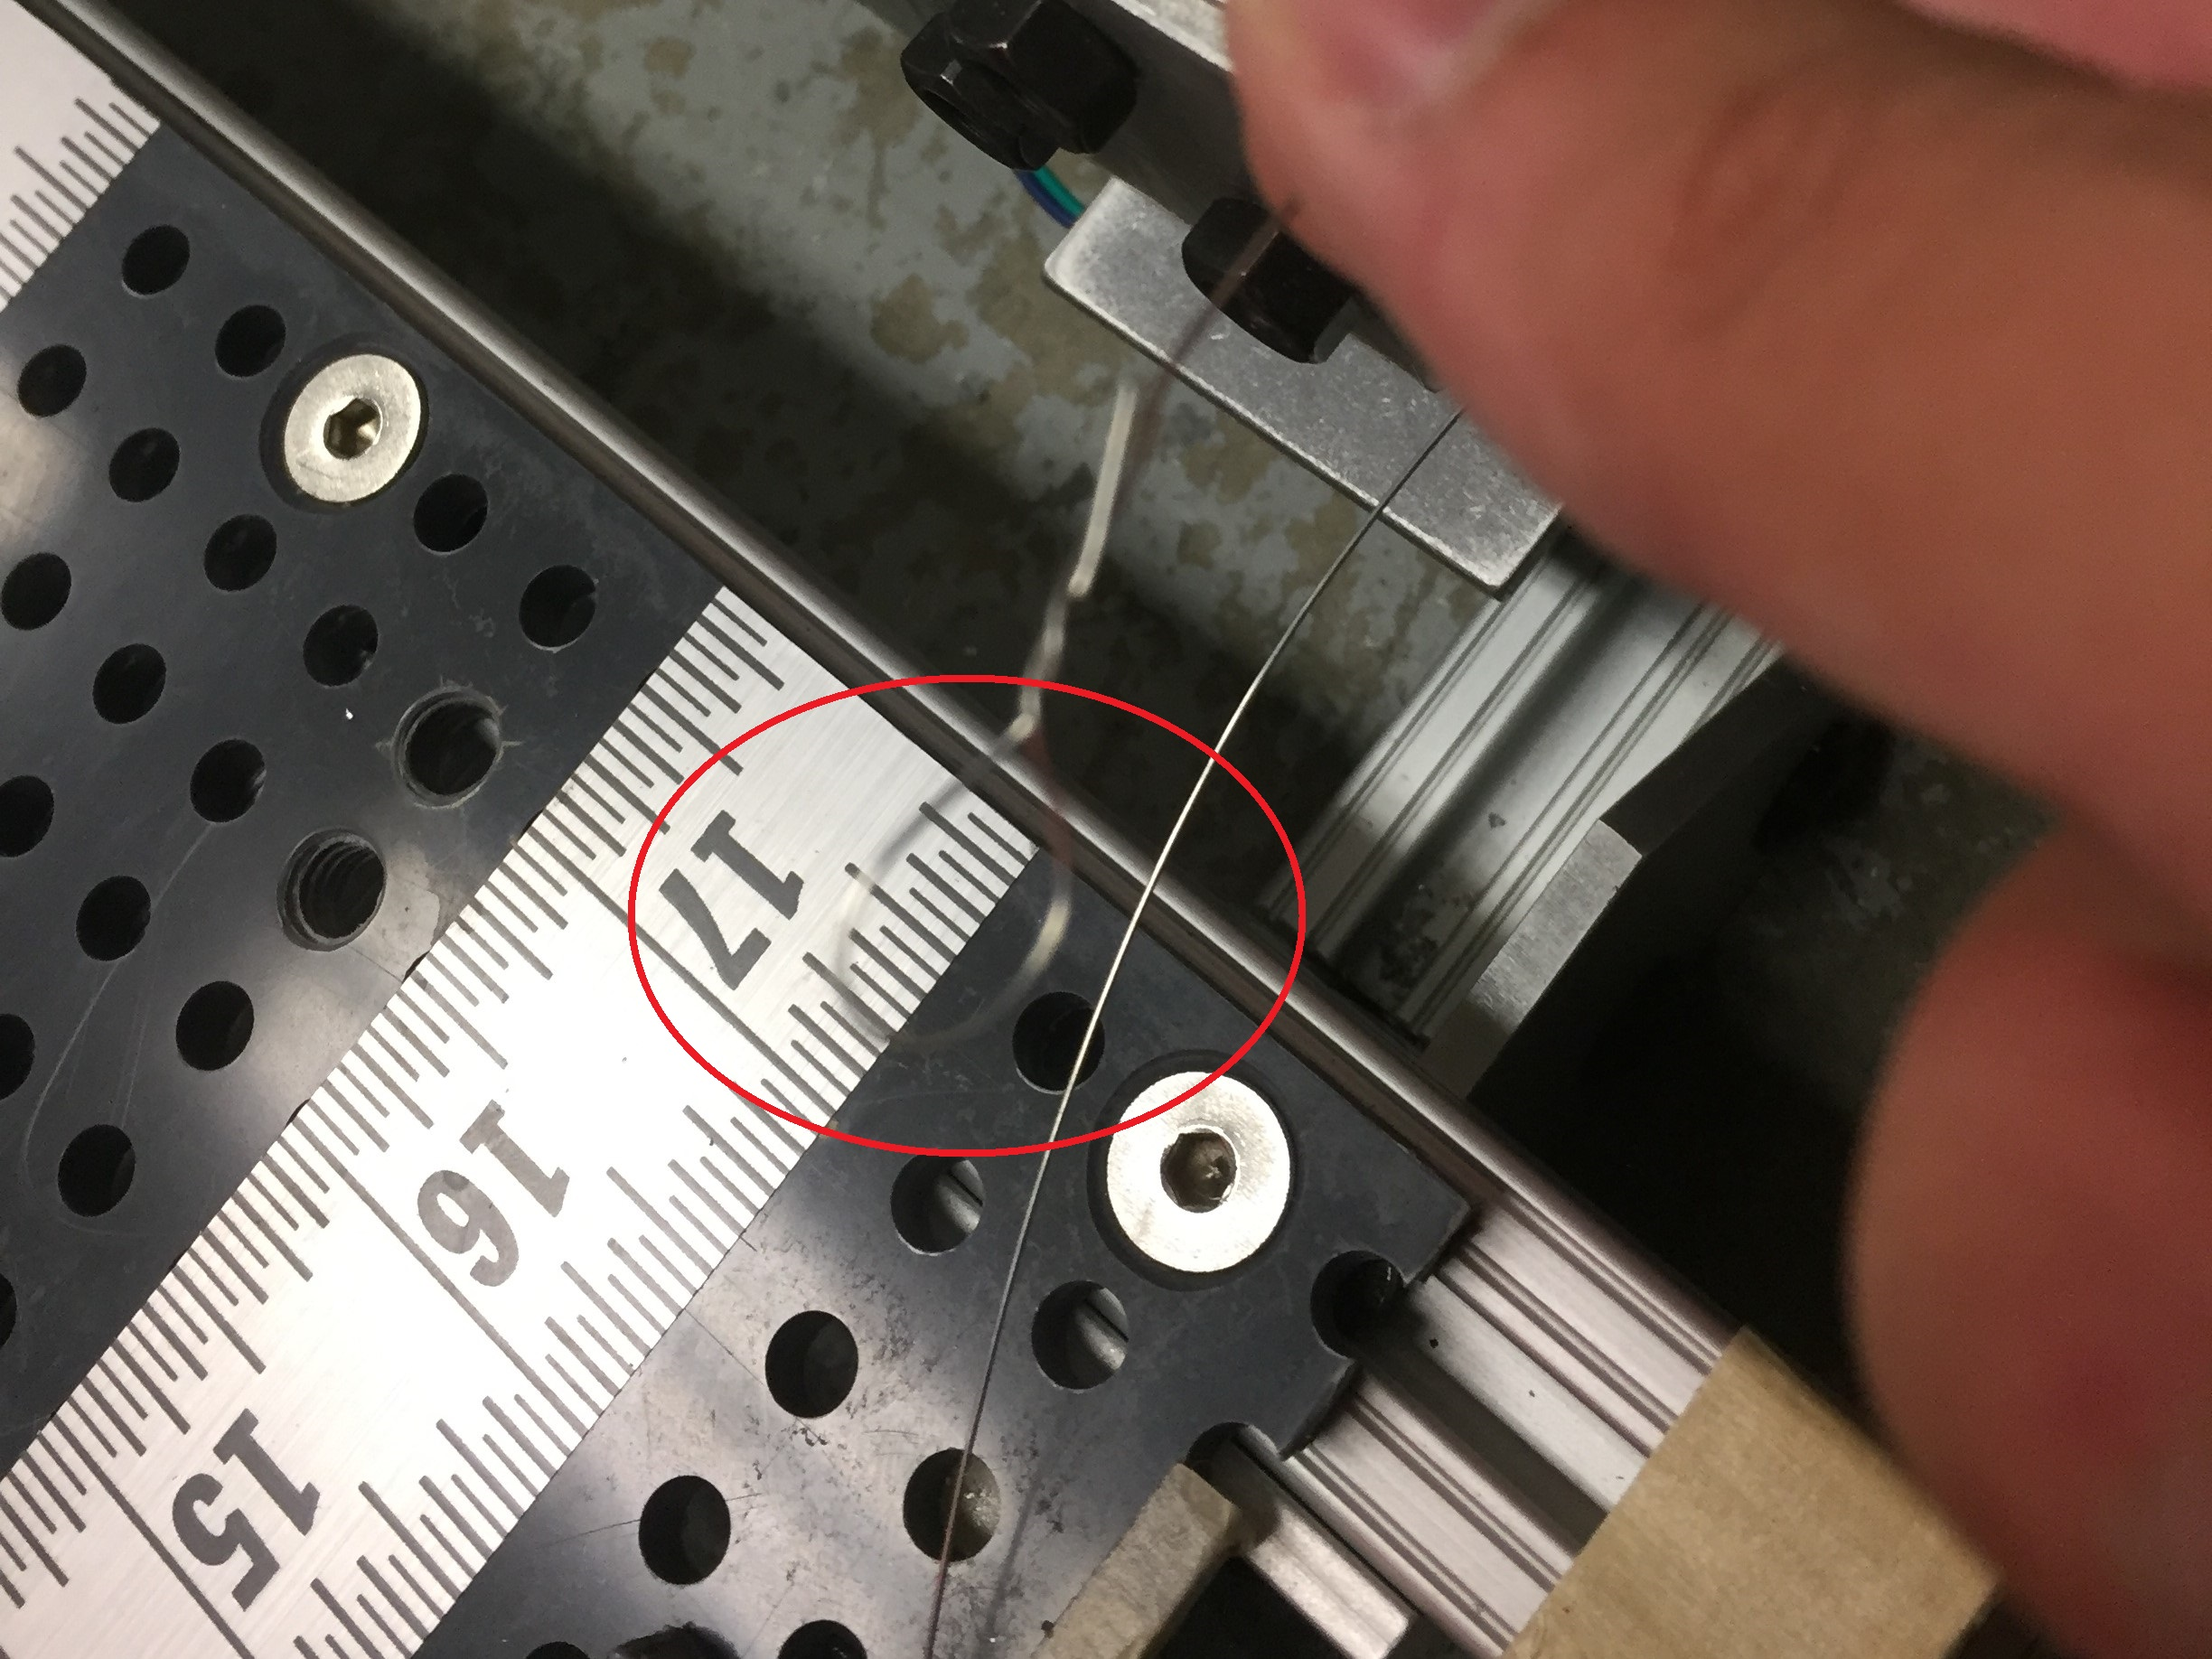
\includegraphics[width=\textwidth]{./Figures/Wire_mounting/2.jpg}
		\caption{Step 2}
	\end{subfigure}
	\centering
	\begin{subfigure}[b]{.475\textwidth}
		\centering
		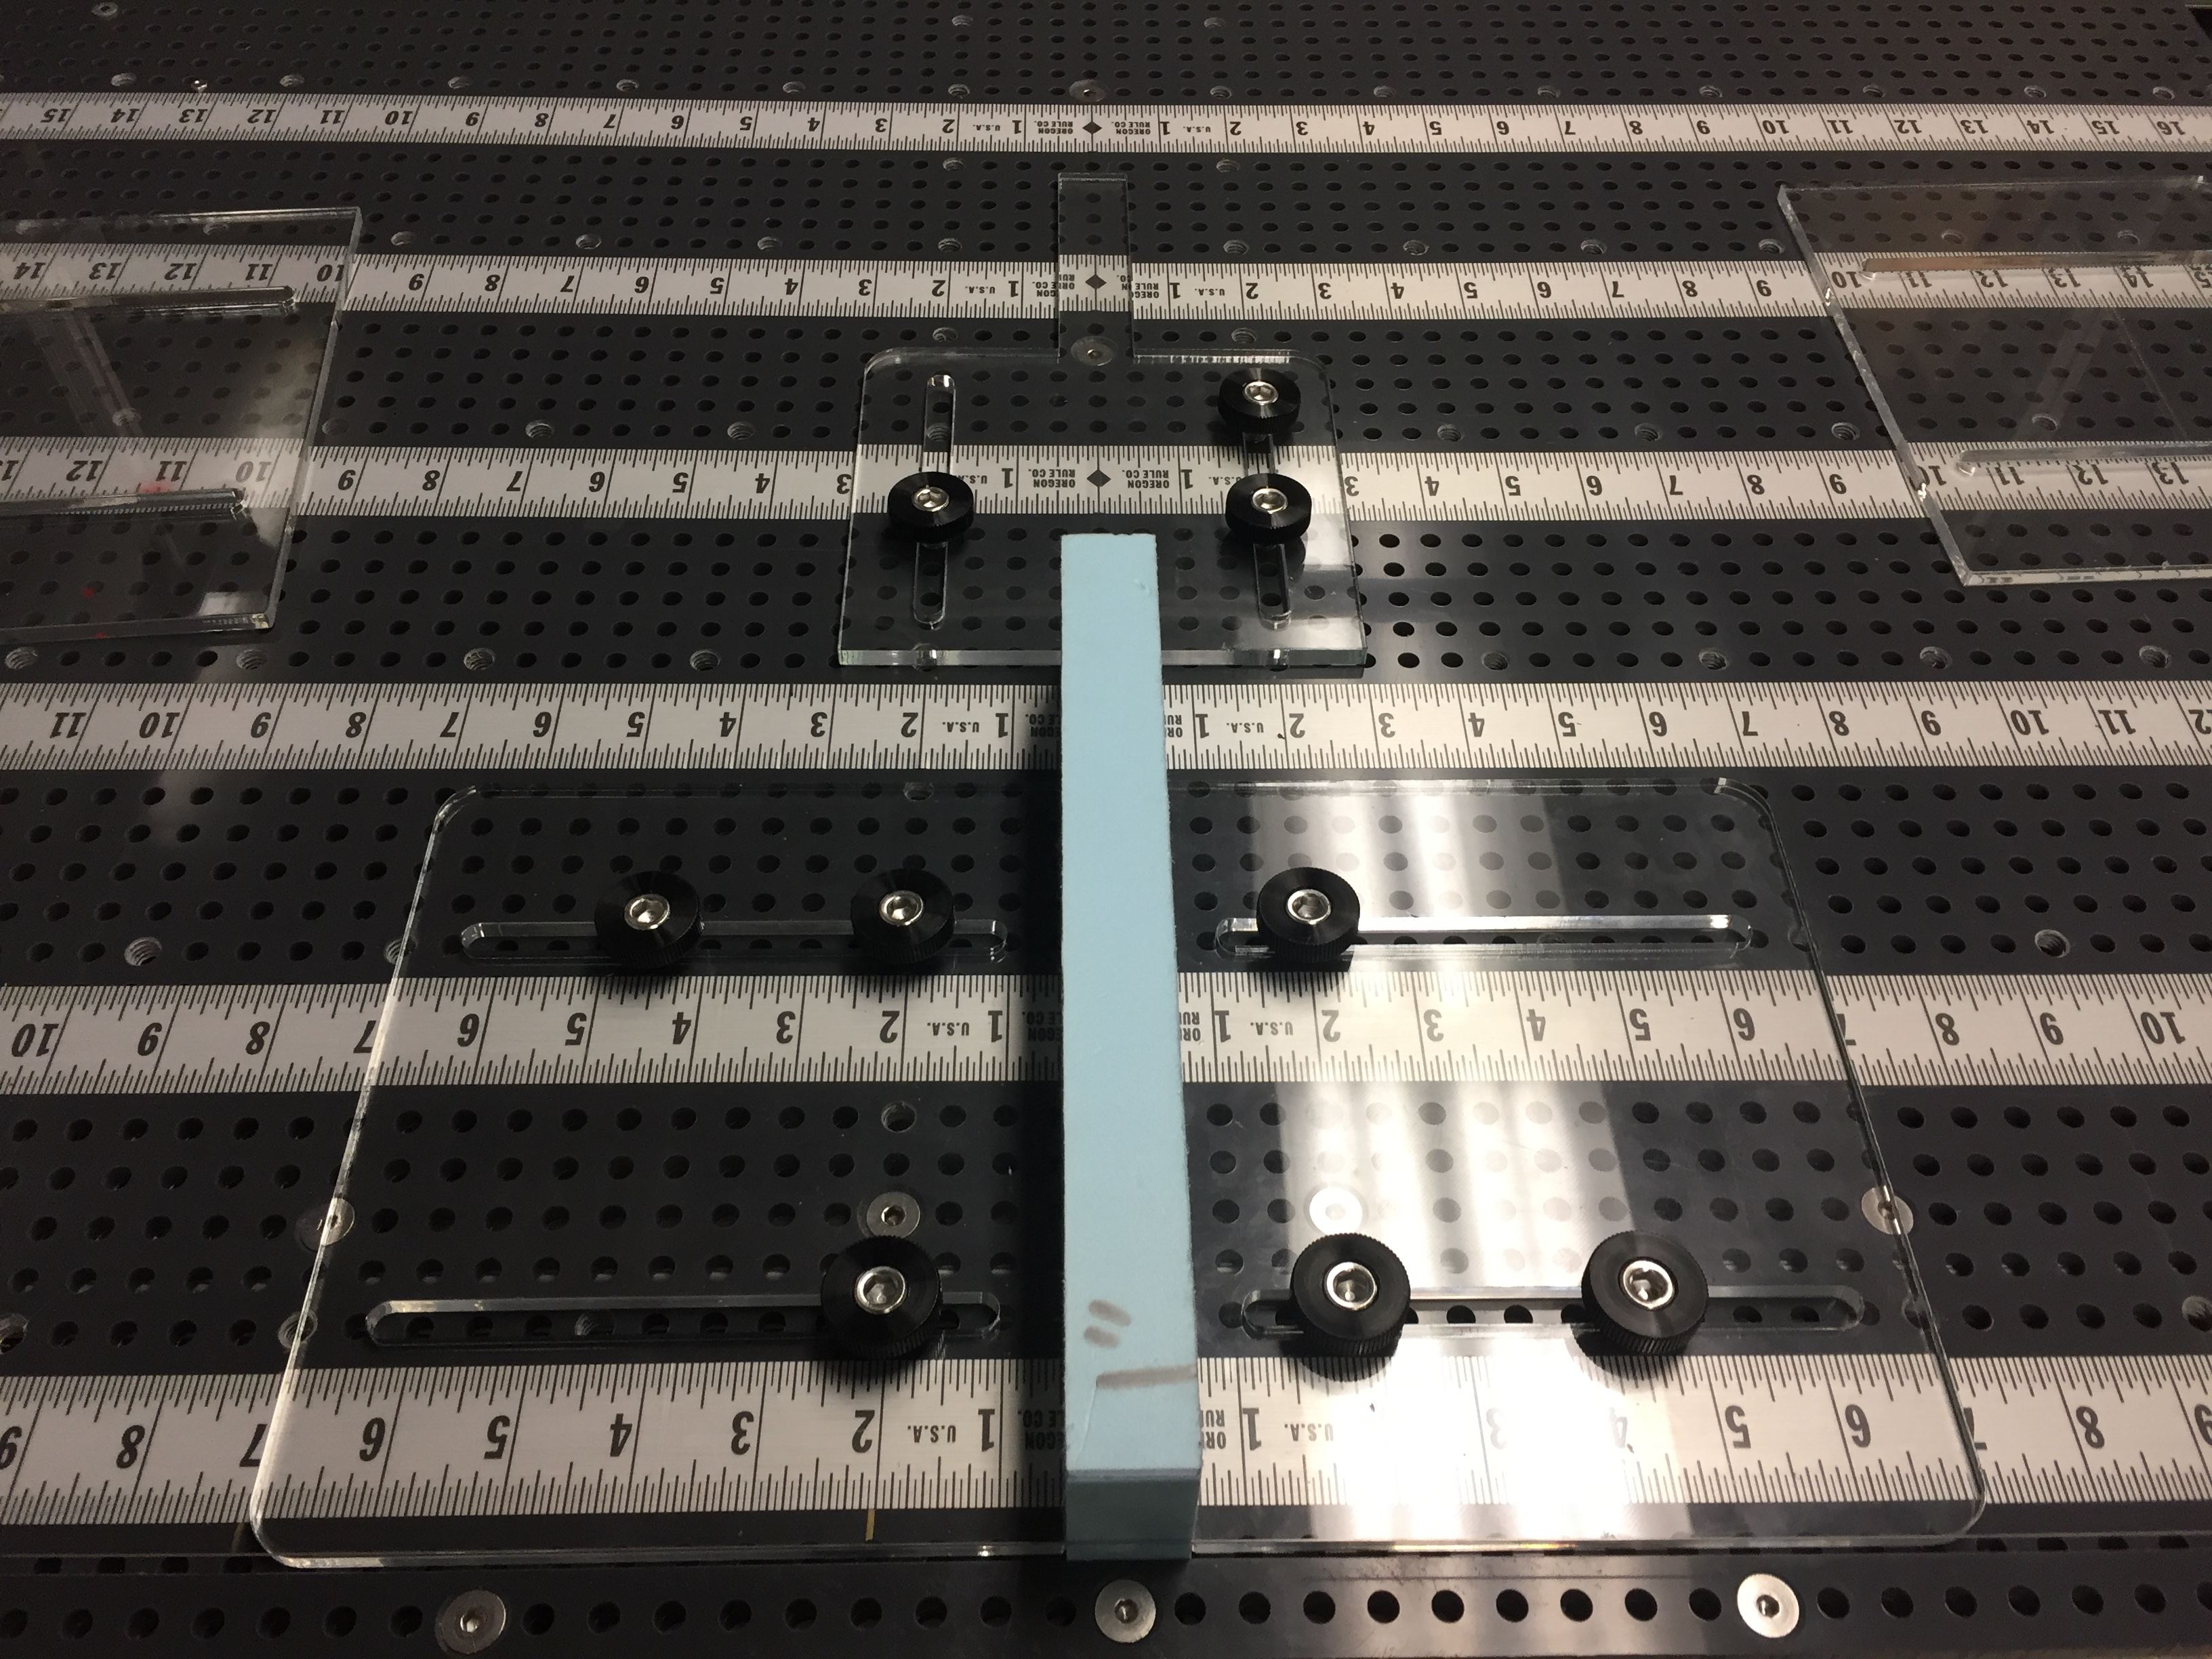
\includegraphics[width=\textwidth]{./Figures/Wire_mounting/3.jpg}
		\caption{Step 3}
	\end{subfigure}
	\begin{subfigure}[b]{.475\textwidth}
		\centering
		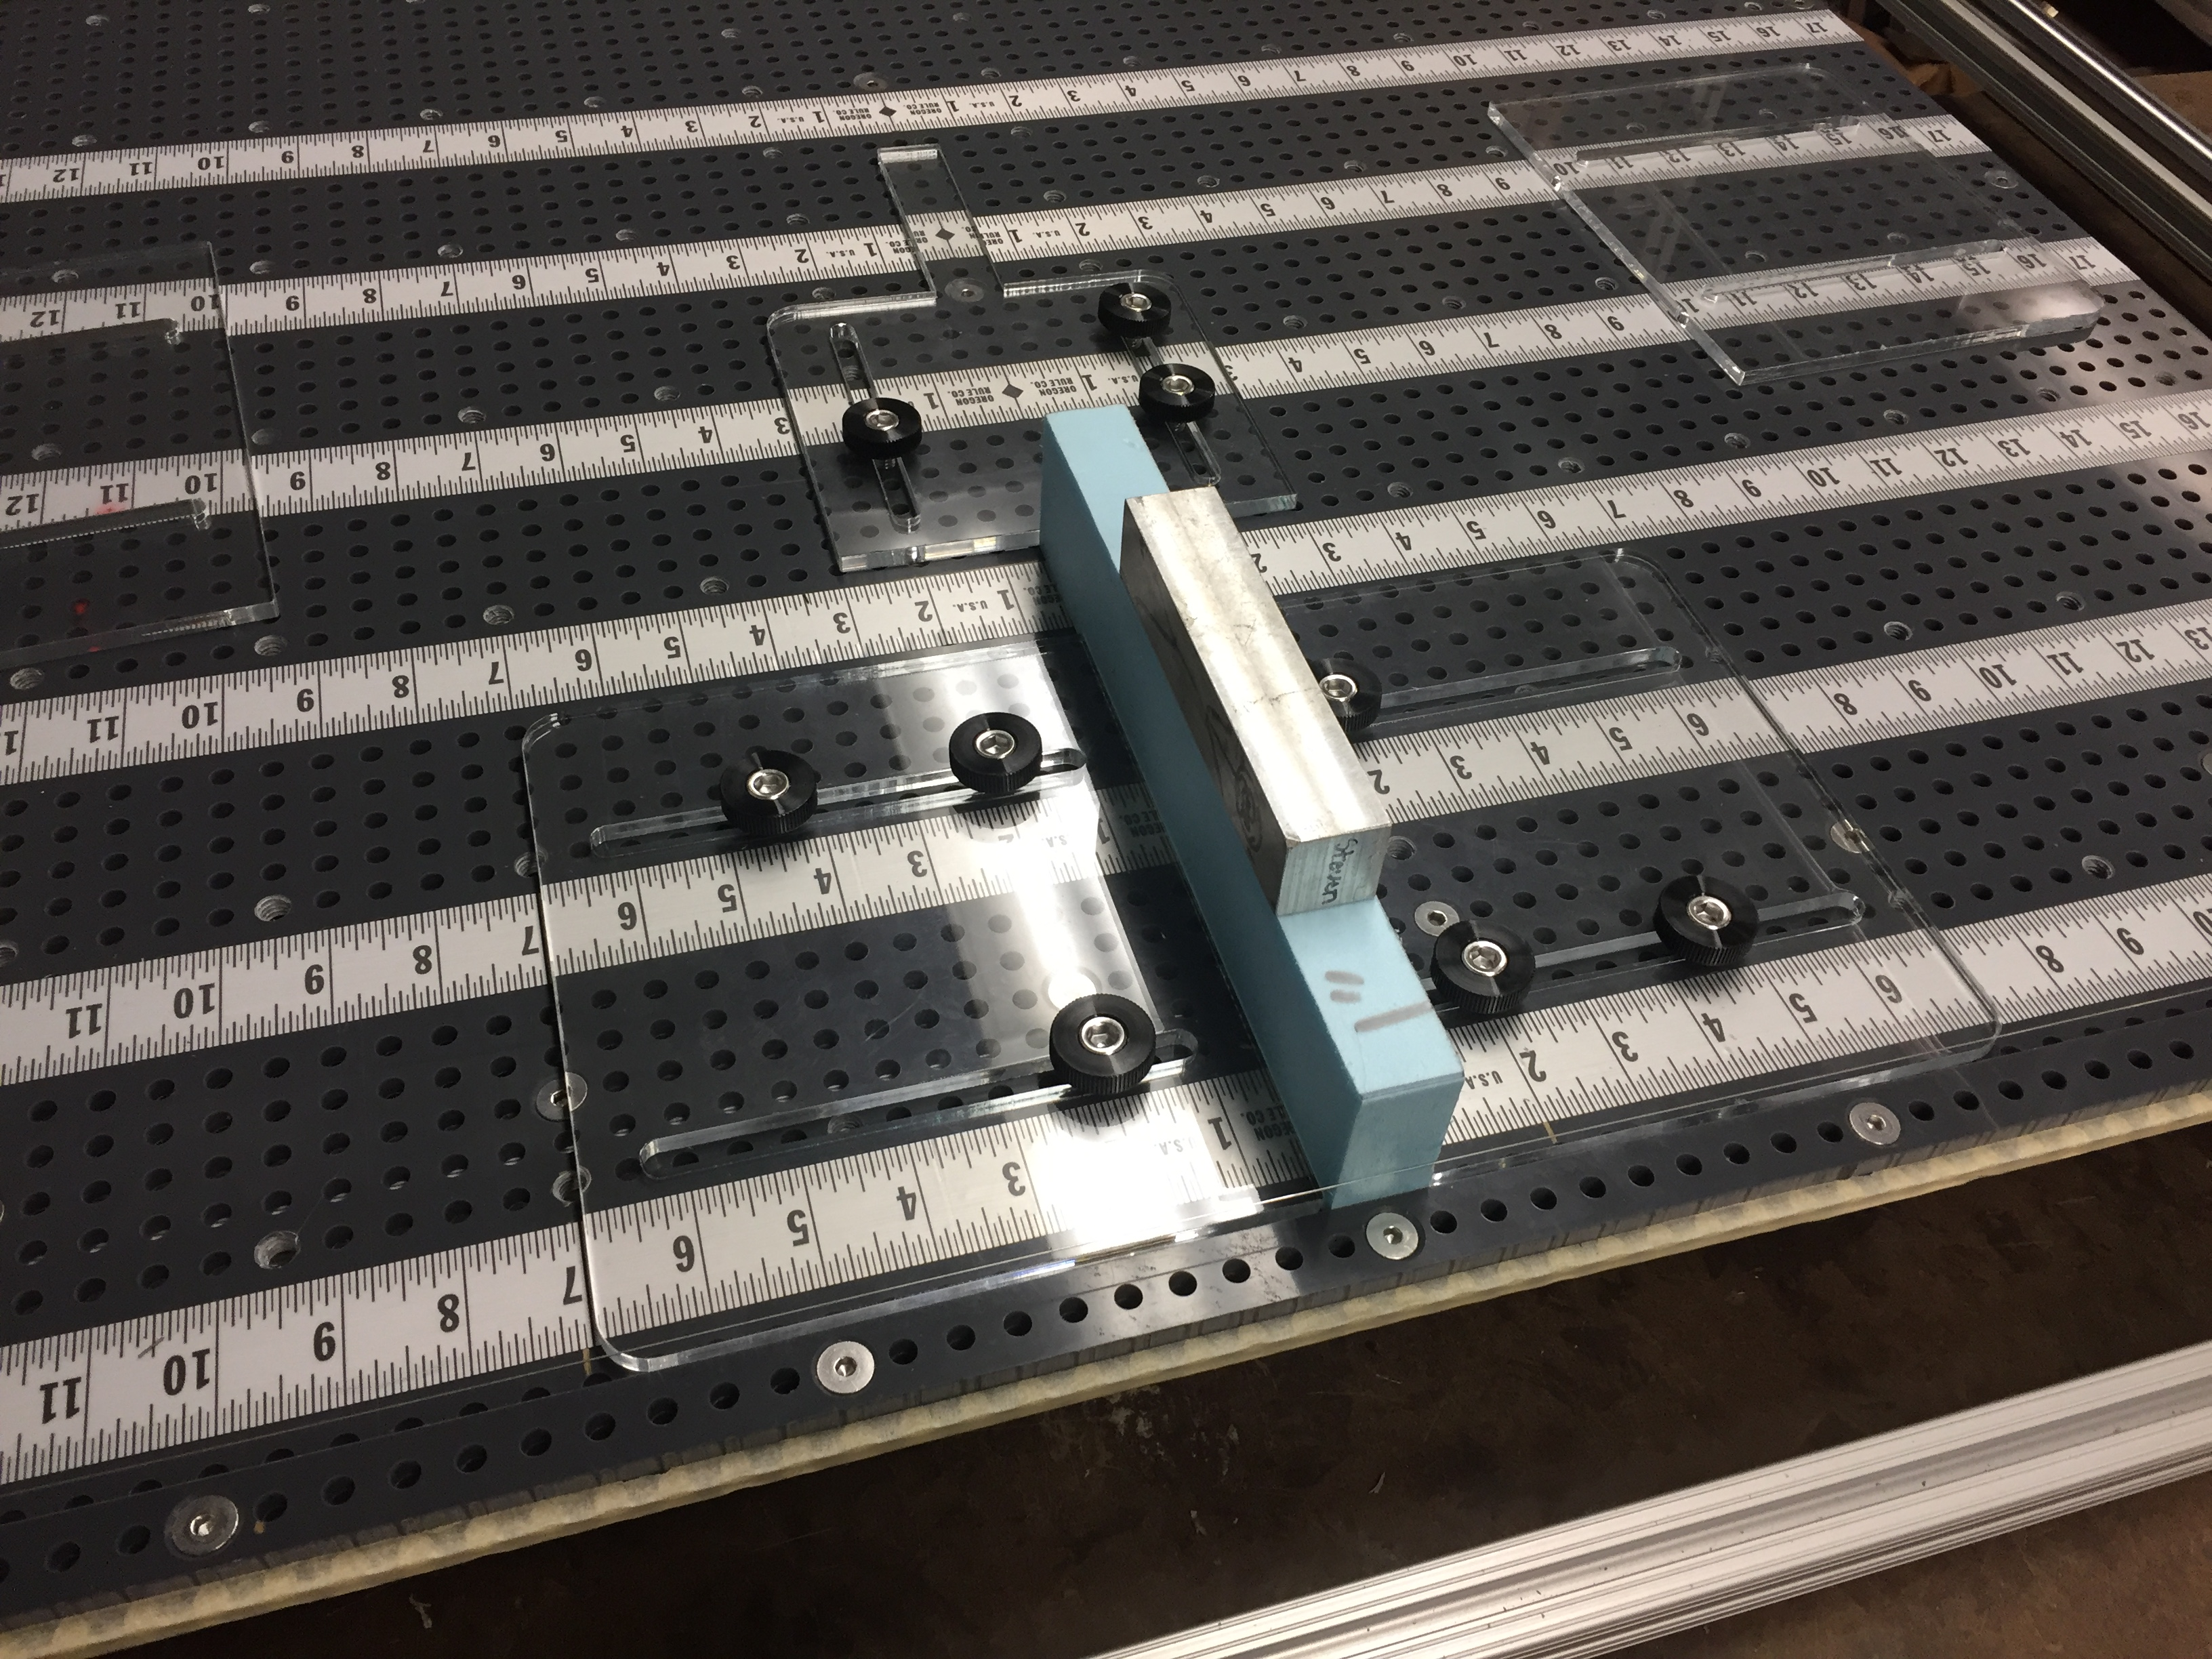
\includegraphics[width=\textwidth]{./Figures/Wire_mounting/4.jpg}
		\caption{Step 4}
	\end{subfigure}
	\caption{Steps 1-4}
\end{figure}

\item Feed the wire through the small guiding hole on the side without the pulley.
\item Make a hoop at the end of the wire.
\item Put the hoop around the Nylon bolt and straighten the wire across the entire span of the foamcutter.
\item Cut the wire at about 3ft longer than the span of the foamcutter. Then feed the end of the wire through the small guiding hole on the side with the pulley.

\begin{figure}[H]
	\centering
	\begin{subfigure}[b]{.475\textwidth}
		\centering
		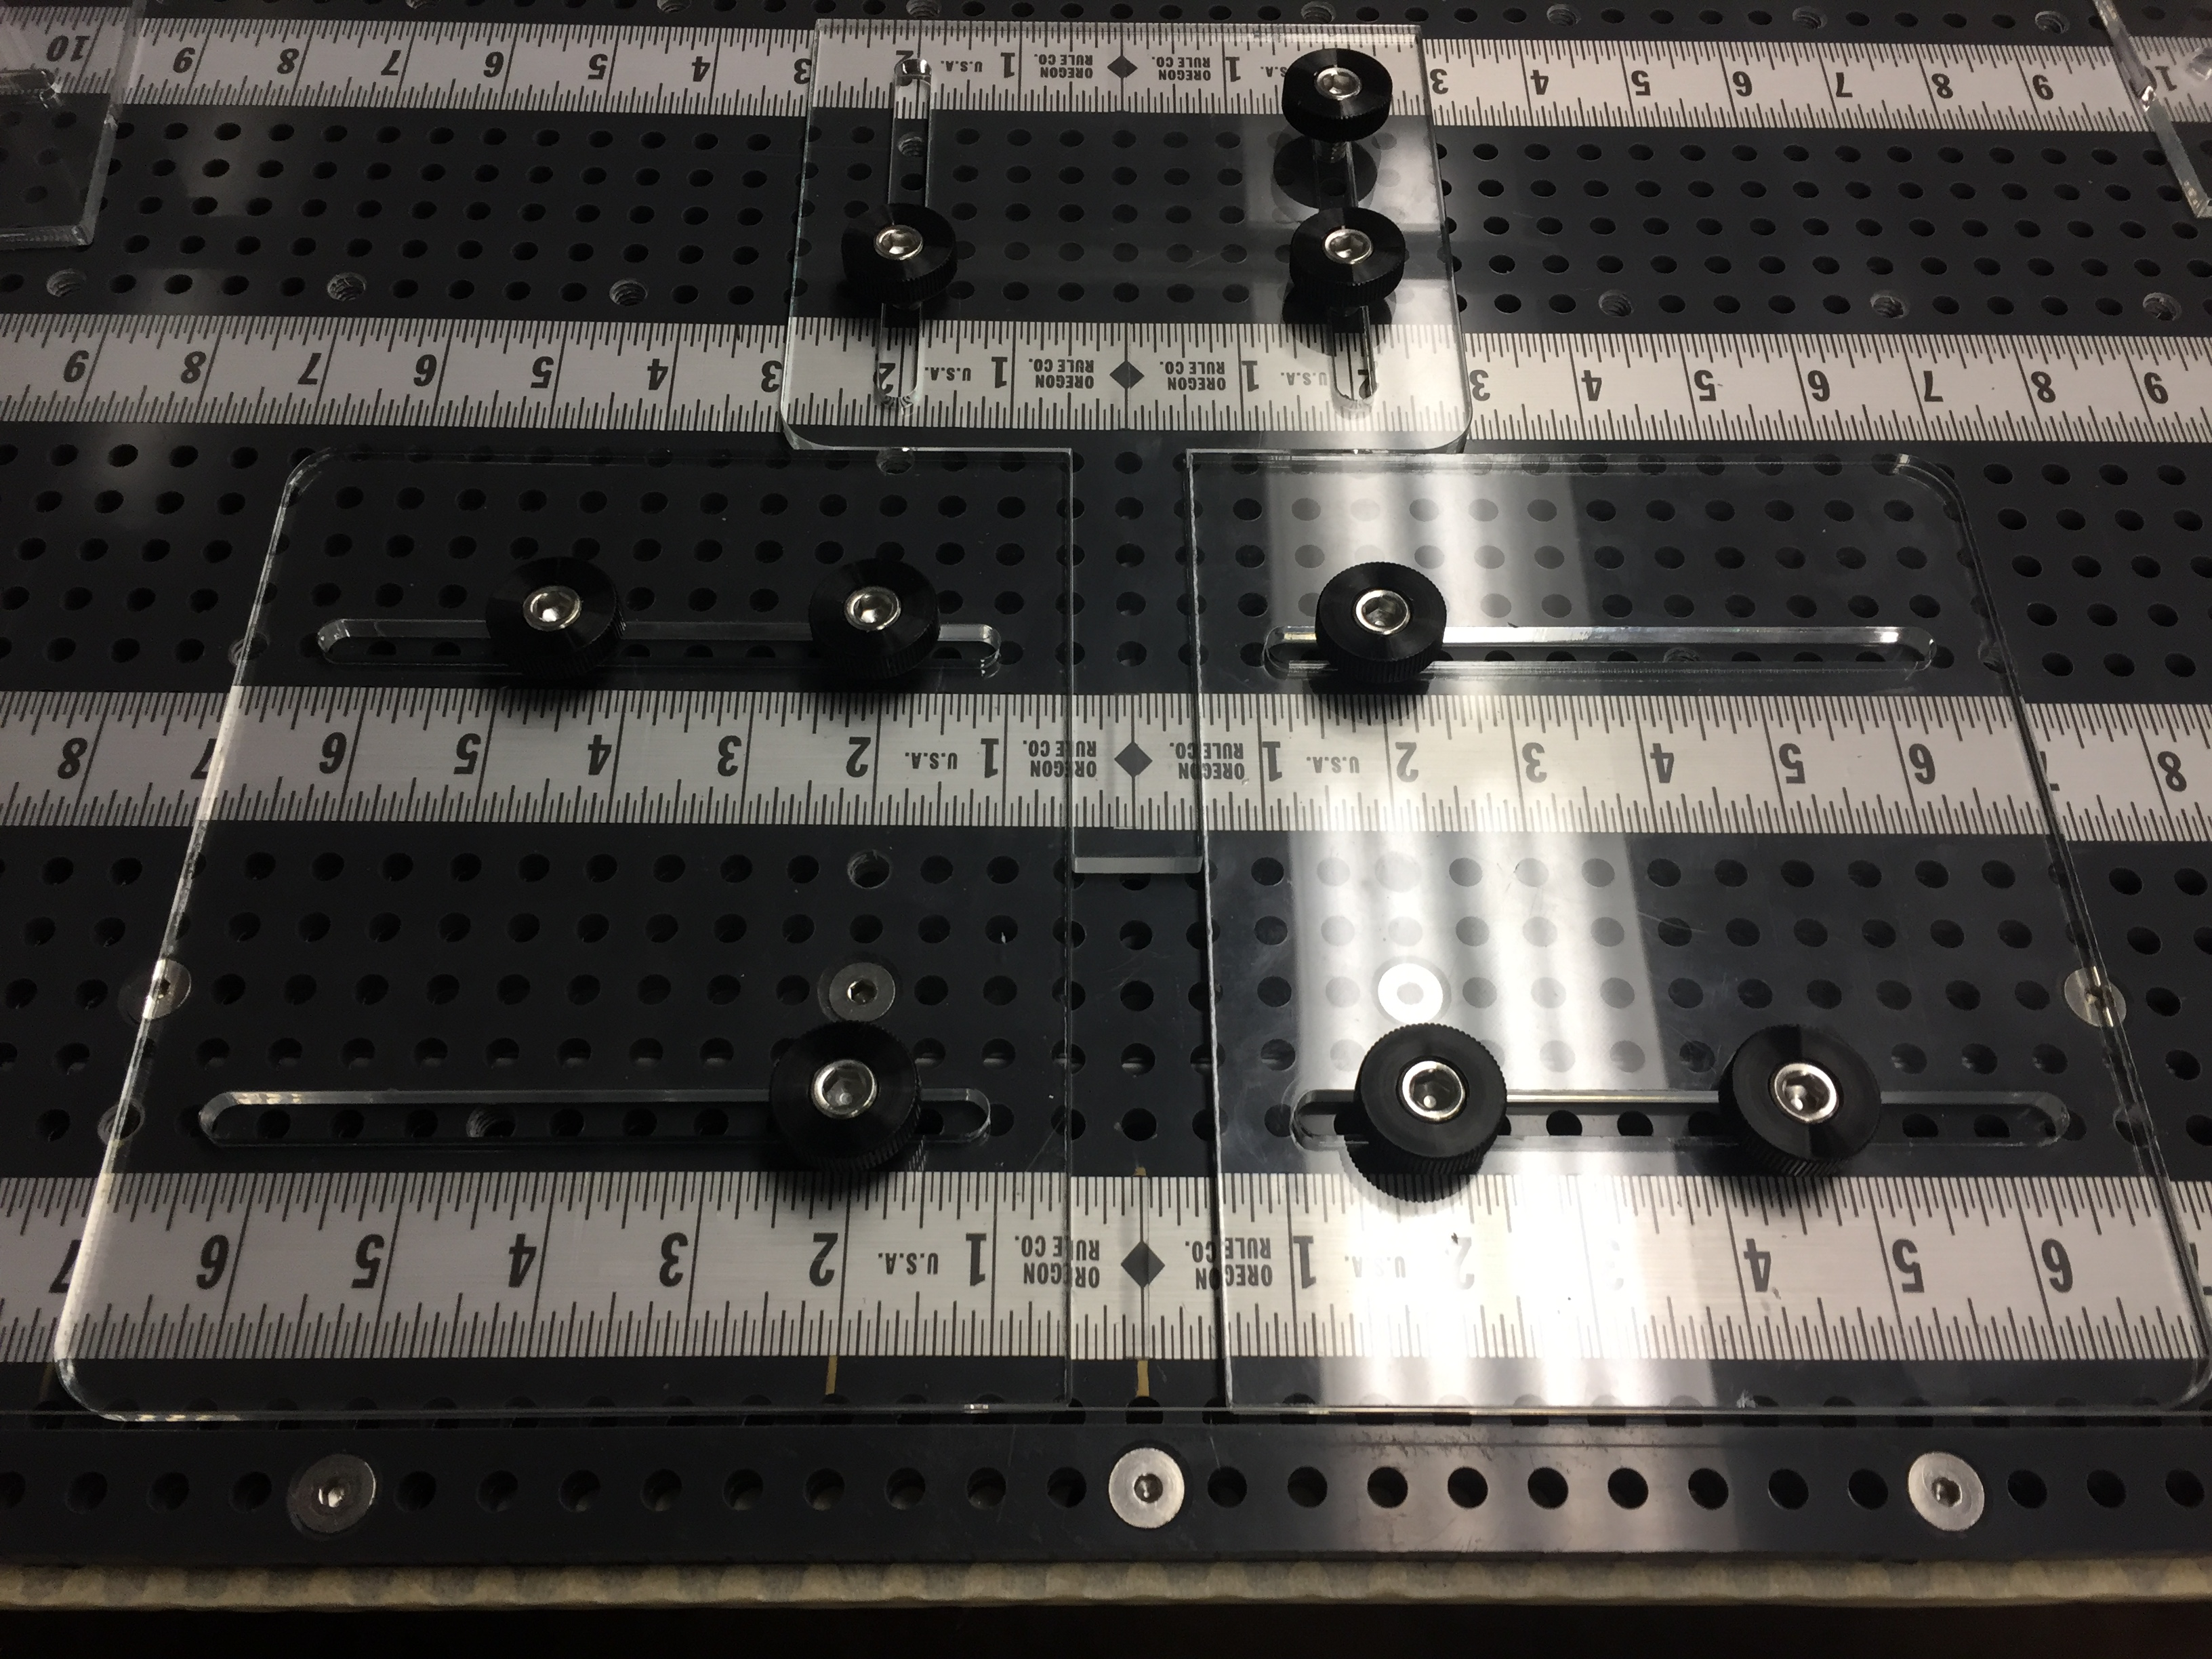
\includegraphics[width=\textwidth]{./Figures/Wire_mounting/5.jpg}
		\caption{Step 5}
	\end{subfigure}
	\begin{subfigure}[b]{.475\textwidth}
		\centering
		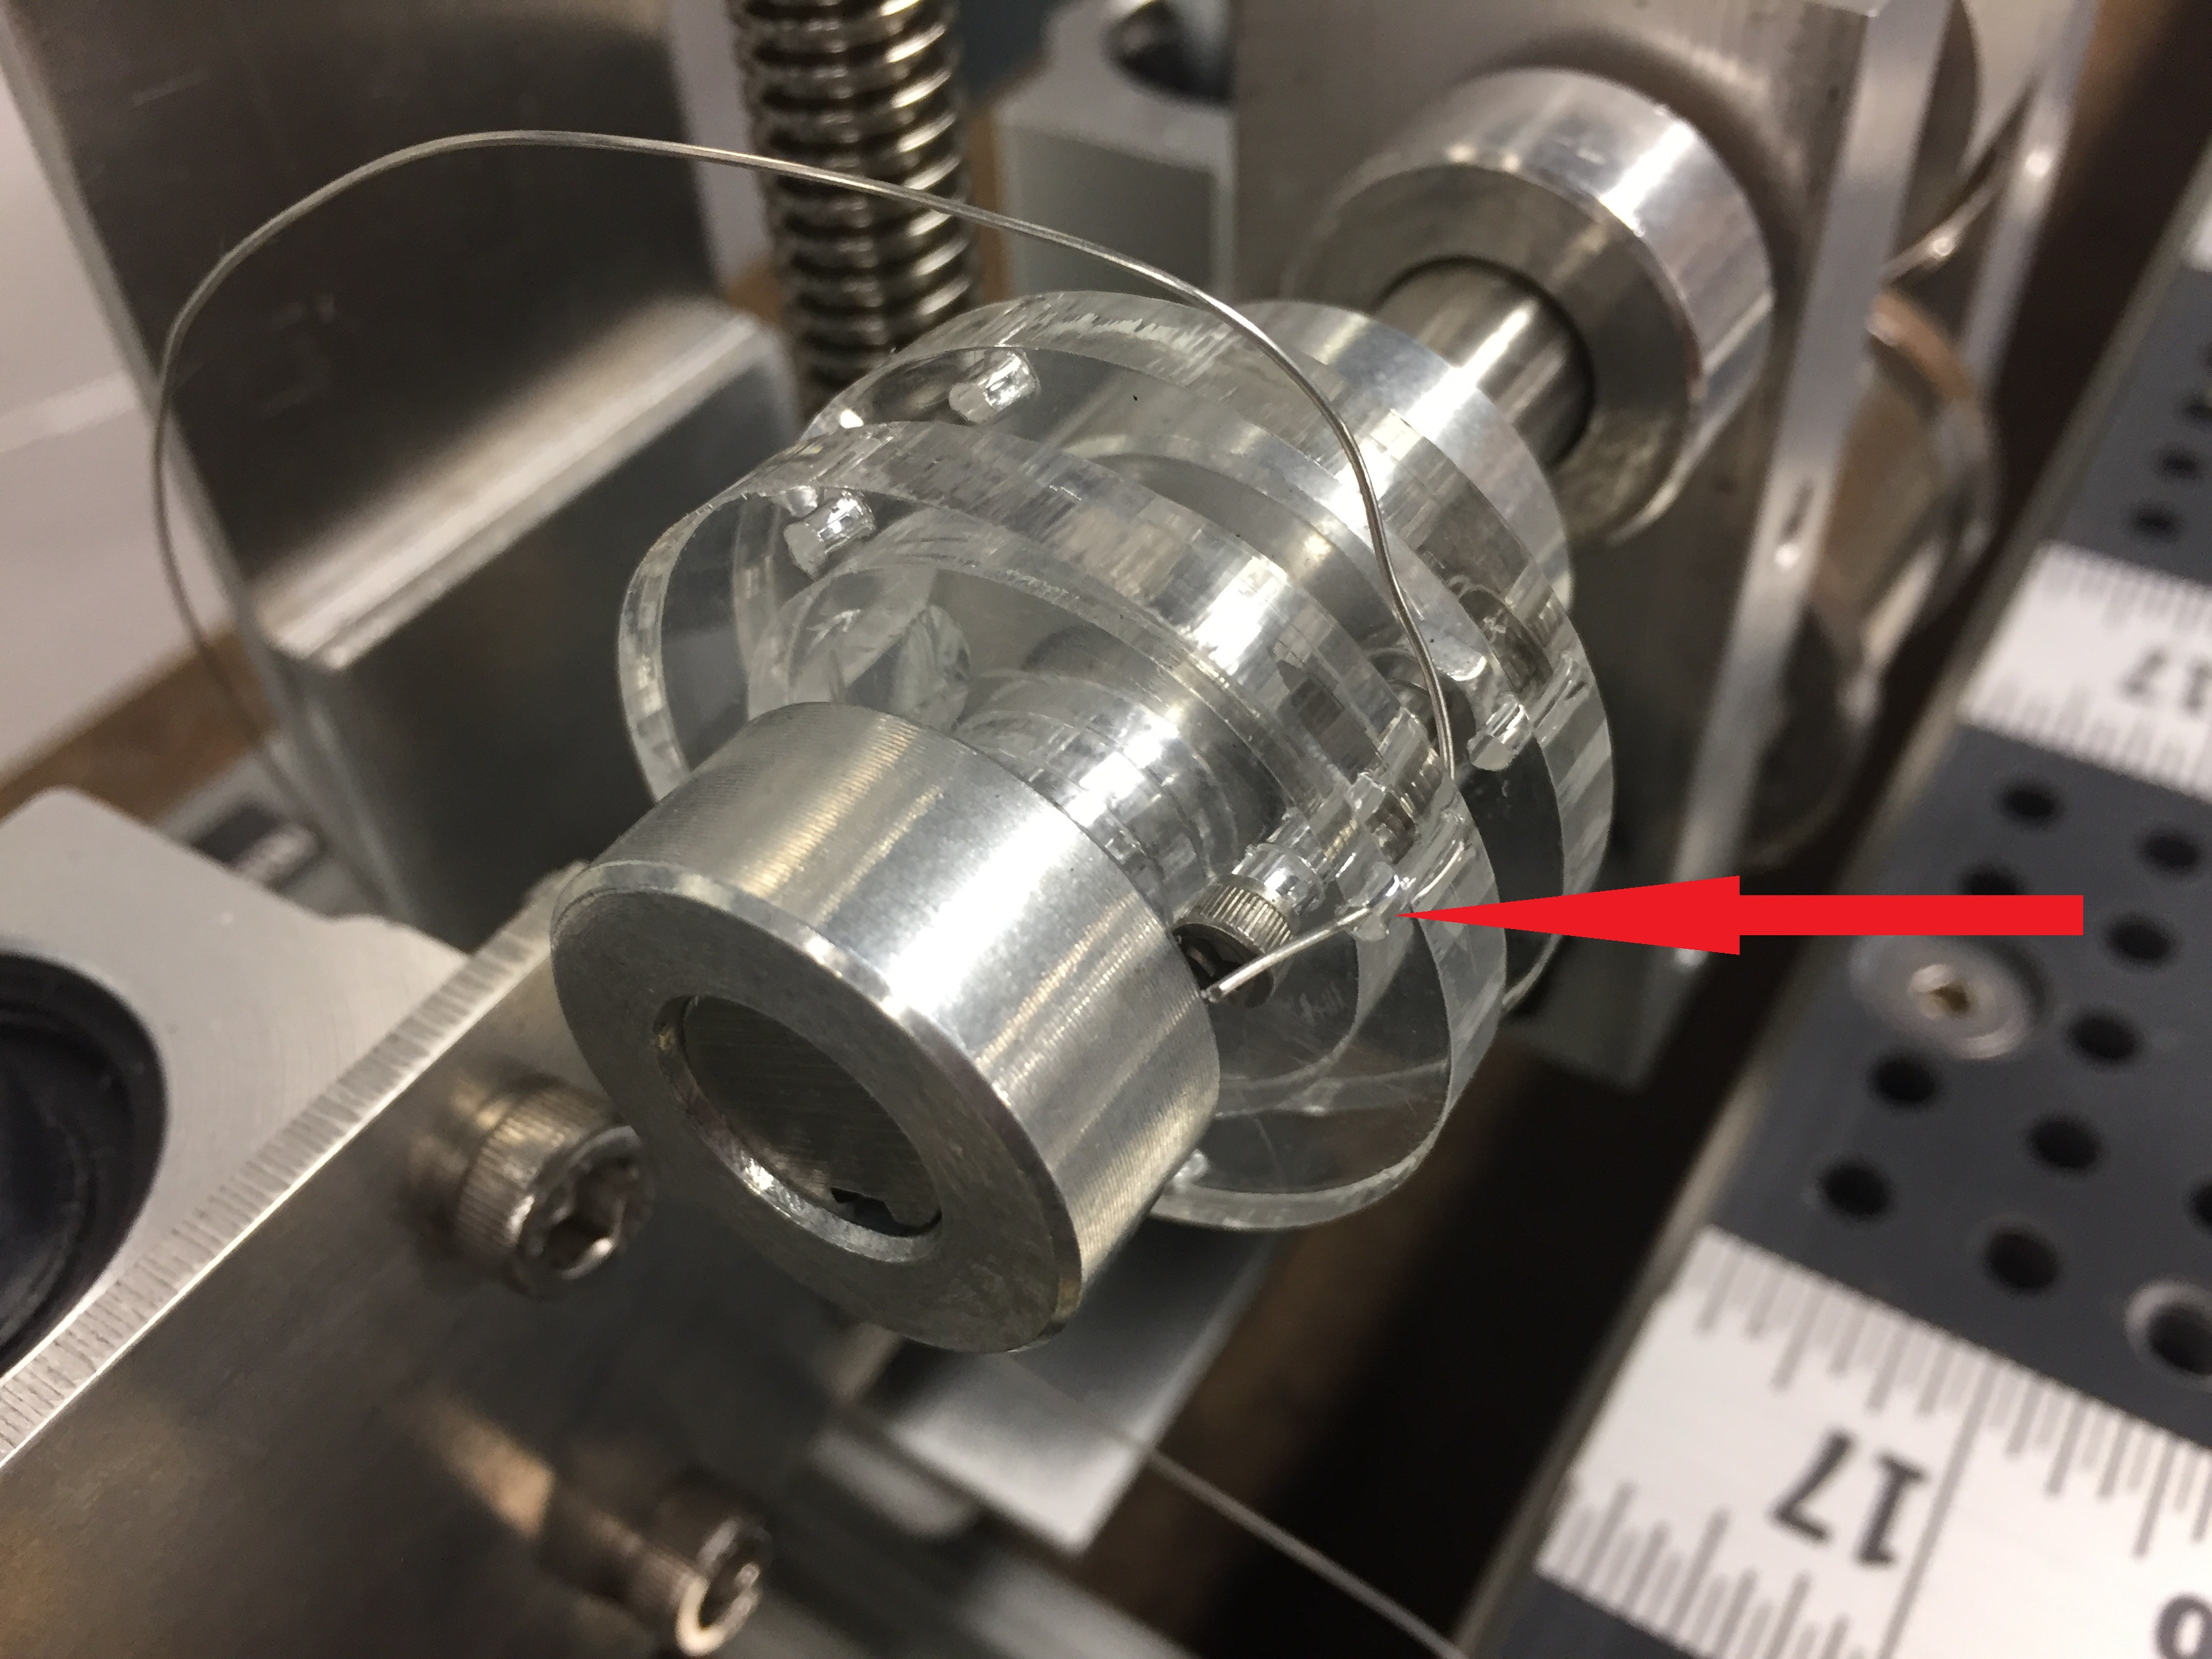
\includegraphics[width=\textwidth]{./Figures/Wire_mounting/6.jpg}
		\caption{Step 6}
	\end{subfigure}	
	\centering
	\begin{subfigure}[b]{.475\textwidth}
		\centering
		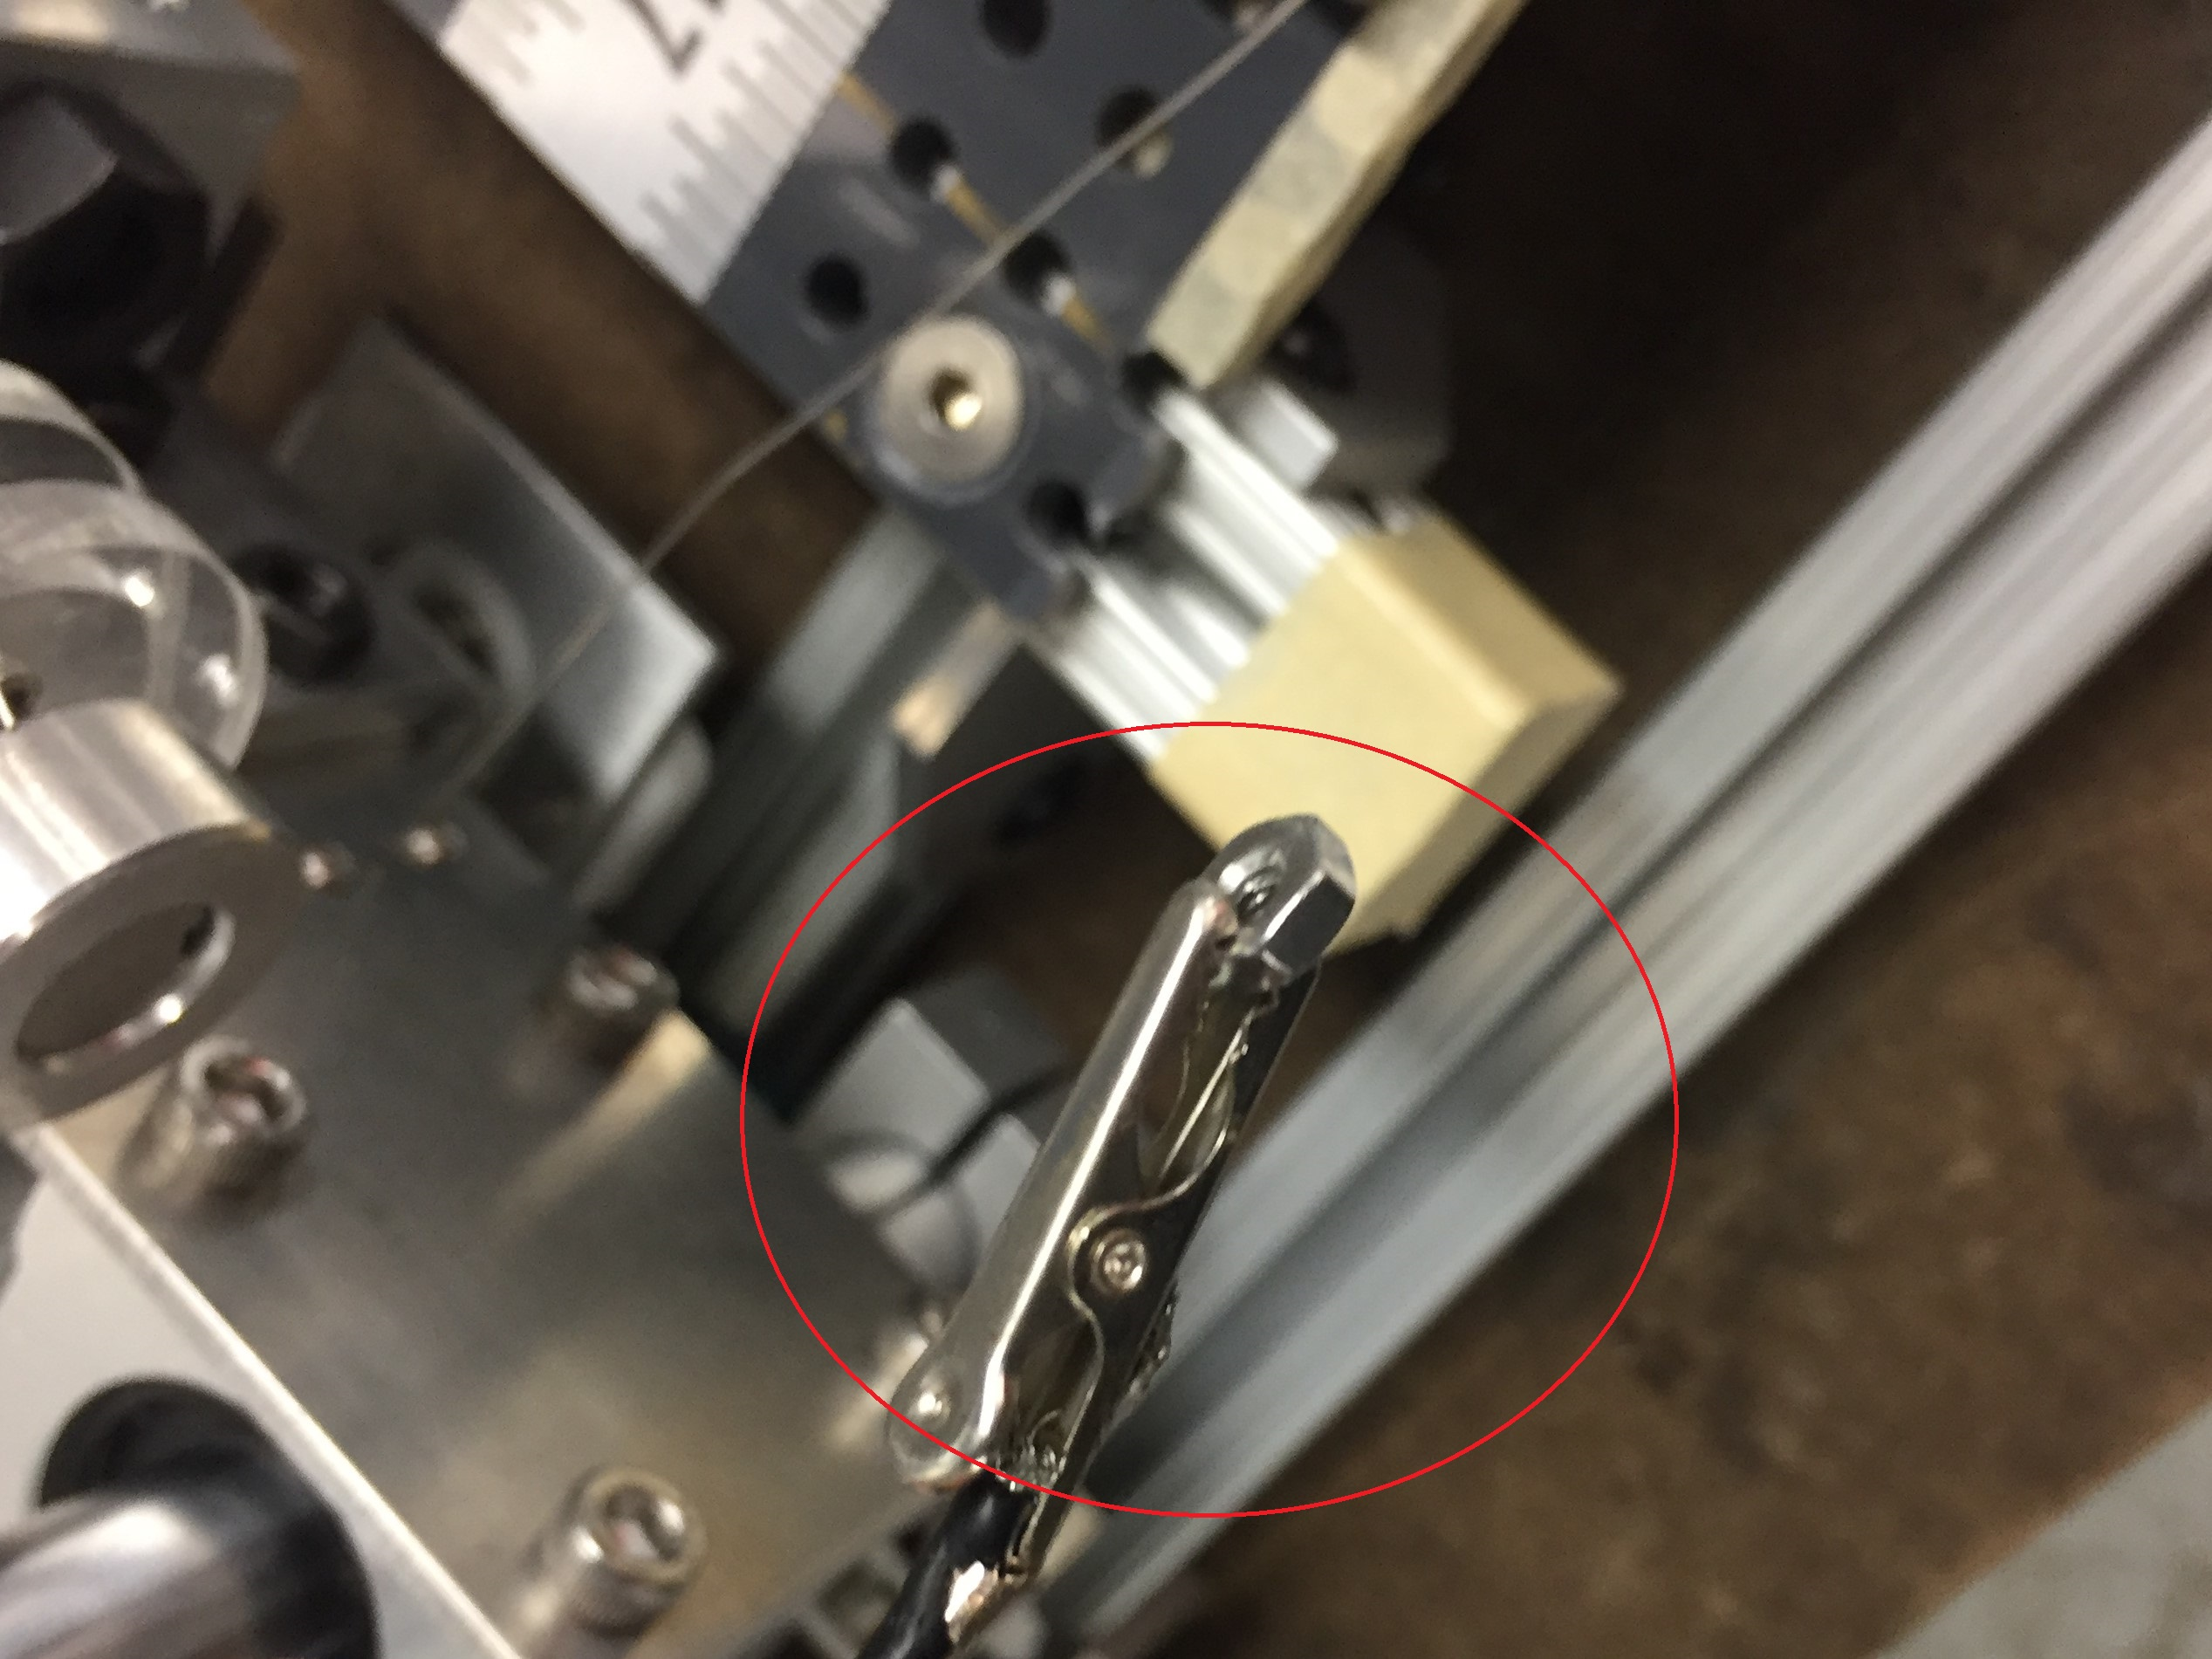
\includegraphics[width=\textwidth]{./Figures/Wire_mounting/7.jpg}
		\caption{Step 7}
	\end{subfigure}
	\begin{subfigure}[b]{.475\textwidth}
		\centering
		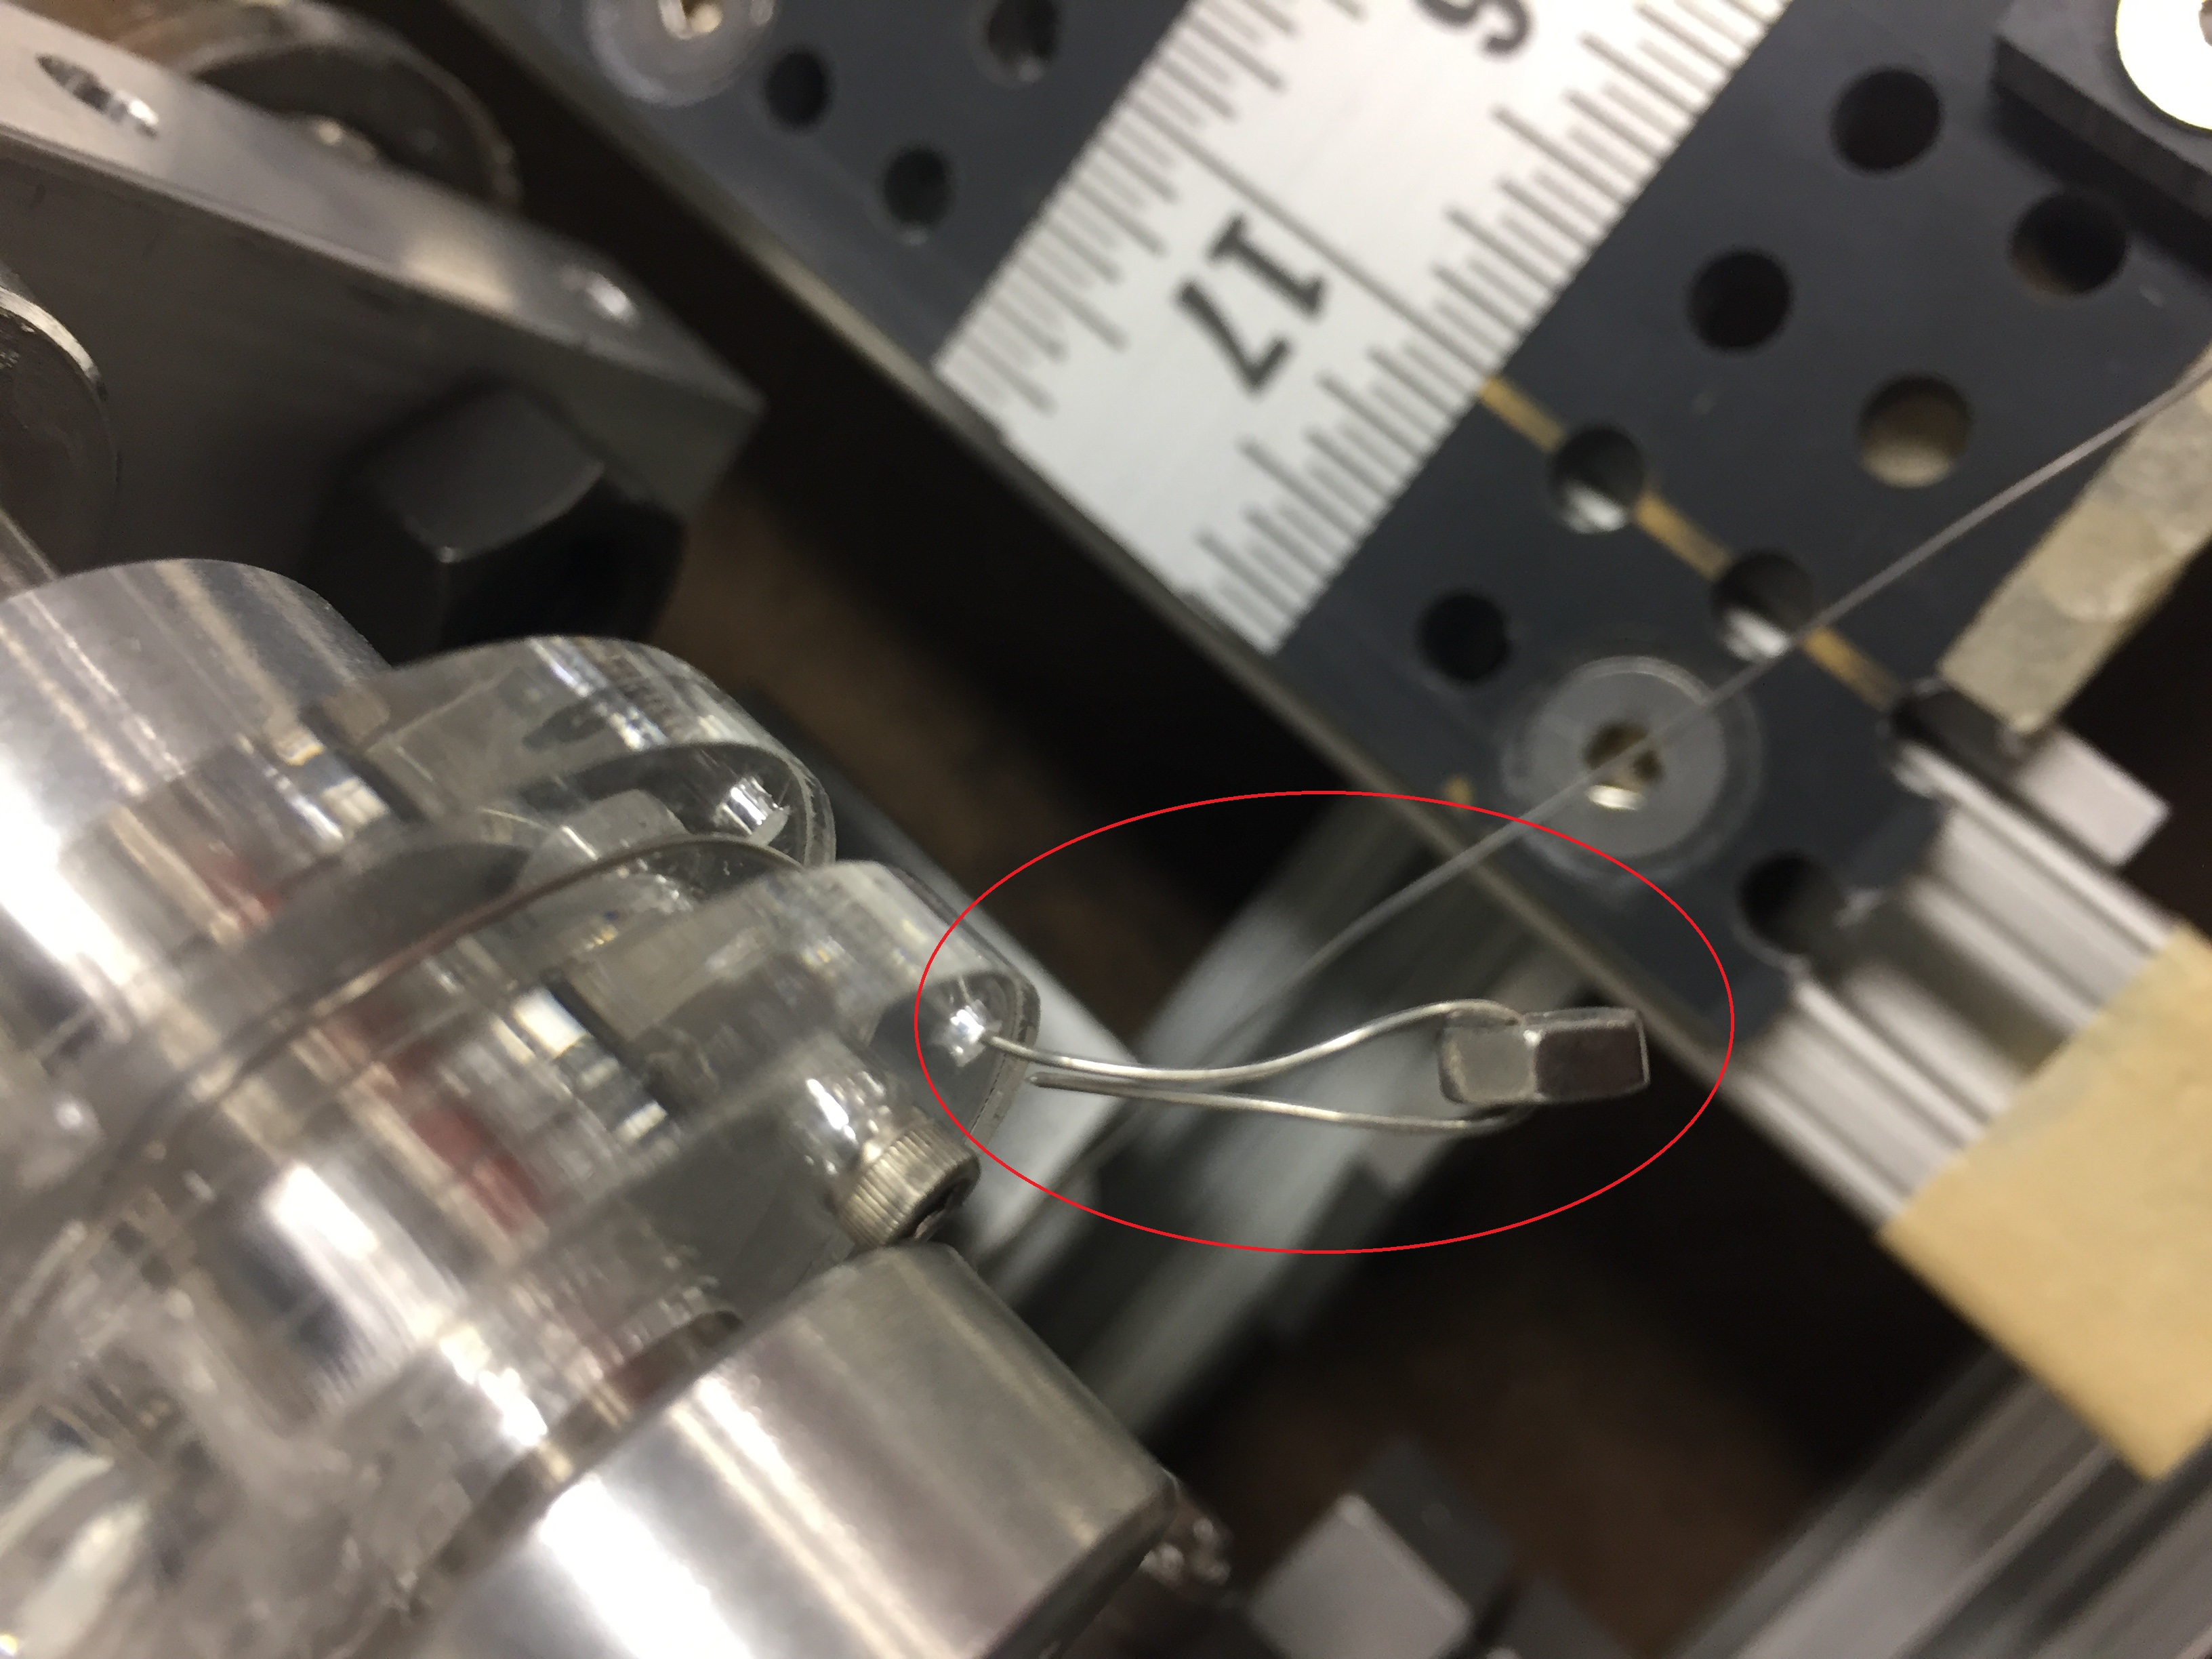
\includegraphics[width=\textwidth]{./Figures/Wire_mounting/8.jpg}
		\caption{Step 8}
	\end{subfigure}
	\caption{Steps 5-8}
\end{figure}

\item On the back side of the pulley, feed the wire around the copper sleeve bearing.
\item Feed the end of the wire through one of the small mounting holes on the acrylic pulley.
\item Remove the nut stored on the alligator clip.
\item Wrap the wire around the nut.

\begin{figure}[H]
	\centering
	\begin{subfigure}[b]{.475\textwidth}
		\centering
		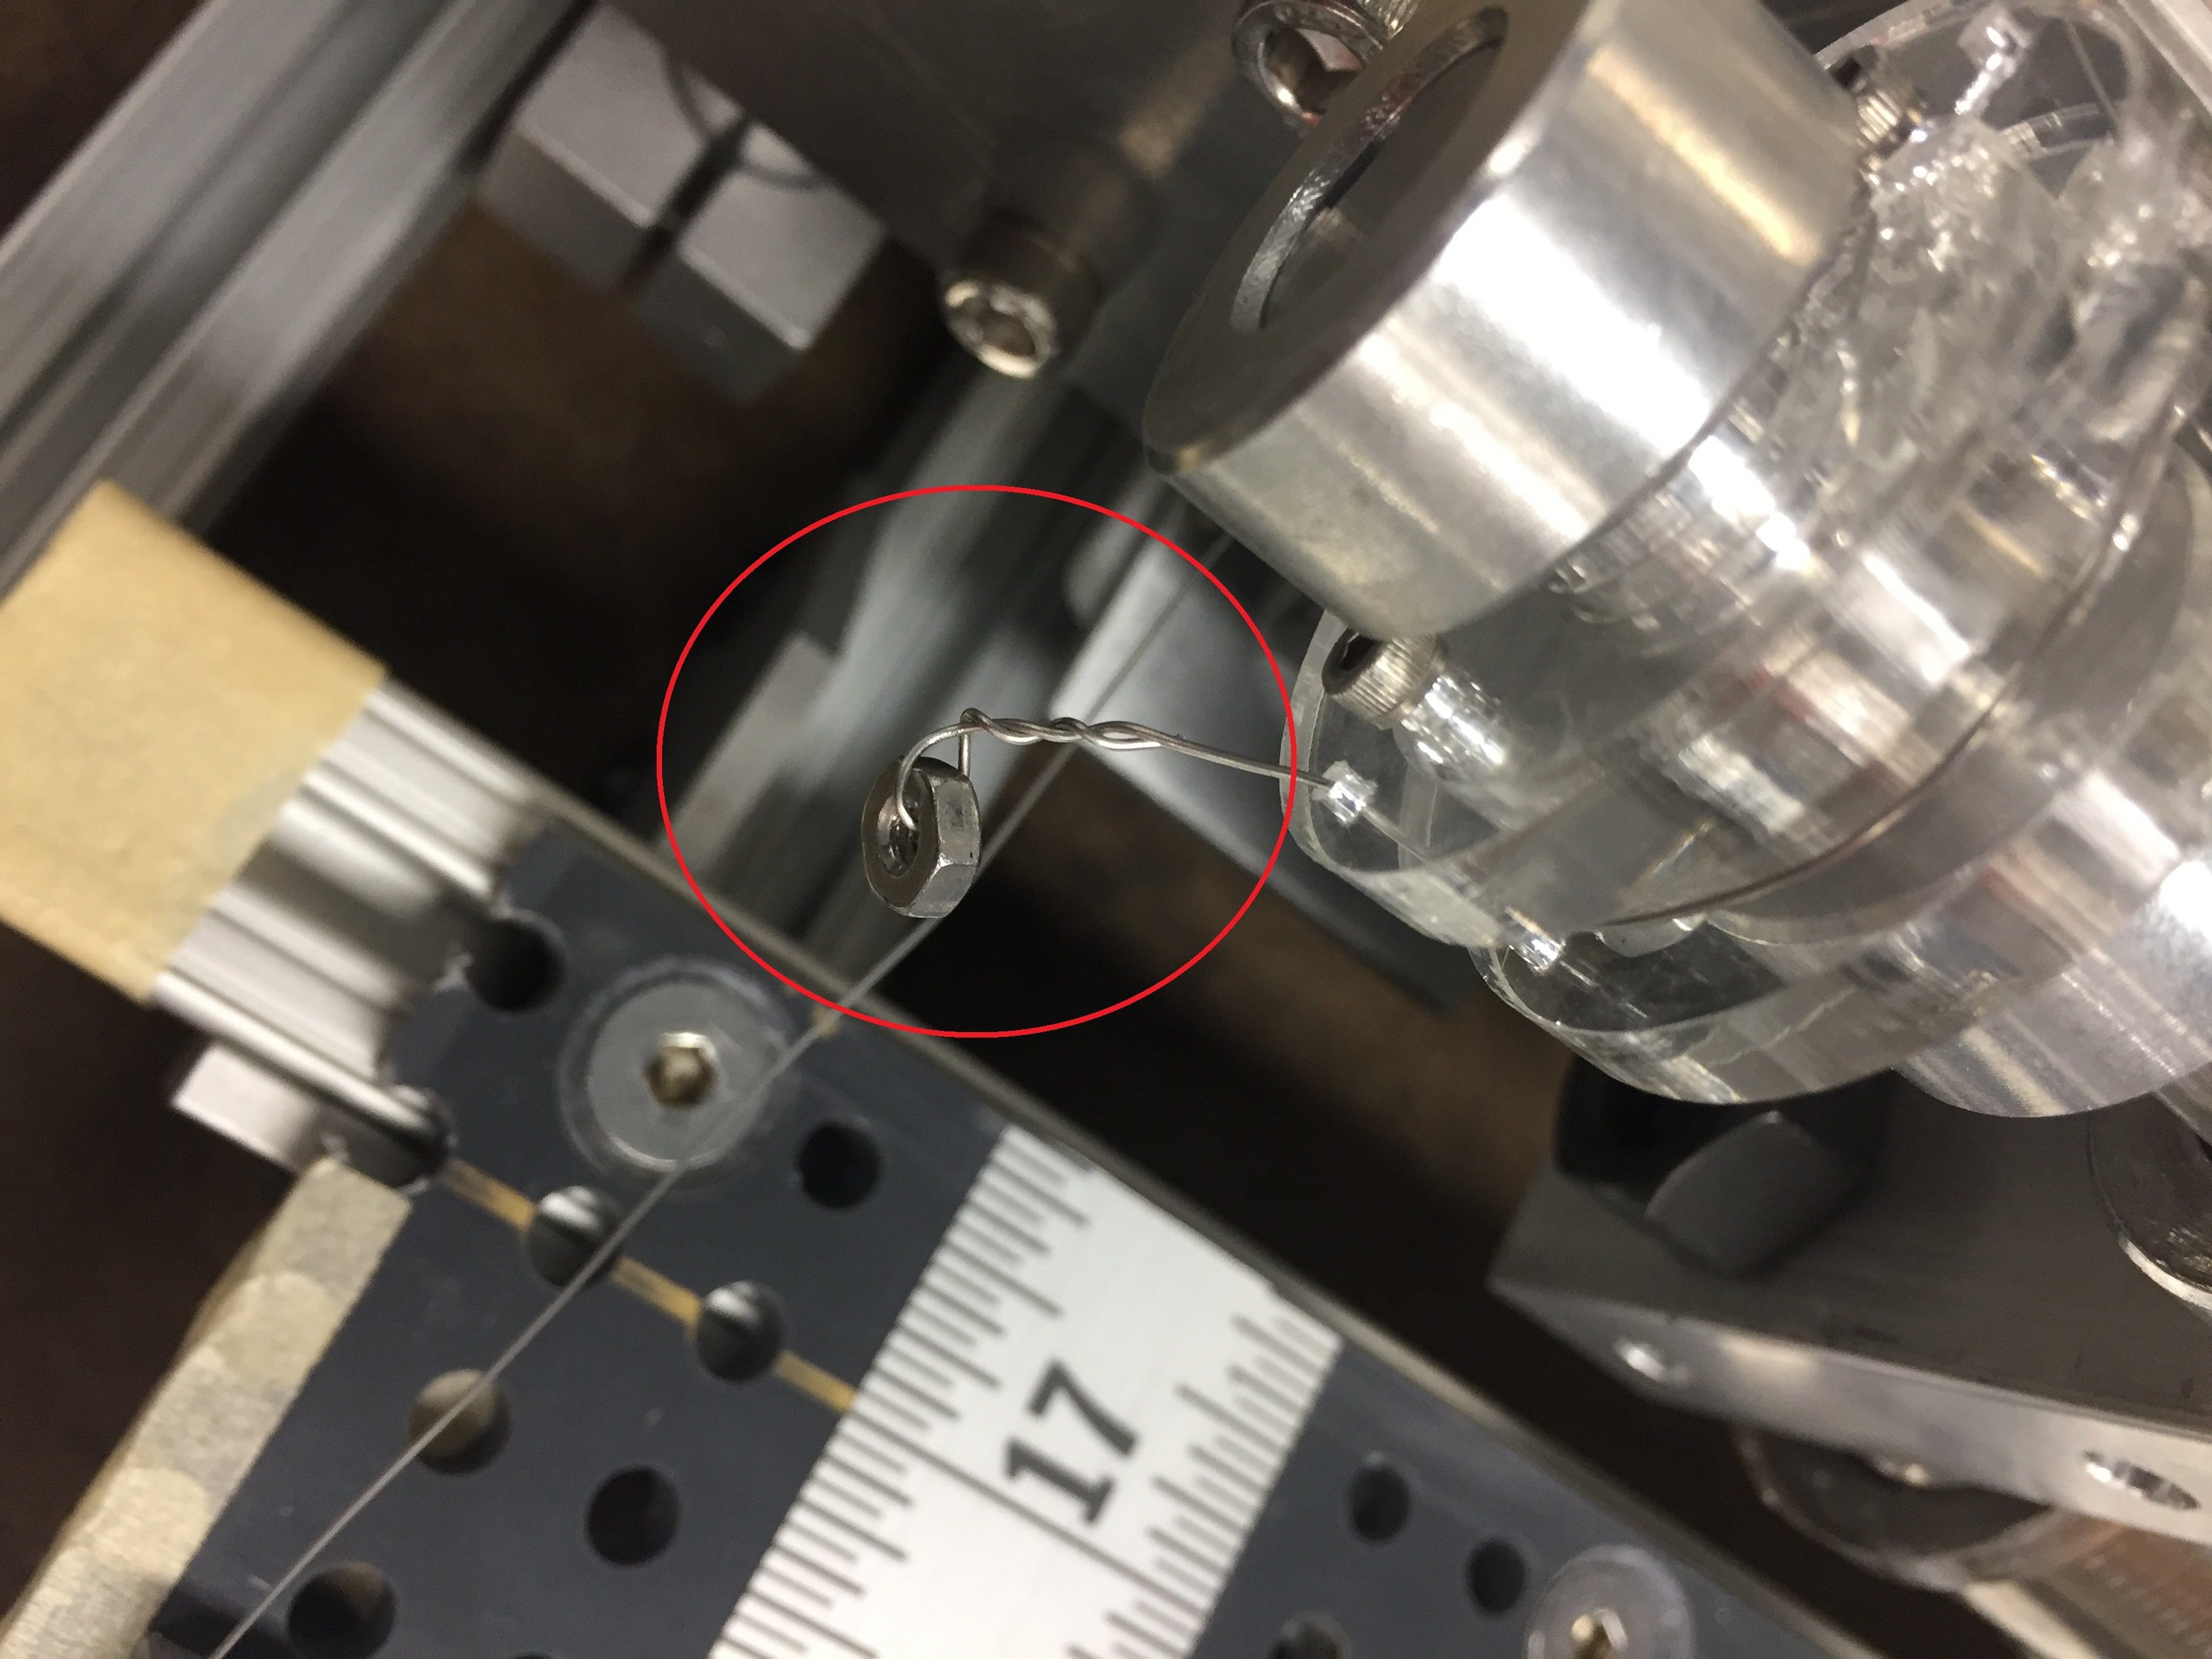
\includegraphics[width=\textwidth]{./Figures/Wire_mounting/9.jpg}
		\caption{Step 9}
	\end{subfigure}
	\begin{subfigure}[b]{.475\textwidth}
		\centering
		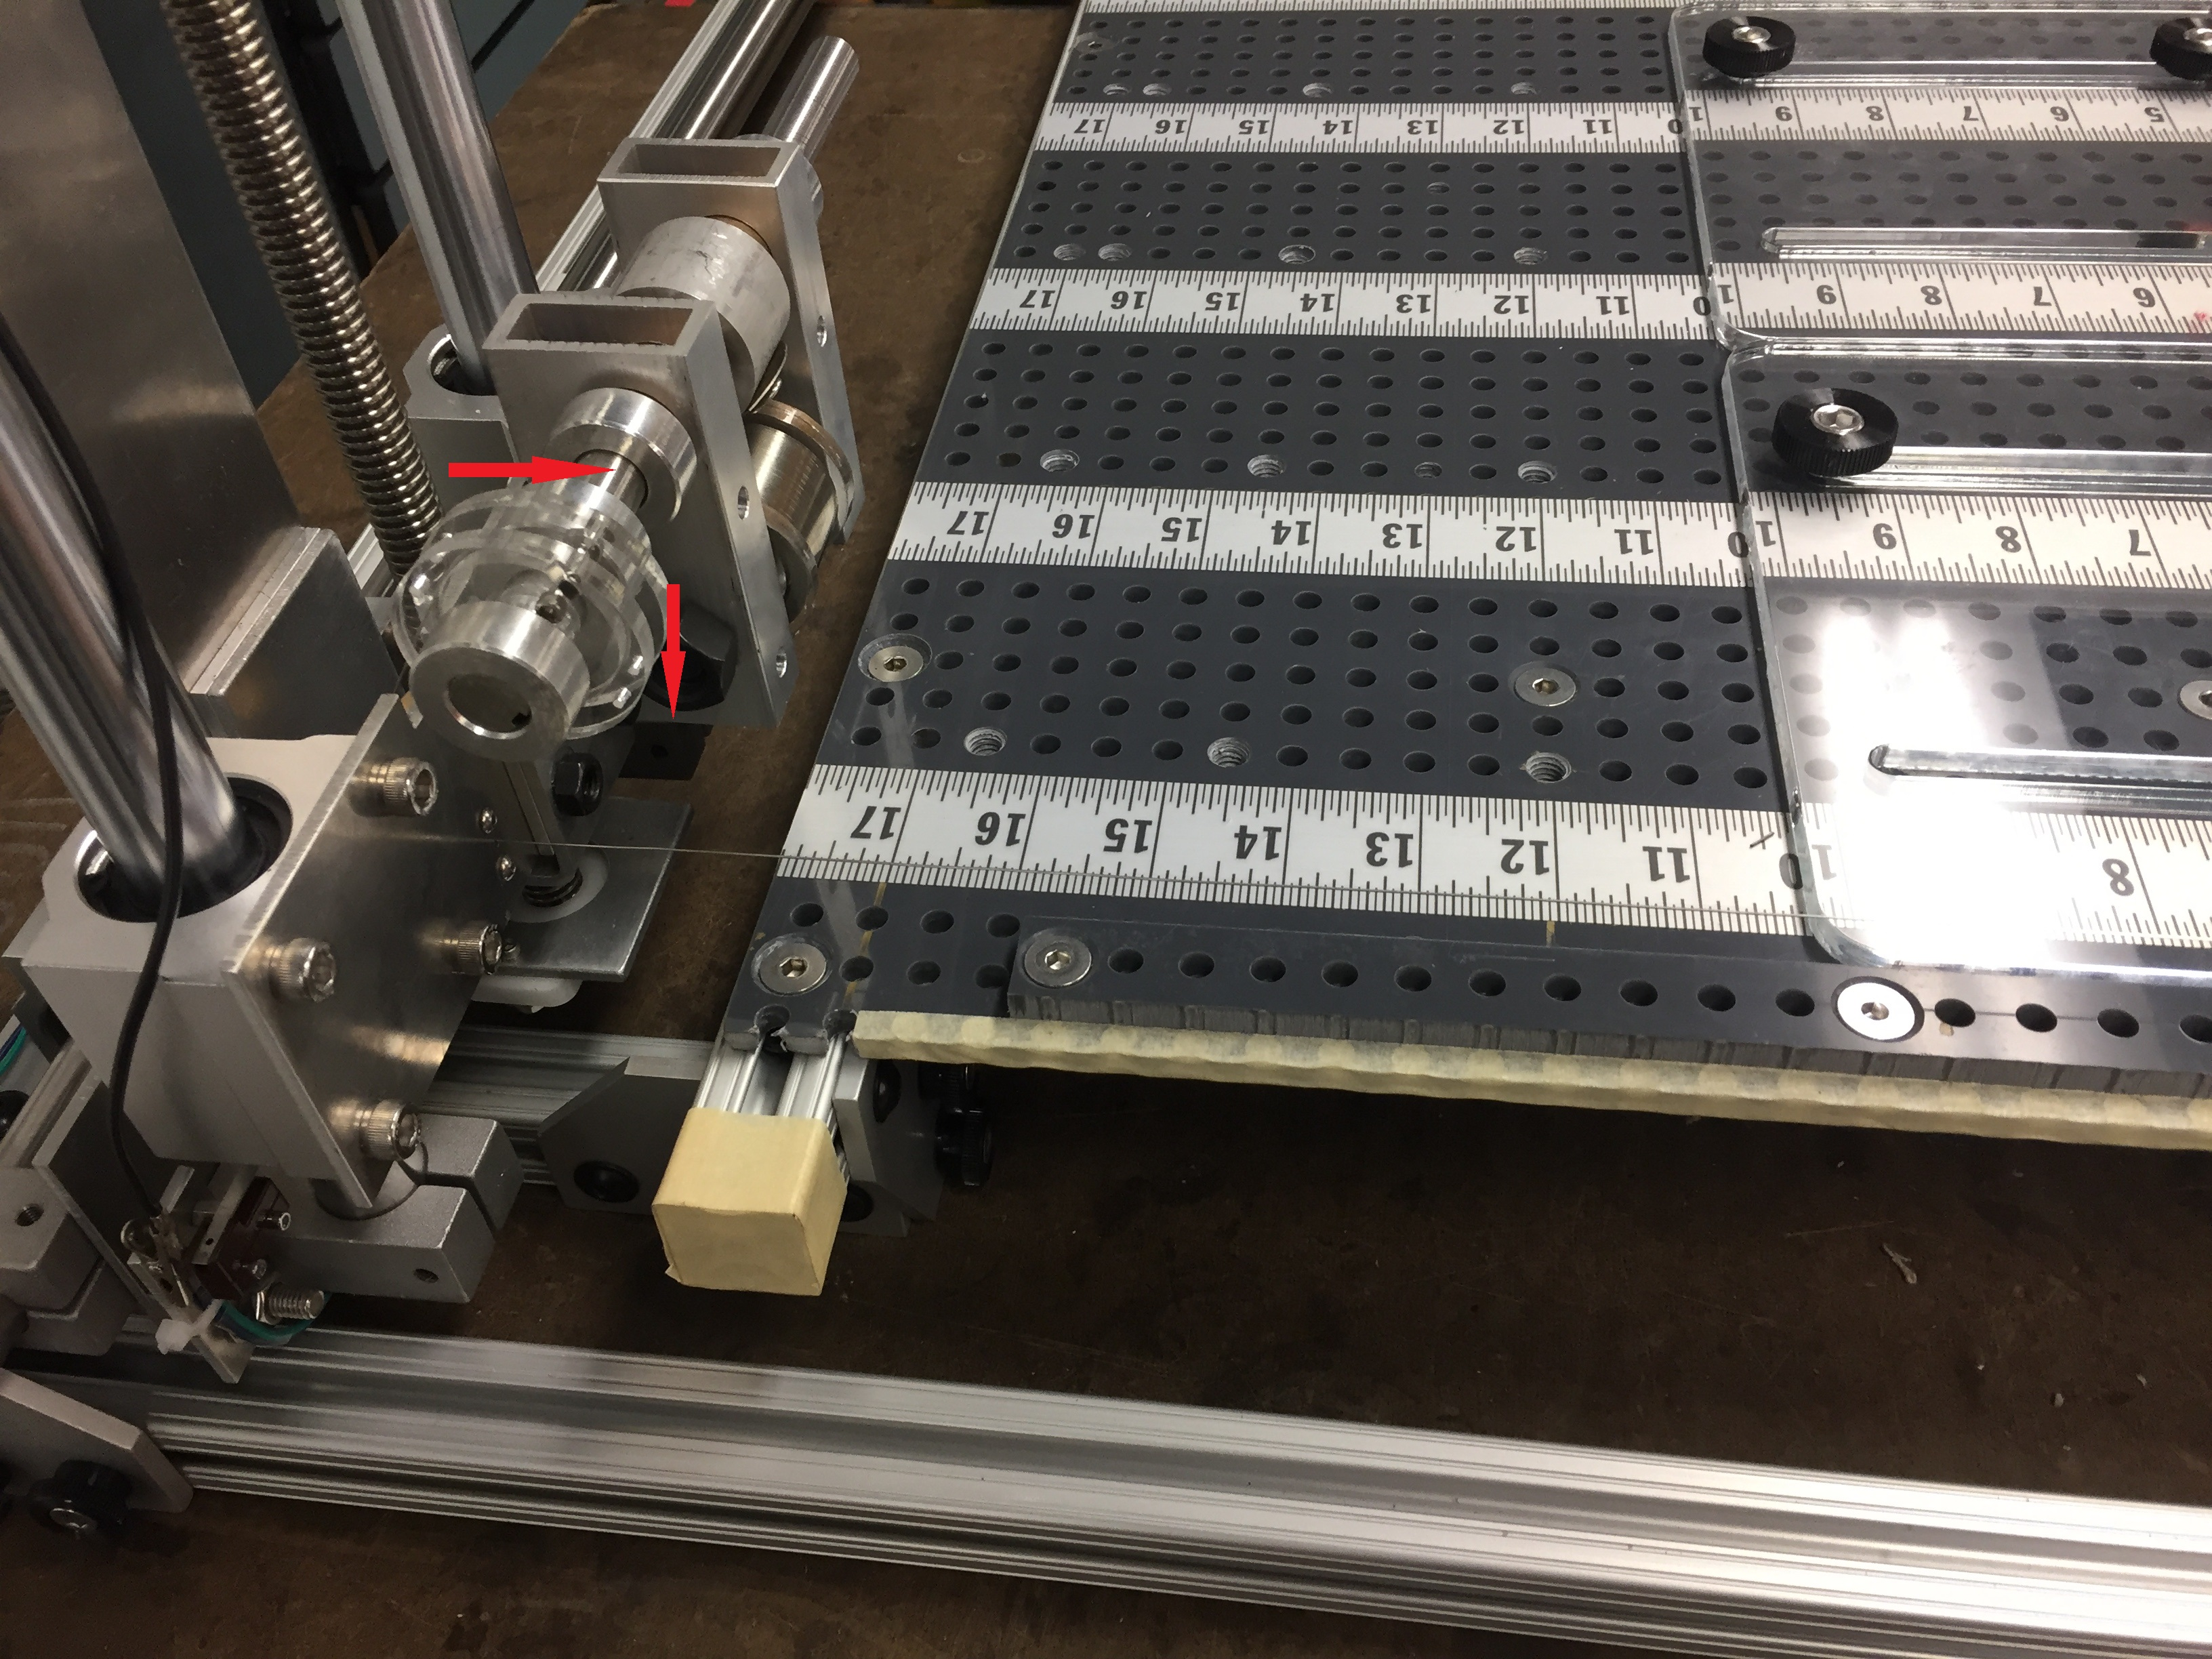
\includegraphics[width=\textwidth]{./Figures/Wire_mounting/10.jpg}
		\caption{Step 10}
	\end{subfigure}
	\centering
	\begin{subfigure}[b]{.475\textwidth}
		\centering
		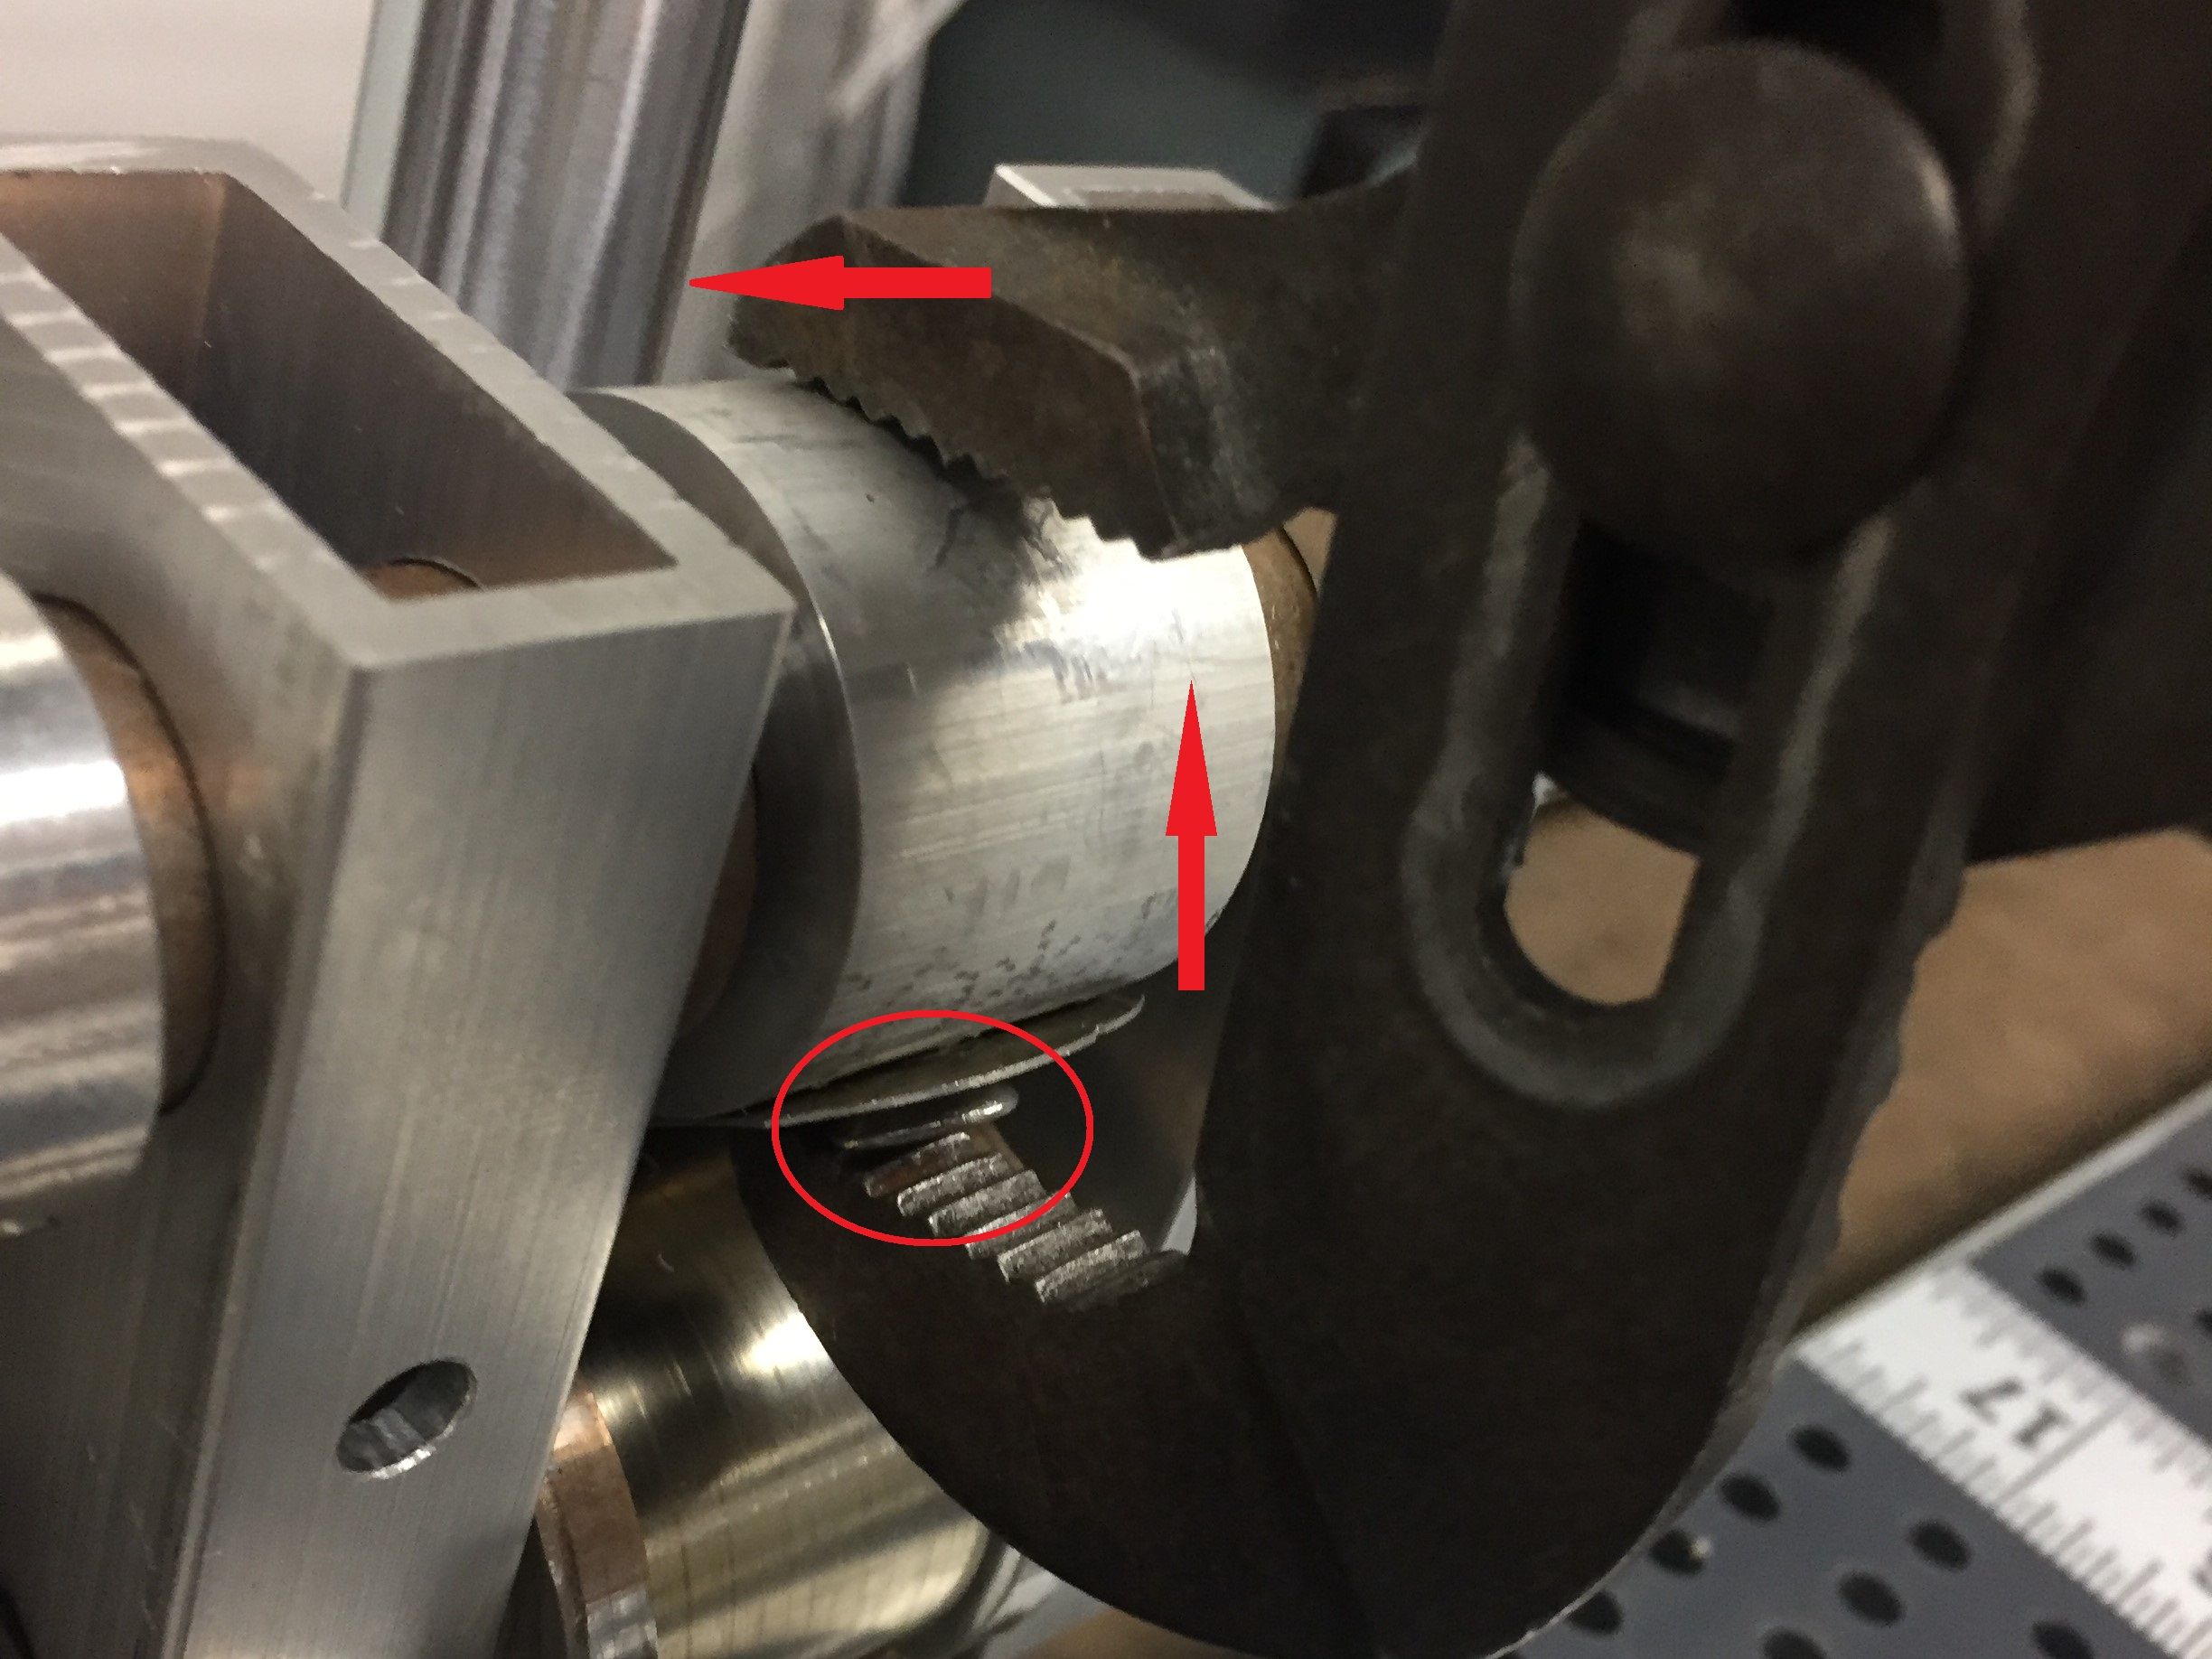
\includegraphics[width=\textwidth]{./Figures/Wire_mounting/11.jpg}
		\caption{Step 11}
	\end{subfigure}
	\begin{subfigure}[b]{.475\textwidth}
		\centering
		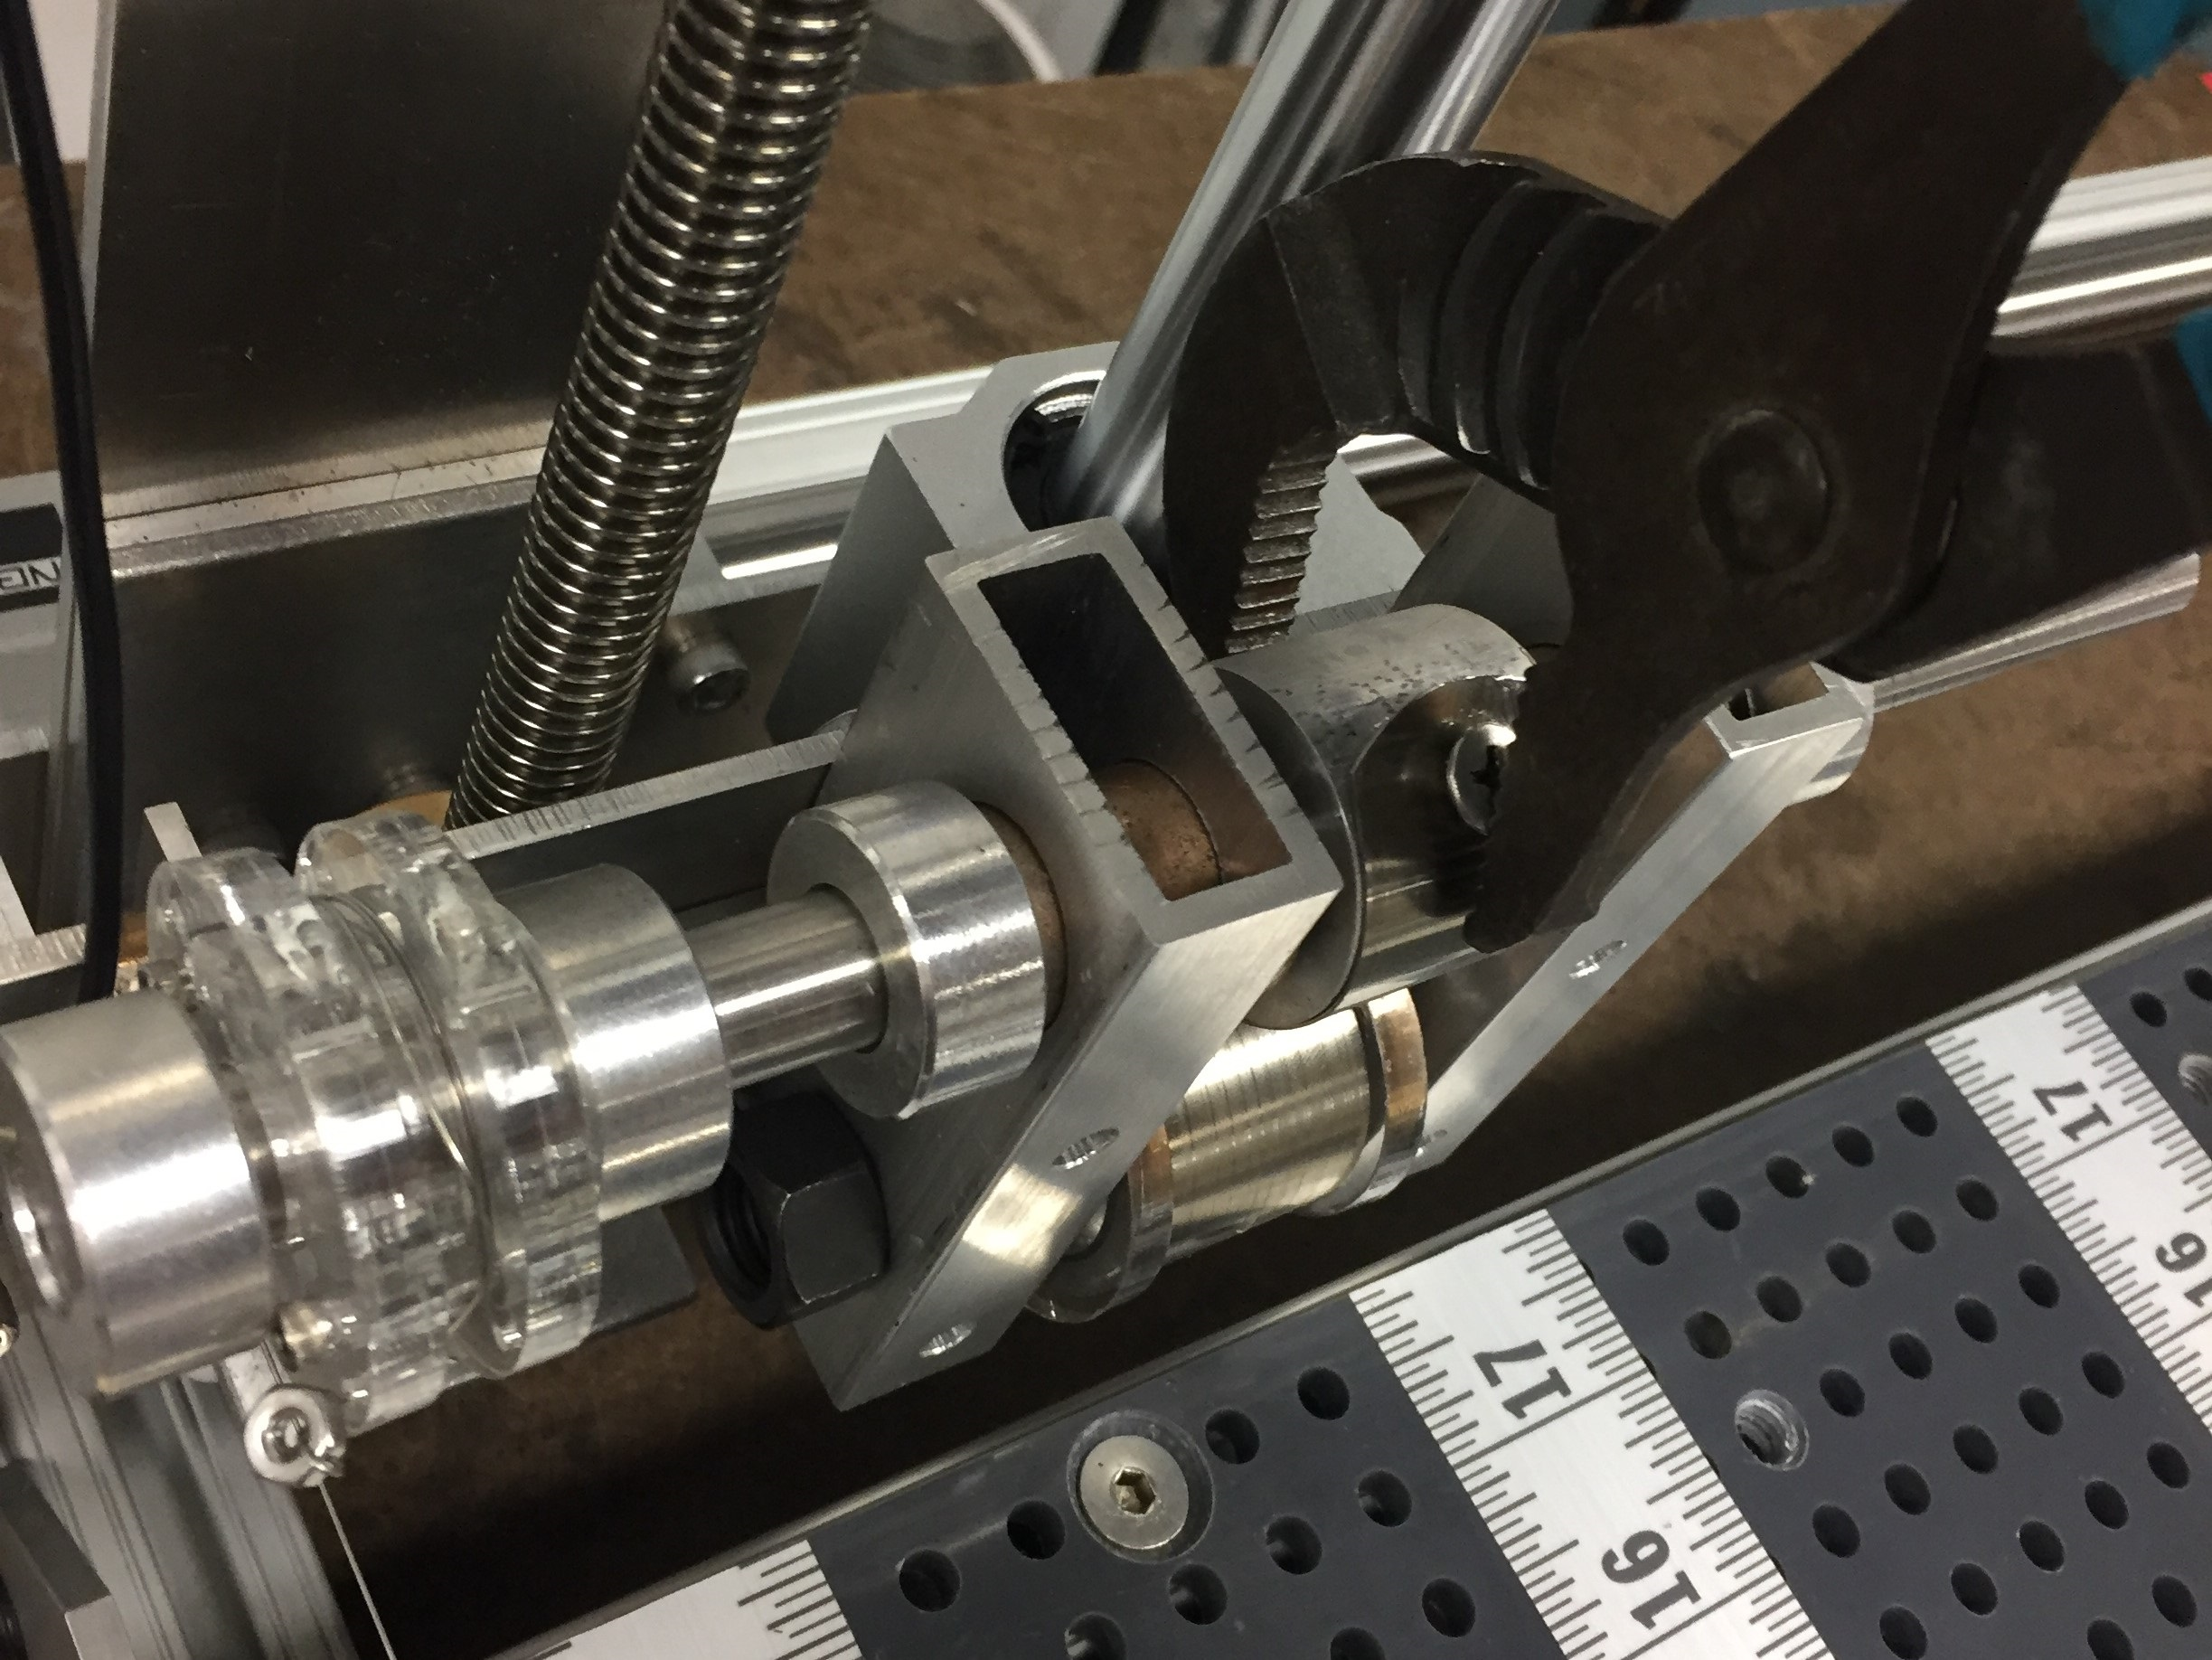
\includegraphics[width=\textwidth]{./Figures/Wire_mounting/12.jpg}
		\caption{Step 12}
	\end{subfigure}	
	\centering
	\begin{subfigure}[b]{.475\textwidth}
		\centering
		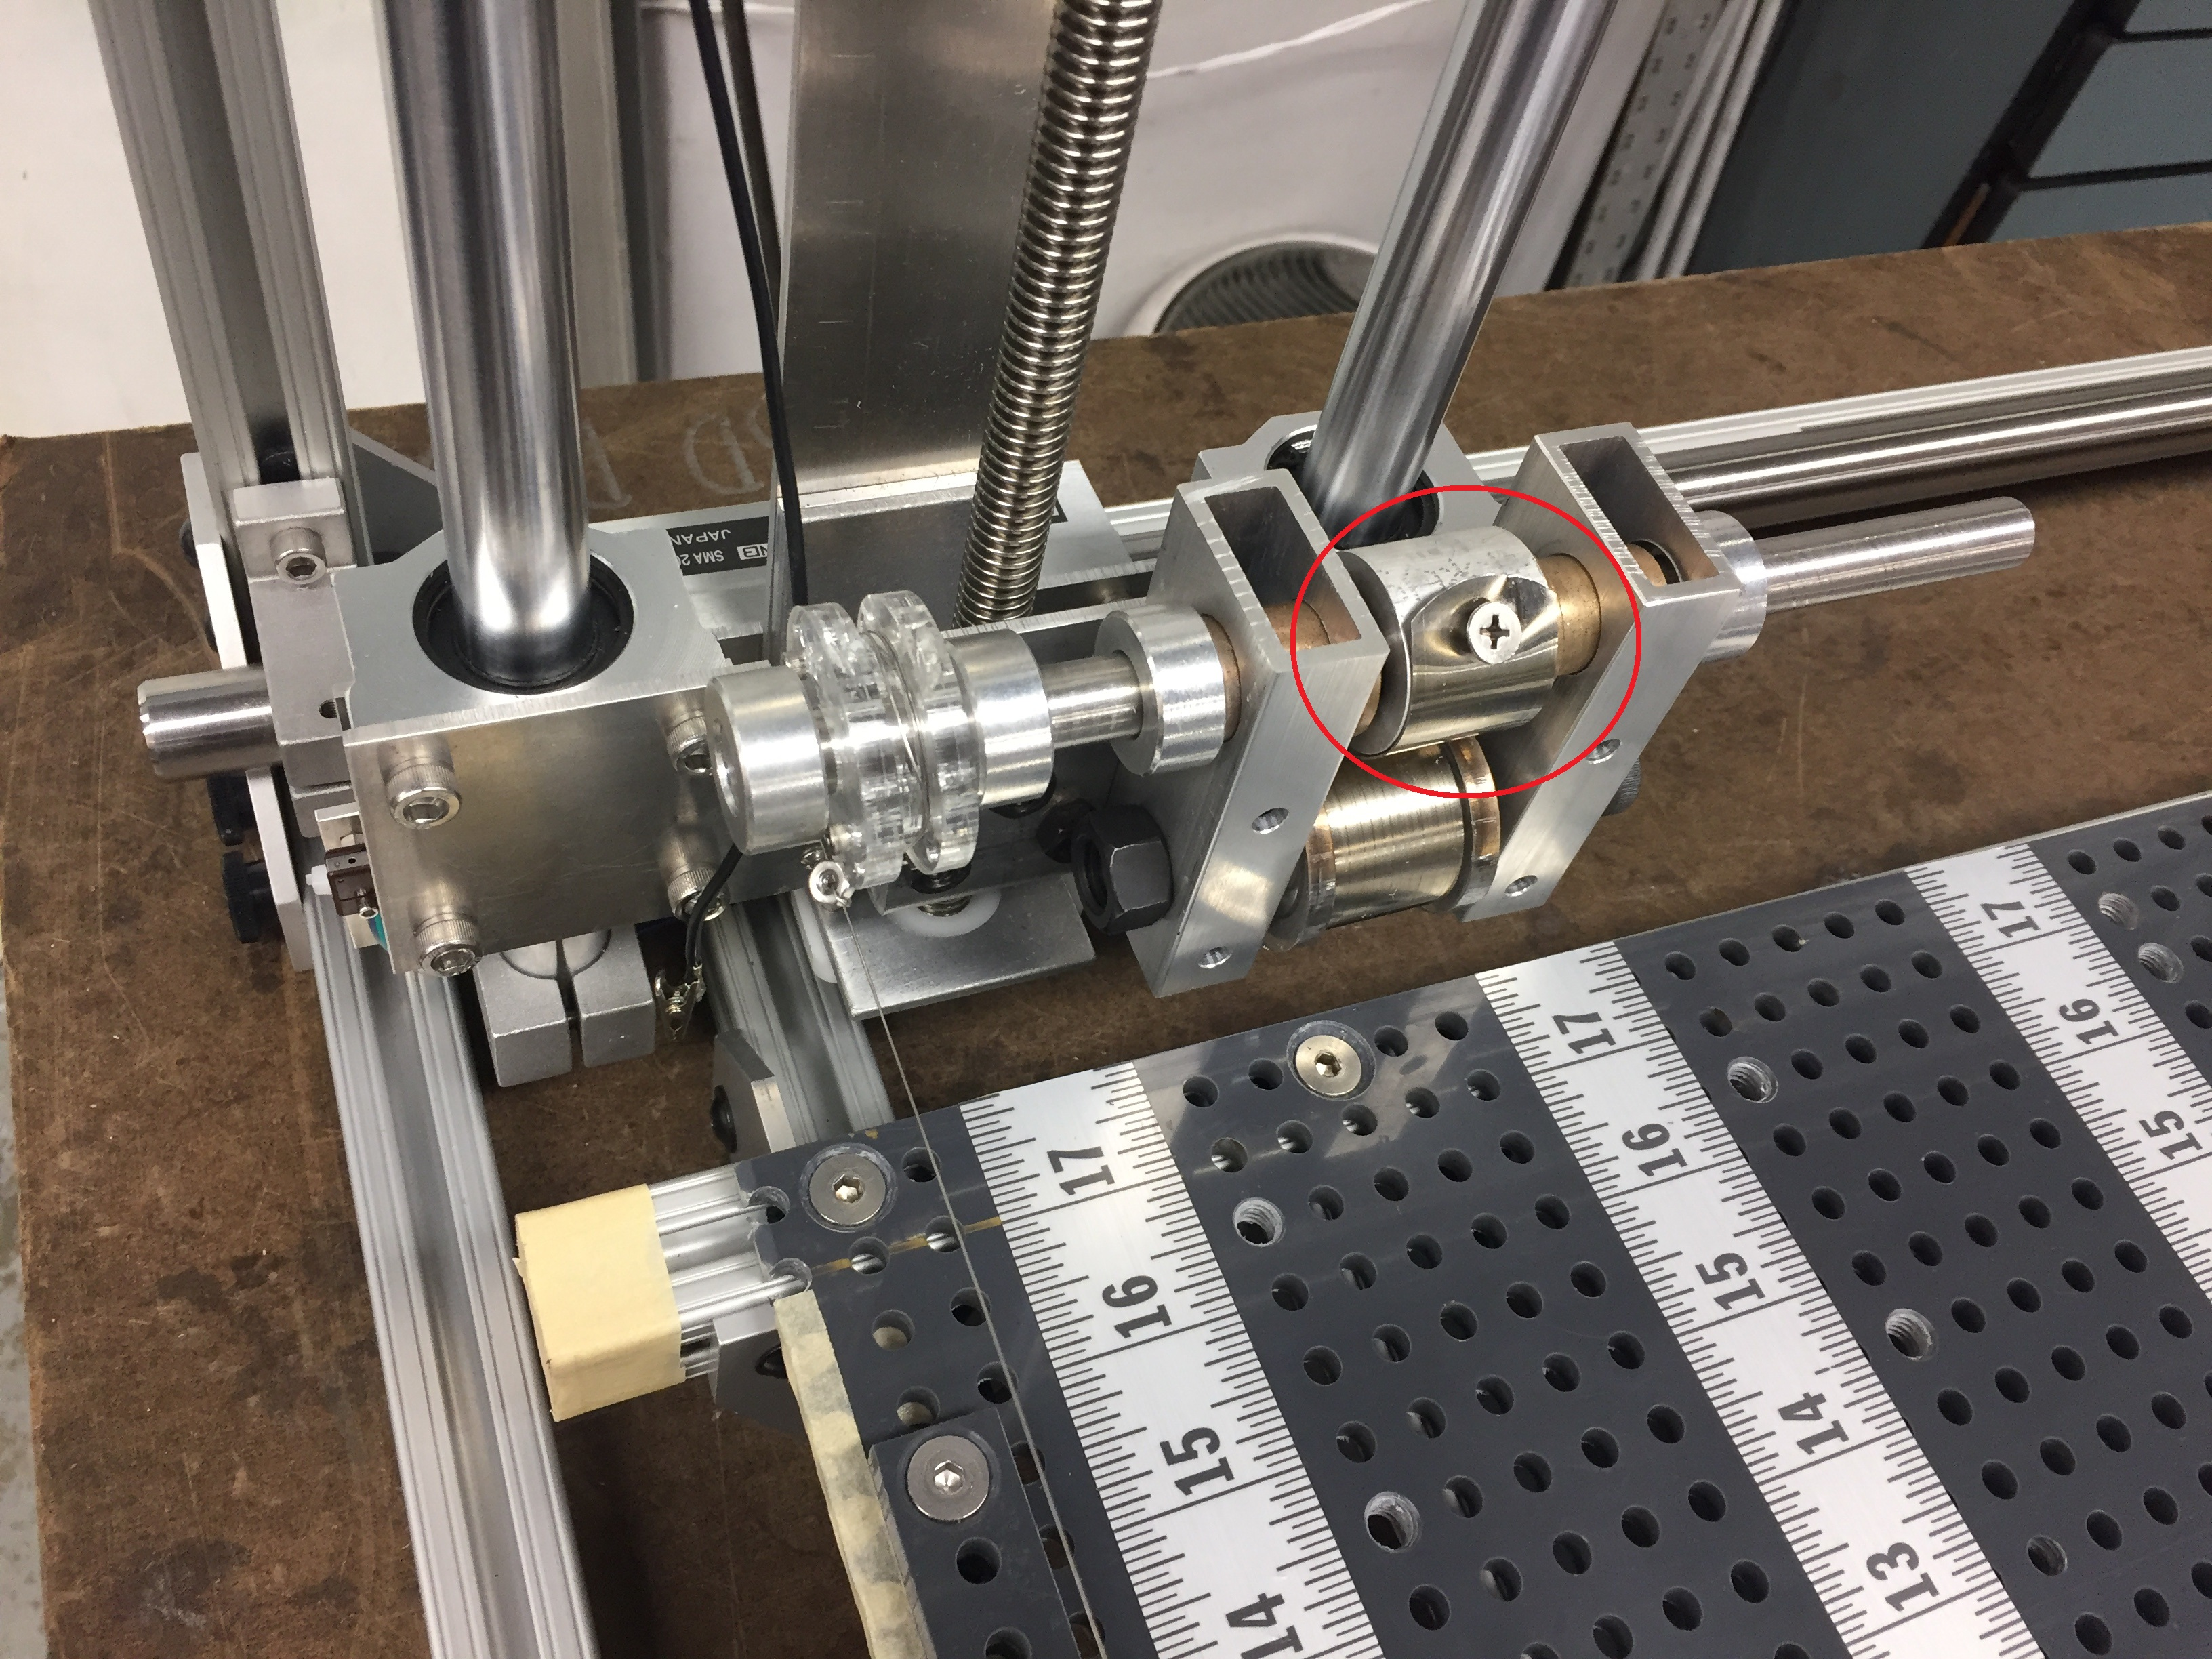
\includegraphics[width=\textwidth]{./Figures/Wire_mounting/13.jpg}
		\caption{Step 13}
	\end{subfigure}
	\begin{subfigure}[b]{.475\textwidth}
		\centering
		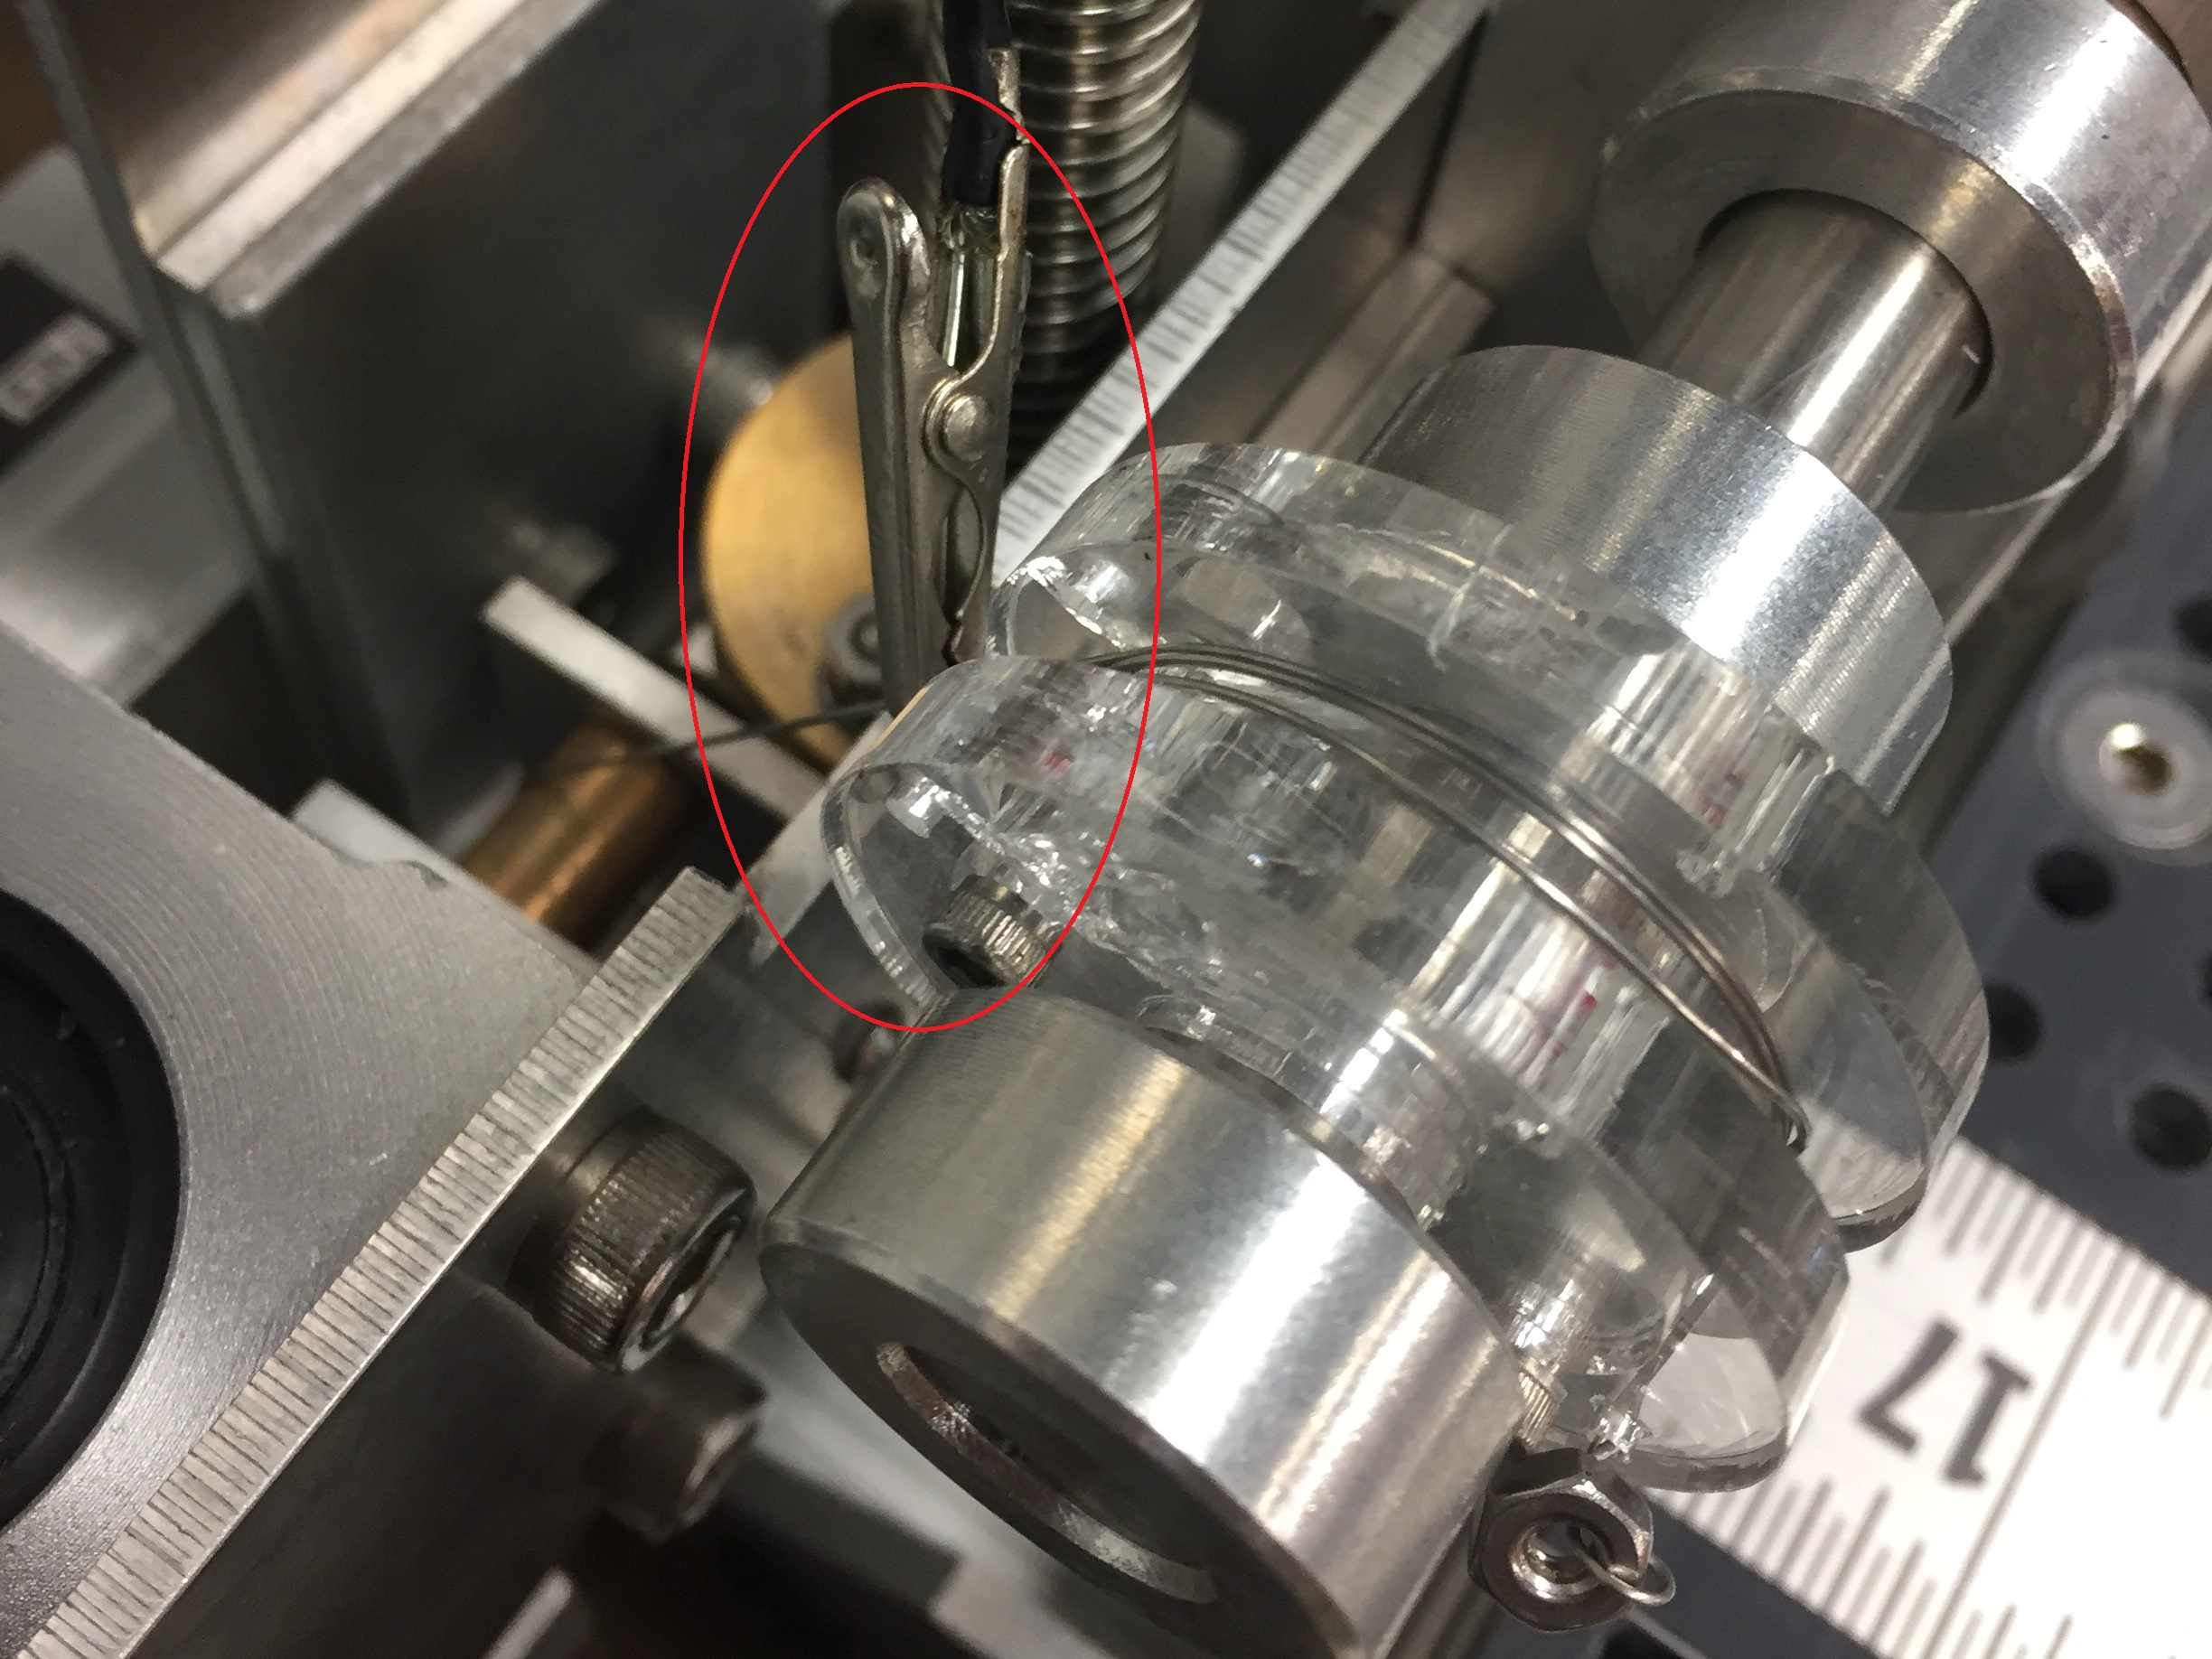
\includegraphics[width=\textwidth]{./Figures/Wire_mounting/14.jpg}
		\caption{Step 14}
	\end{subfigure}
	\caption{Steps 9-12}
\end{figure}
\item Twist the wire around the nut.
\item Rotate the acrylic pulley clockwise to tighten the wire.
\item Hold the acrylic pulley by hand. Use a wrench to further tighten the spring by holding onto the mounting screw of the spring and rotate counterclockwise.
\item Further tighten the spring with the wrench.
\item Tighten the spring to the approximate position shown in the figure.
\item Clip the alligator click next to the pulley. On the other end, clip the other alligator clip on the back side of the guiding hole, and \textbf{make sure the alligator clip does not touch anything other than the hot wire.}
\end{enumerate}

\section{Foamcutter Software Setup}
\subsection{Connect to the Pi}
\begin{enumerate}[itemsep = 5pt,topsep=0pt]
	\item Perform the Laptop setup guide in Chapter 1 Section~\ref{sec:laptop} if not already completed.
	\item Plug in the power cord to the foamcutter to power on the Pi.
	\item Connect to the WiFi hotspot named \textbf{``foamcutter''} with password \textbf{``ucsdaiaadbf''}.
	\item SSH into the Pi by opening PuTTY and double click on the saved session named \textbf{``foamcutter''}. Enter the user name \textbf{``pi''} then password \textbf{``ucsdaiaadbf''}.
	\item Open WinSCP, a window similar to fig~\ref{fig:winscp} below should show up. The left hand side are folders and files on your computer, while the right hand side is files on the Pi. Make sure the right hand side is in the folder \textbf{``/home/pi''}, if not, navigate to it. To create new folder on the Pi, use the \textbf{``new directory''} button. To upload files from your computer to the Pi, simply drag the file/folder from the left half to the right half. 
	\begin{figure} [H]
		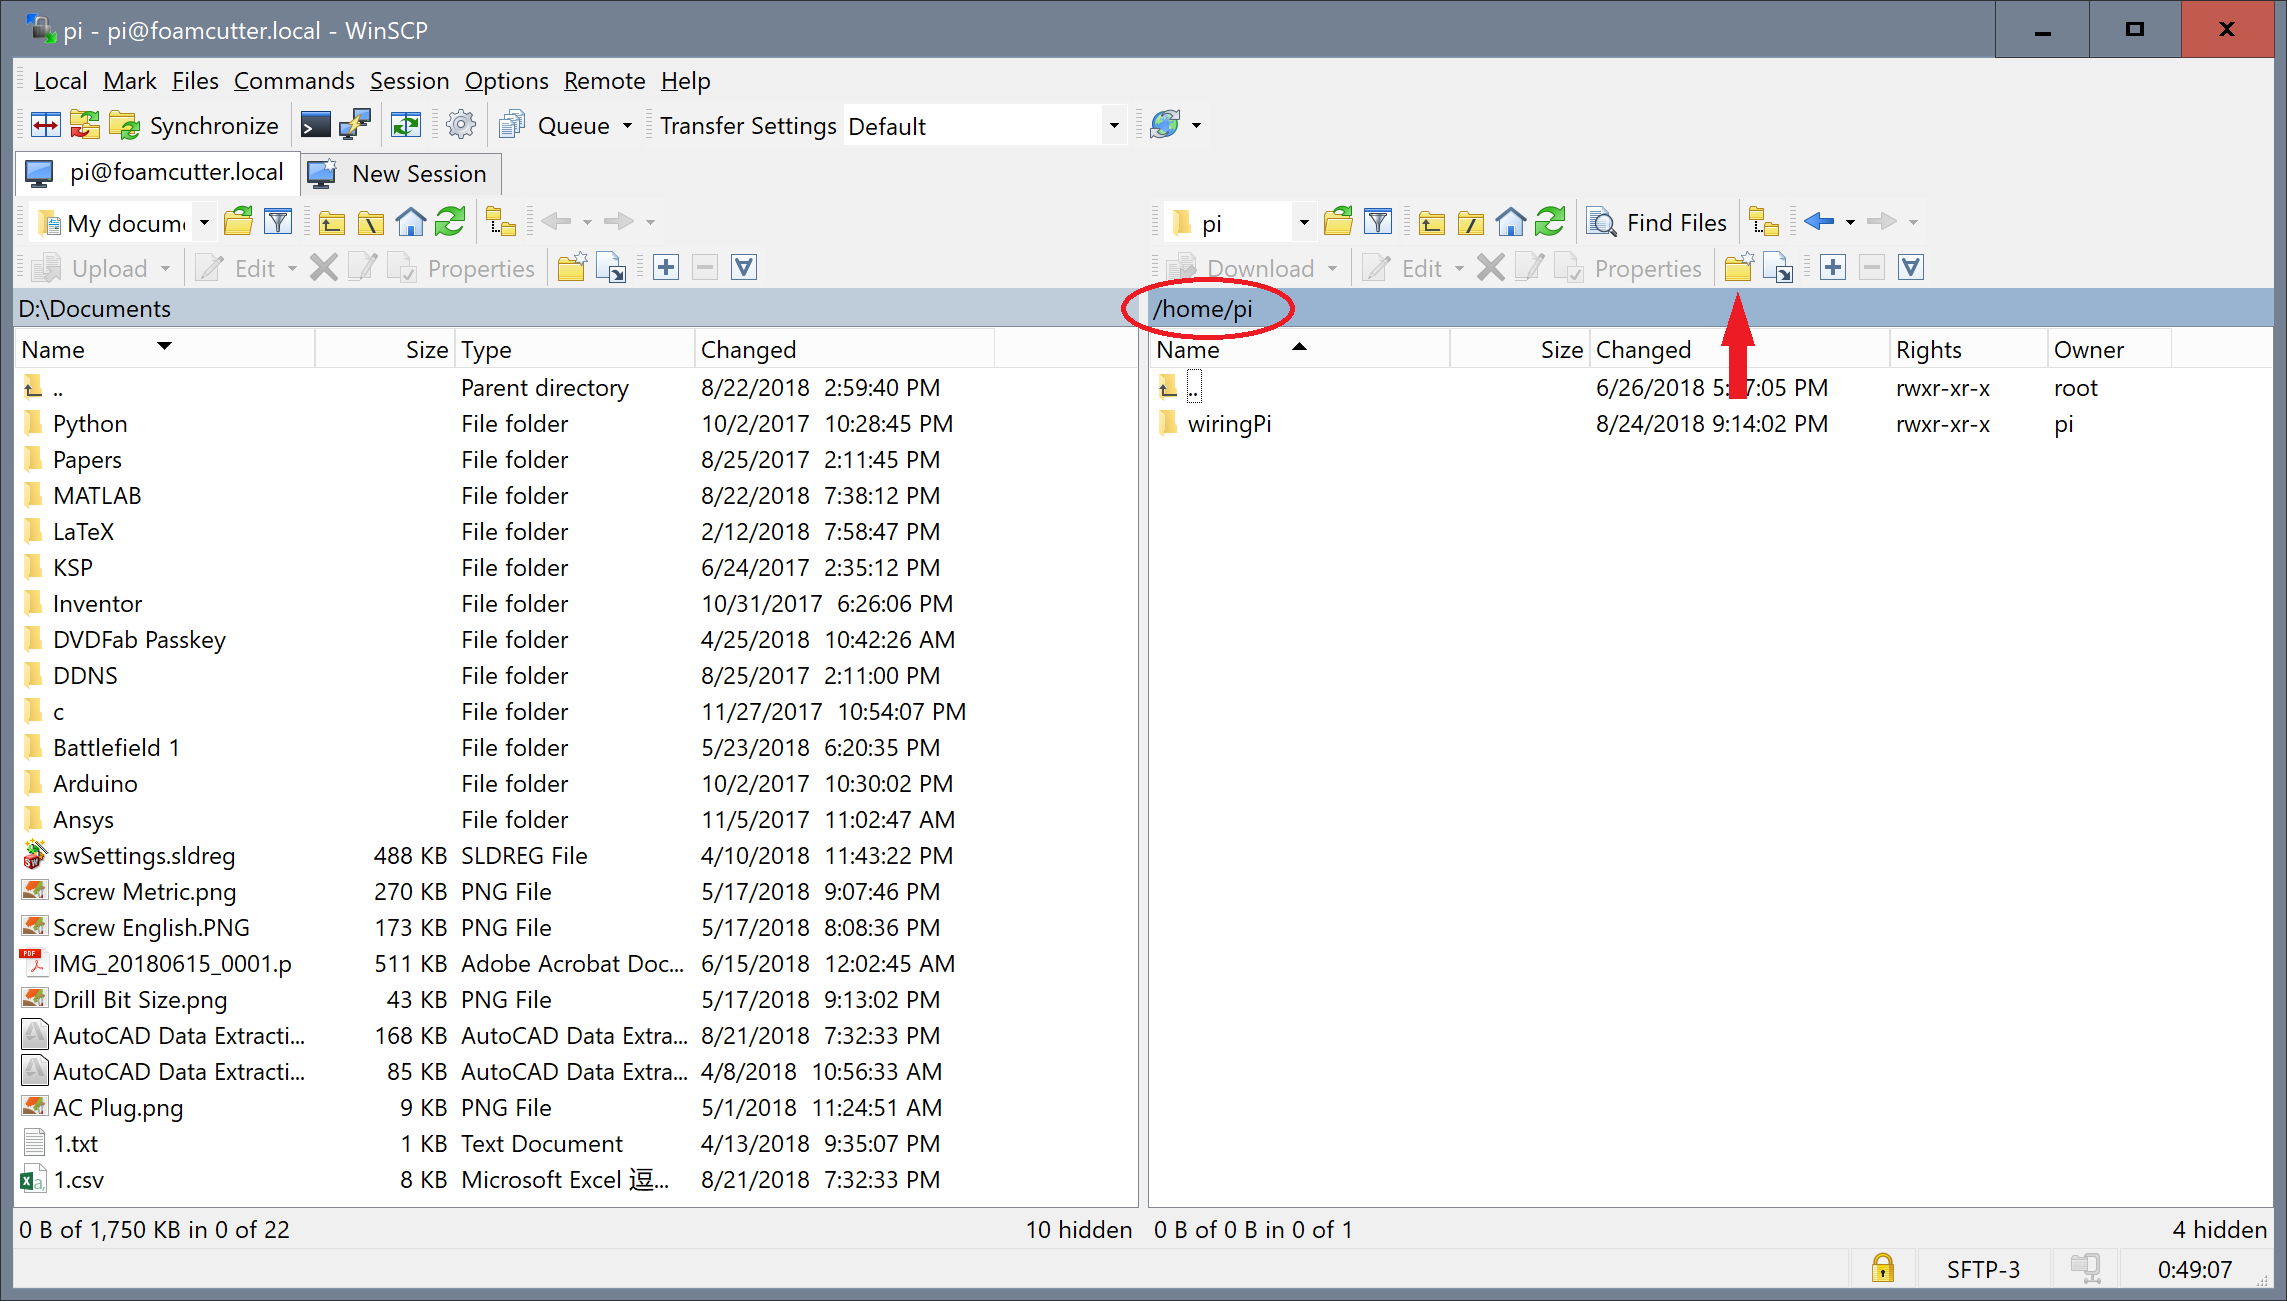
\includegraphics[width = 0.9\linewidth]{./Figures/winscp.png}
		\caption{WinSCP Window}
		\label{fig:winscp}
	\end{figure}
\end{enumerate}

\subsection{Install/Update the Foamcutter Software and Calibrate Wire Origin}
\label{sec:calibration}
The 4 axes of the foamcutter each have one limit switch installed. Upon starting of the program, the foamcutter moves all axes towards the negative direction until hitting the limit switches. Then the foamcutter moves the 4 axes each a distance specified in the setting file to reach the Origin. \textbf{This calibration only needs to be performed once in a while to improve accuracy.} Please follow the  steps to calibrate the wire origin:

\begin{enumerate}[itemsep = 5pt,topsep=0pt]
\item Download the \textbf{``User Package.zip''} from \href{https://github.com/ythuang96/FoamCutter}{https://github.com/ythuang96/FoamCutter}, and unzip it.
\item In WinSCP, create a new folder on the Pi called \textbf{``foamcutter''} in the directory of \textbf{``/home/pi''}. 
\item In WinSCP, upload the files named \textbf{``foamcutter.c''}, \textbf{``foamcutter\_setup.h''} and \textbf{``Makefile''} from the \textbf{''User Package''} just downloaded into the \textbf{``foamcutter''} folder just created on the Pi.
\item In PuTTY, run the following commands line by line:
\begin{itemize}[noitemsep,topsep=0pt]
	\item \textbf{cd}
	\item \textbf{cd foamcutter}
	\item \textbf{make foamcutter}
	\item \textbf{sudo ./foamcutter}
\end{itemize}
This will launch the foamcutter program.
\item In PuTTY, when the program reads \textbf{``I see the system is not homed yet, please press ENTER to home the system:''} press the Enter key. The foamcutter will move all 4 axes towards the negative direction until touching the limit switch. Then all 4 axes will move towards the positive direction to the origin.
\item Place a Aluminum block on the work panel against the work panel guiding block, and observe from top down as shown in fig~\ref{fig:zero1} below. Both the far left and far right of the wire should sit right against the aluminum block, measure the amount that needs to be adjusted in millimeters. 
\begin{figure} [H]
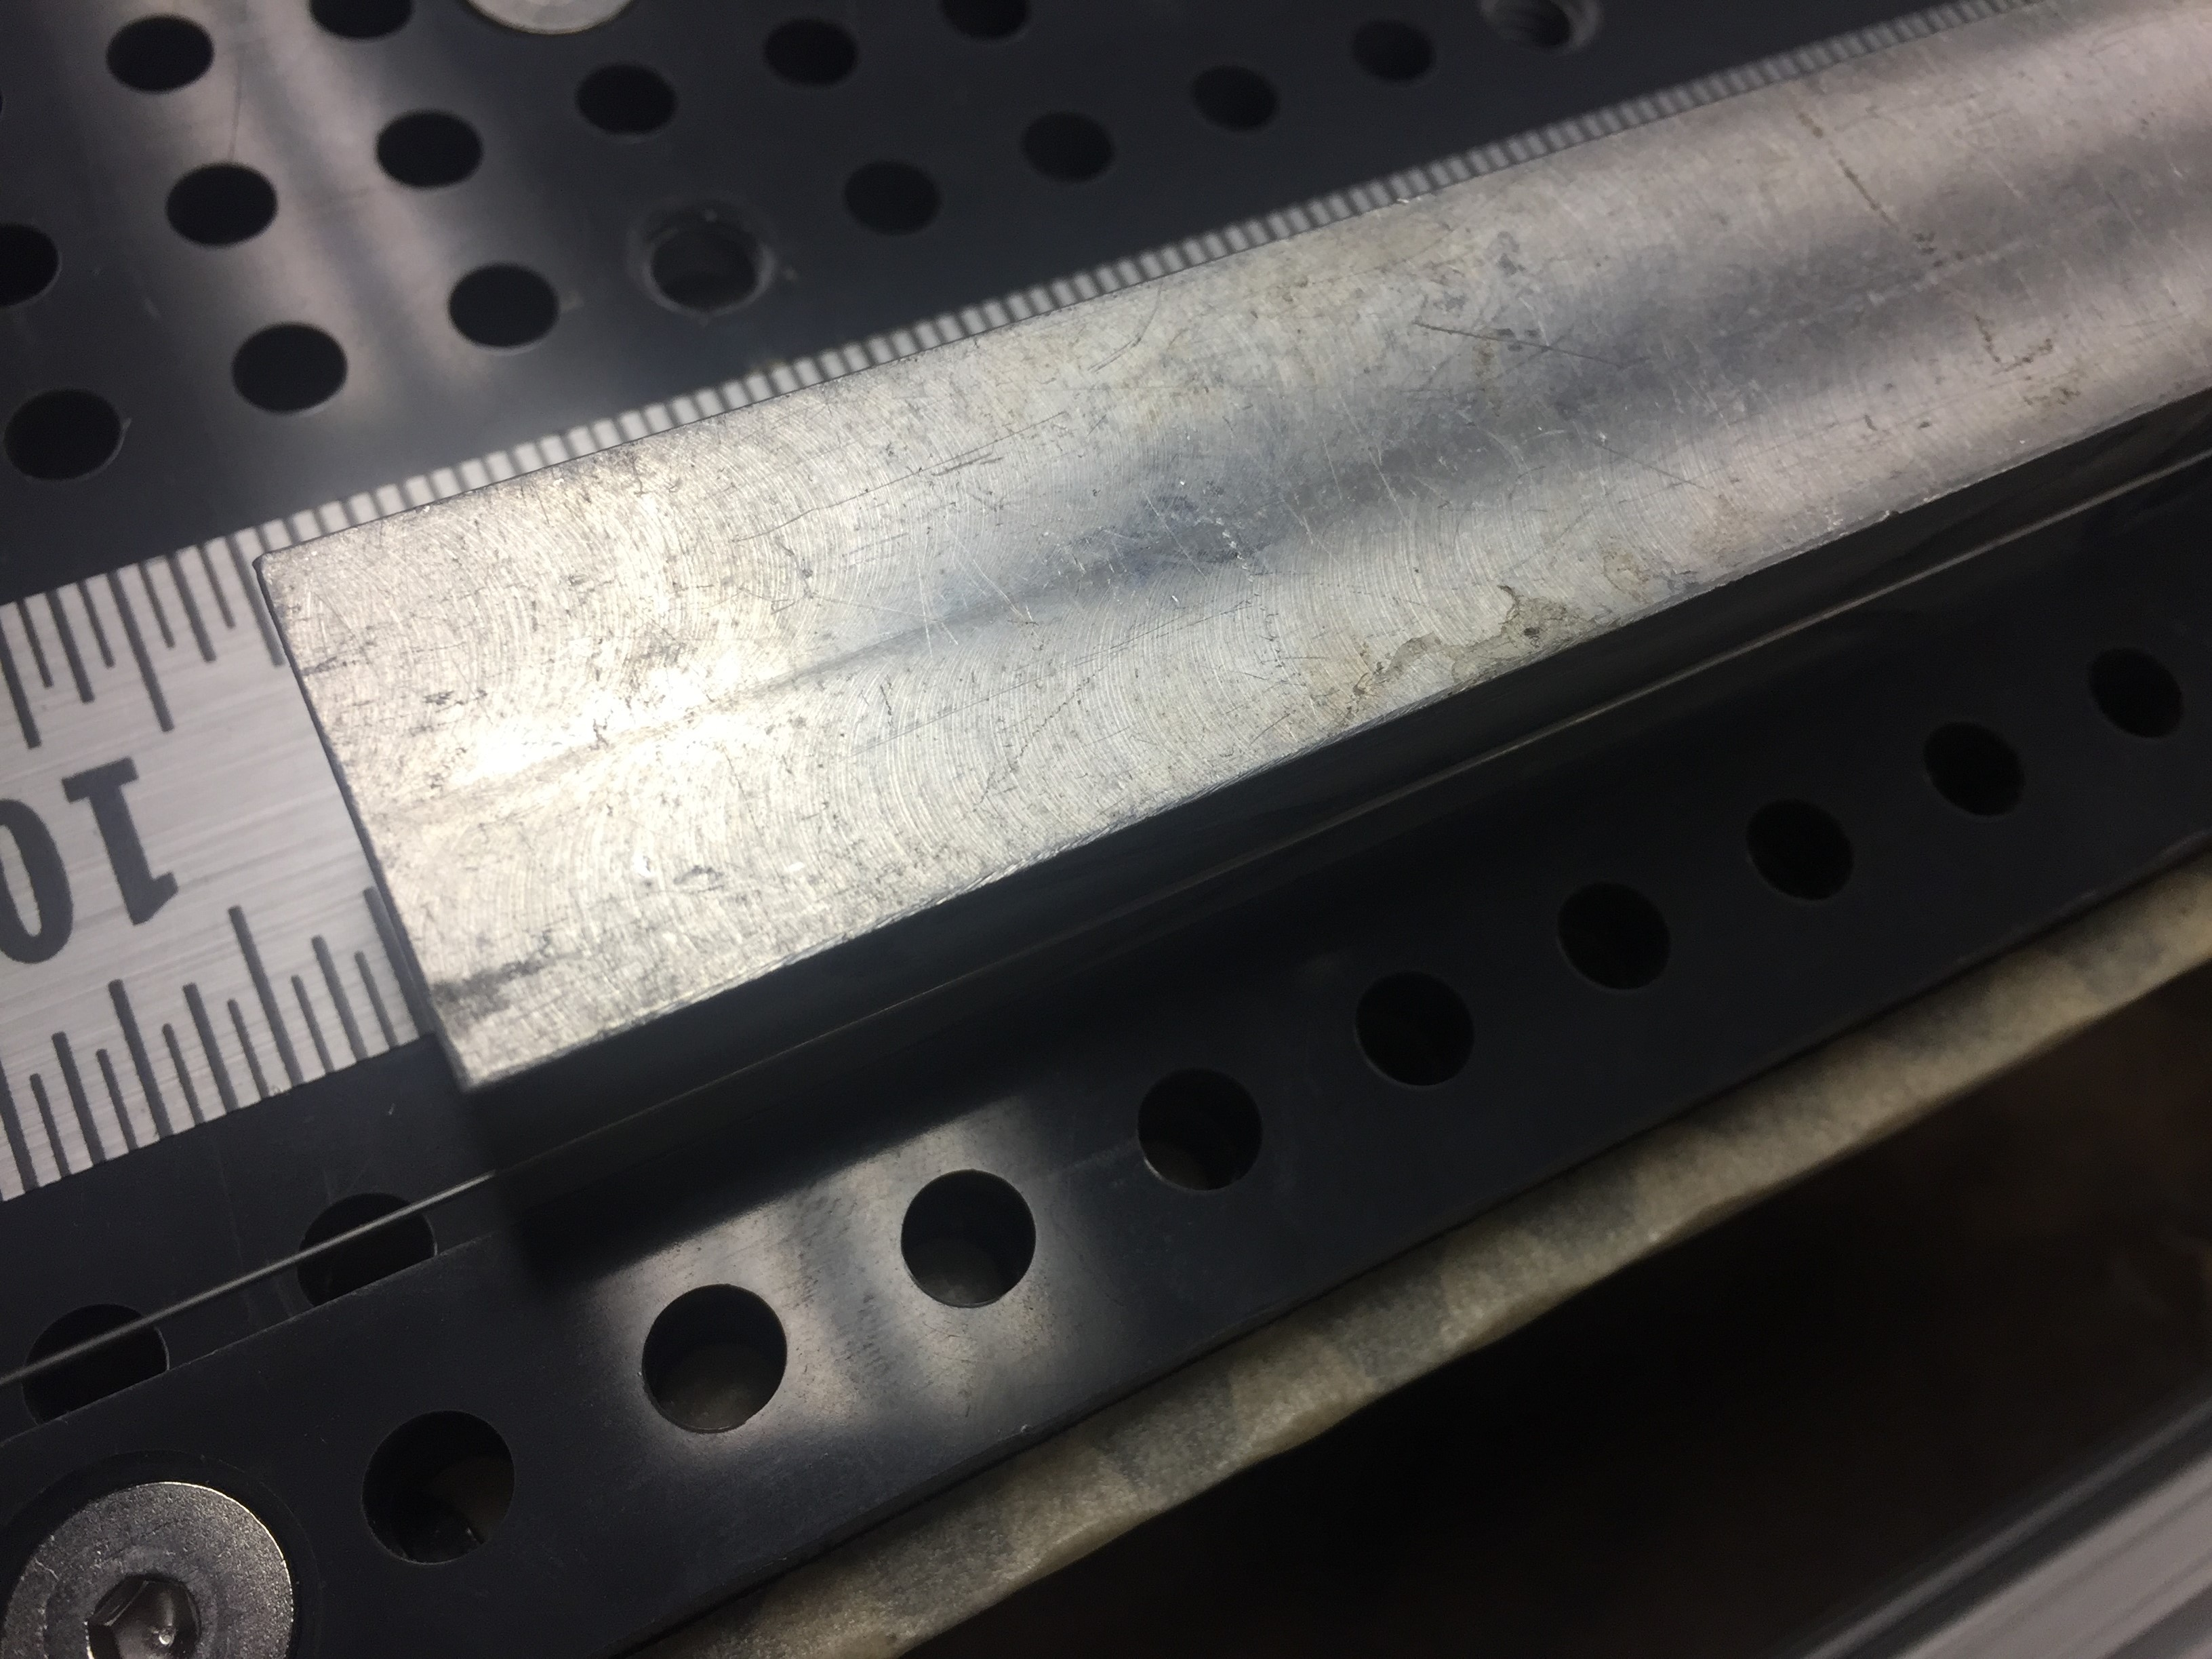
\includegraphics[width = 0.8\linewidth]{./Figures/zero_wire_1.jpg}
	\caption{Calibrate Wire Origin in the Horizontal Direction}
	\label{fig:zero1}
\end{figure}
\item Again, place a Aluminum block on the work panel against the work panel guiding block, but observe horizontally as shown in fig~\ref{fig:zero2} below. Both the far left and the far right of the wire should sit at the same height. The height could be arbitrary, but should be higher than the thumb screws on the work panel. Again, measure the amount that needs to be adjusted in millimeters.
\begin{figure} [H]
	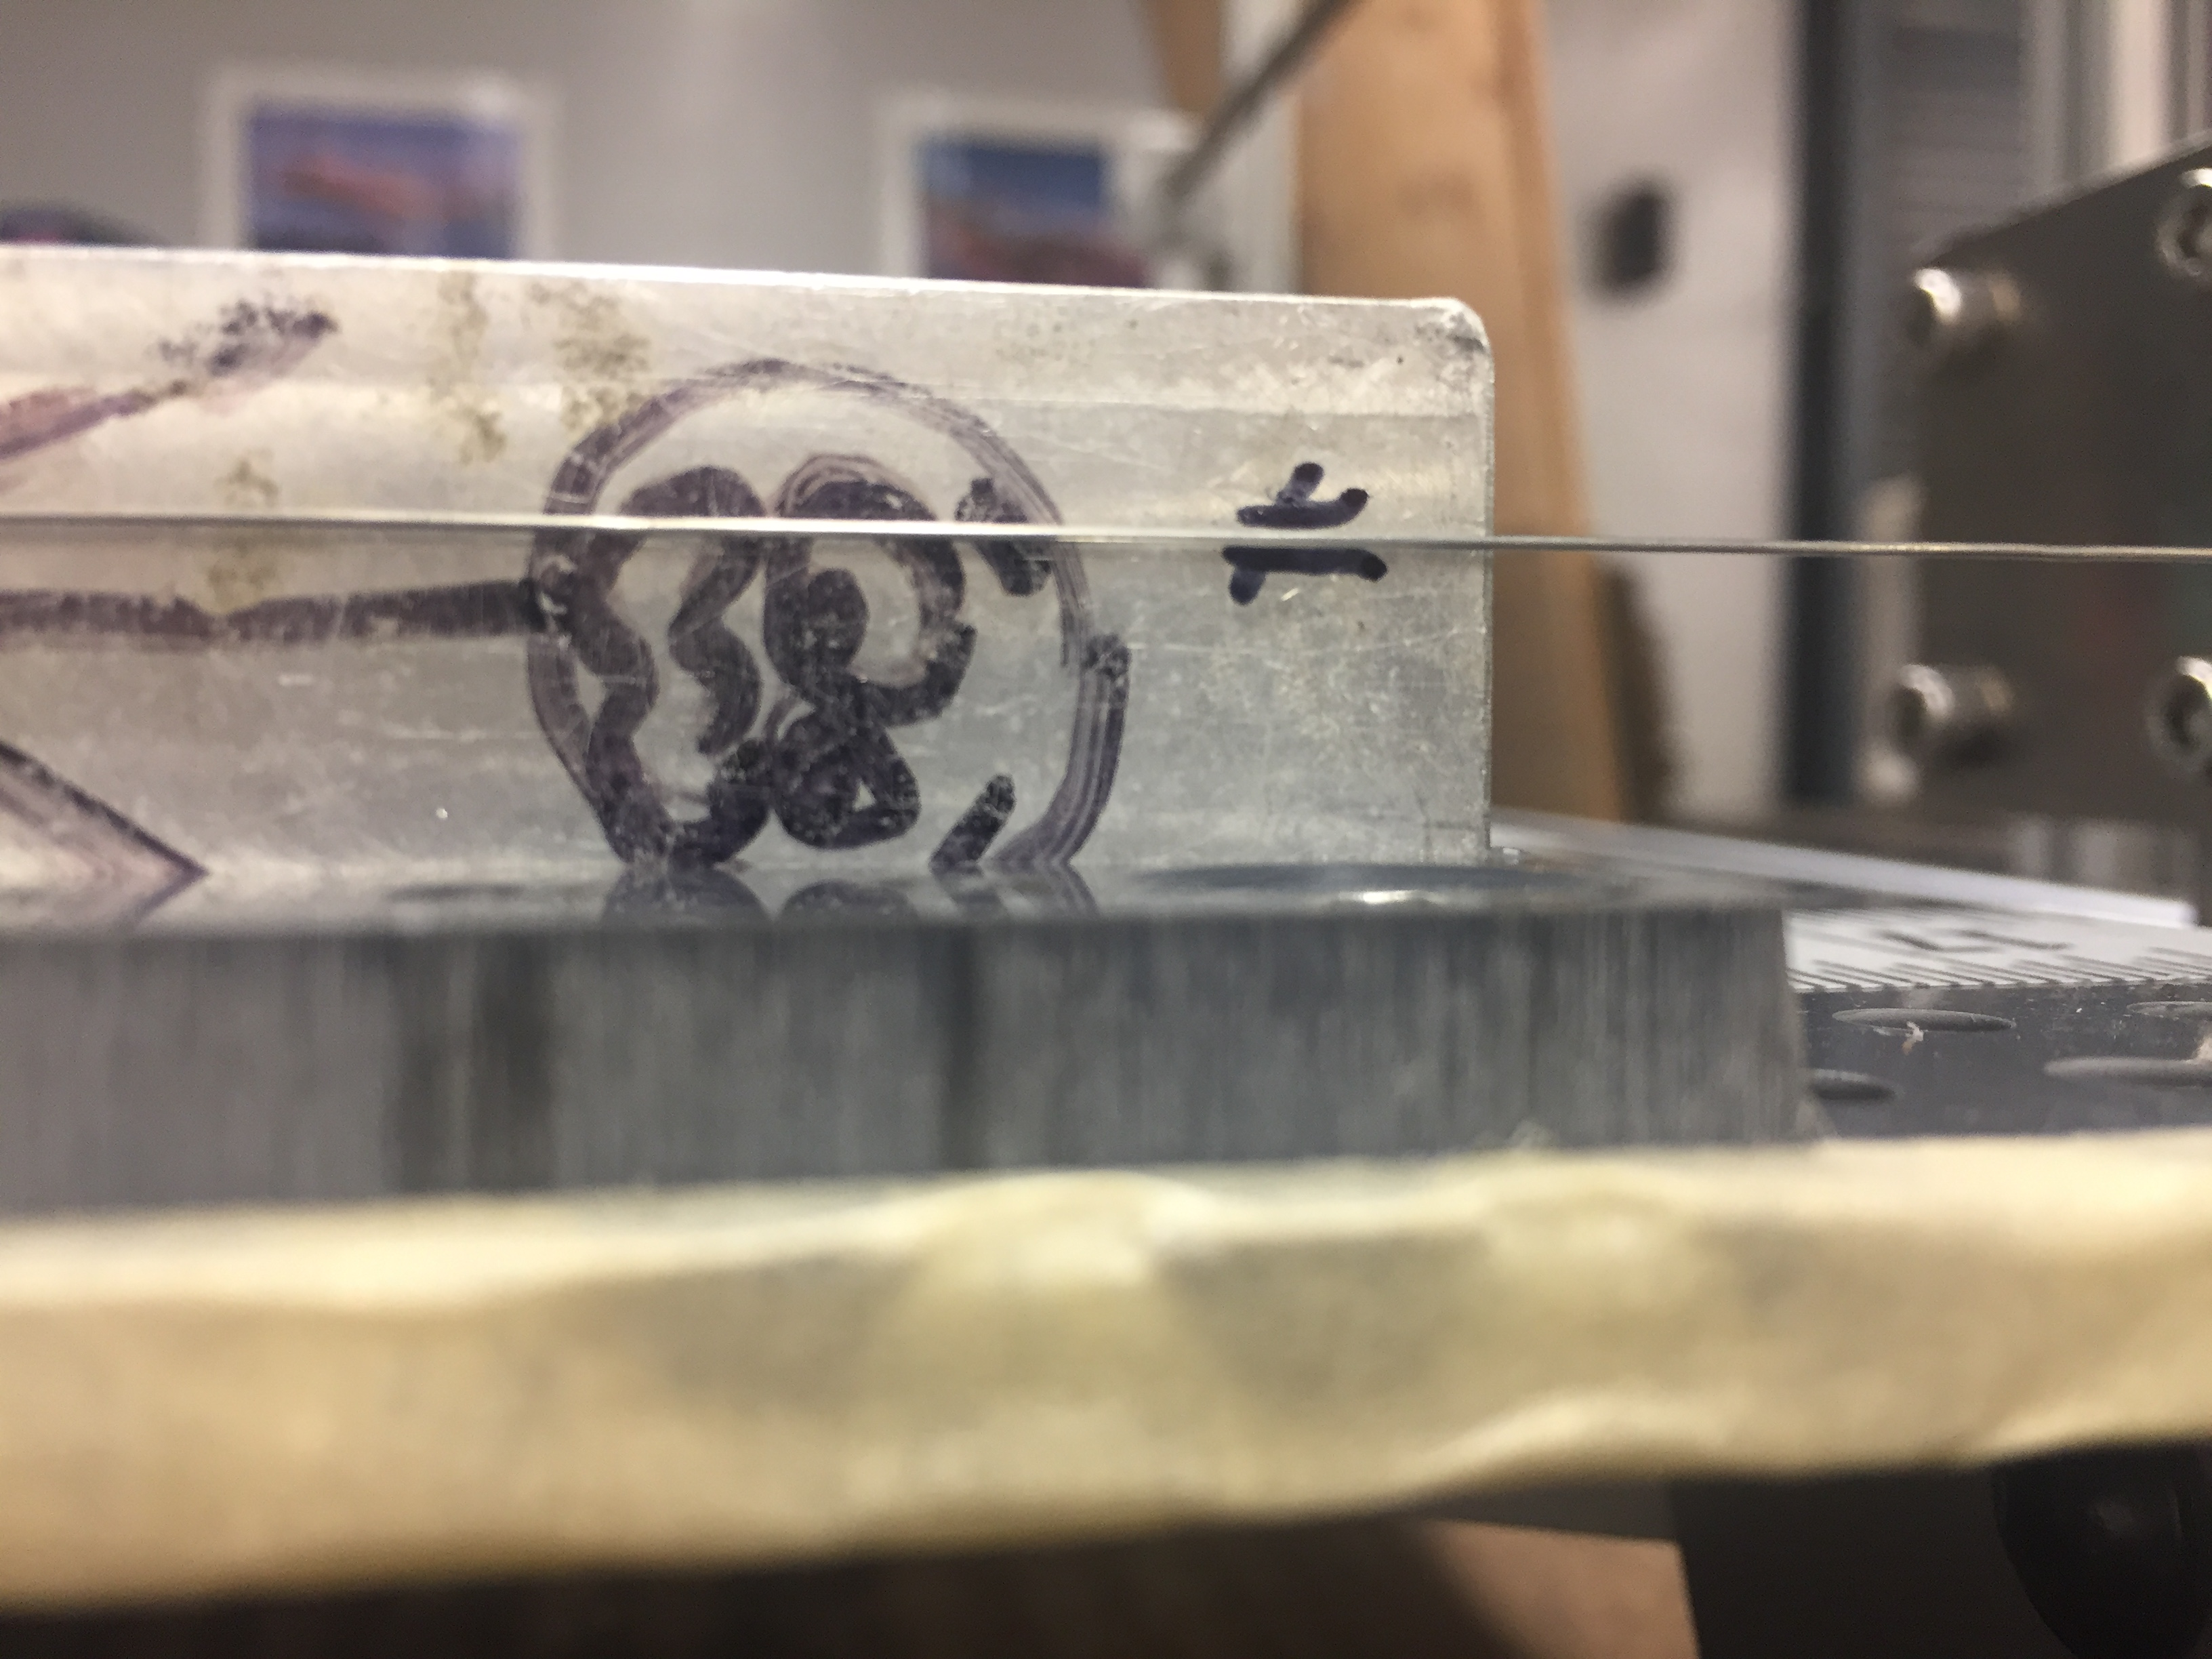
\includegraphics[width = 0.8\linewidth]{./Figures/zero_wire_2.jpg}
	\caption{Calibrate Wire Origin in the Vertical Direction}
	\label{fig:zero2}
\end{figure}
\item In WinSCP, navigate to \textbf{``/home/pi/foamcutter''} on the Pi (the right hand side of the WinSCP window), and double click on the file \textbf{``foamcutter\_setup.h''} to edit it. 
\item Find the 5 lines that read as the following:\\ \\
\textbf{// position of limit switch relative to cutter origin}\\
\textbf{\#define LIM2ORIGIN\_LX -4100}\\
\textbf{\#define LIM2ORIGIN\_RX -3550}\\
\textbf{\#define LIM2ORIGIN\_LY -2500}\\
\textbf{\#define LIM2ORIGIN\_RY -2400}\\ \\
and adjust the four numbers: if wish to move an axis 1mm further away (or closer) from the limit switch, subtract (or add) 157 from the number corresponding to the axis. \textbf{All 4 numbers must be negative integers, no decimal, and no equations (please calculated the number yourself and replace the original number).}
\item Save the file then repeat the process from step 4 to adjust the 4 numbers until the wire sits at the desired location. \textbf{Then save the 4 numbers on your computer.}
\item In PuTTY, run the following commands line by line:
\begin{itemize}[noitemsep,topsep=0pt]
	\item \textbf{cd}
	\item \textbf{cd foamcutter}
	\item \textbf{sudo make install foamcutter}
\end{itemize}
\item In WinSCP, delete the folder \textbf{``/home/pi/foamcutter''} on the Pi.
\item You can now use \textbf{sudo foamcutter} in PuTTY to run the foamcutter program.
\end{enumerate}

\subsection{Install/Update the Foamcutter Software Without Wire Calibration}
\label{sec:install}
\begin{enumerate}[itemsep = 5pt,topsep=0pt]
\item Download the \textbf{``User Package.zip''} from \href{https://github.com/ythuang96/FoamCutter}{https://github.com/ythuang96/FoamCutter}, and unzip it.
\item In WinSCP, create a new folder on the Pi called \textbf{``foamcutter''} in the directory of \textbf{``/home/pi''}. 
\item In WinSCP, upload the files named \textbf{``foamcutter.c''}, \textbf{``foamcutter\_setup.h''} and \textbf{``Makefile''} from the \textbf{''User Package''} just downloaded into the \textbf{``foamcutter''} folder just created on the Pi.
\item In WinSCP, edit the file \textbf{``/home/pi/foamcutter\_setup.h''}, find the 5 lines that read as the following:\\ \\
\textbf{// position of limit switch relative to cutter origin}\\
\textbf{\#define LIM2ORIGIN\_LX -4100}\\
\textbf{\#define LIM2ORIGIN\_RX -3550}\\
\textbf{\#define LIM2ORIGIN\_LY -2500}\\
\textbf{\#define LIM2ORIGIN\_RY -2400}\\ \\
and change the 4 numbers to the previously calibrated parameters. (If you do not have previous calibration parameters, it is recommended to follow Section~\ref{sec:calibration} to install and calibrate the origin.)
\item In PuTTY, run the following commands line by line:
\begin{itemize}[noitemsep,topsep=0pt]
	\item \textbf{cd}
	\item \textbf{cd foamcutter}
	\item \textbf{sudo make install foamcutter}
\end{itemize}
\item In WinSCP, delete the folder \textbf{``/home/pi/foamcutter''} on the Pi.
\item You can now use \textbf{sudo foamcutter} in PuTTY to run the foamcutter program.
\end{enumerate}

\section{G-Code Generation}
\label{sec:gcode}
\subsection{G-Code for Wing}
\begin{enumerate}[itemsep = 5pt,topsep=0pt] 
	\item Download the needed airfoil coordinates at \\ \href{http://m-selig.ae.illinois.edu/ads/coord_database.html#S}{http://m-selig.ae.illinois.edu/ads/coord\_database.html\#S}
	\item Place the needed airfoil coordinate files in the same folder as the MatLab code \\ \textbf{``DBF\_foamcutter\_wing.m''} which is provided in the \textbf{``User Package.zip''} from \\ \href{https://github.com/ythuang96/FoamCutter}{https://github.com/ythuang96/FoamCutter}.
	\item Enter the parameters into the MatLab script and run the script. A figure tracing the the motion of the two ends of the wire should show up, and the G-code should be saved in the same folder.
\end{enumerate}

\noindent Note:

When cutting extremely tampered parts, figure similar to the fig~\ref{fig:wing1} below might show up during the G-code generation process:
\begin{figure} [H]
	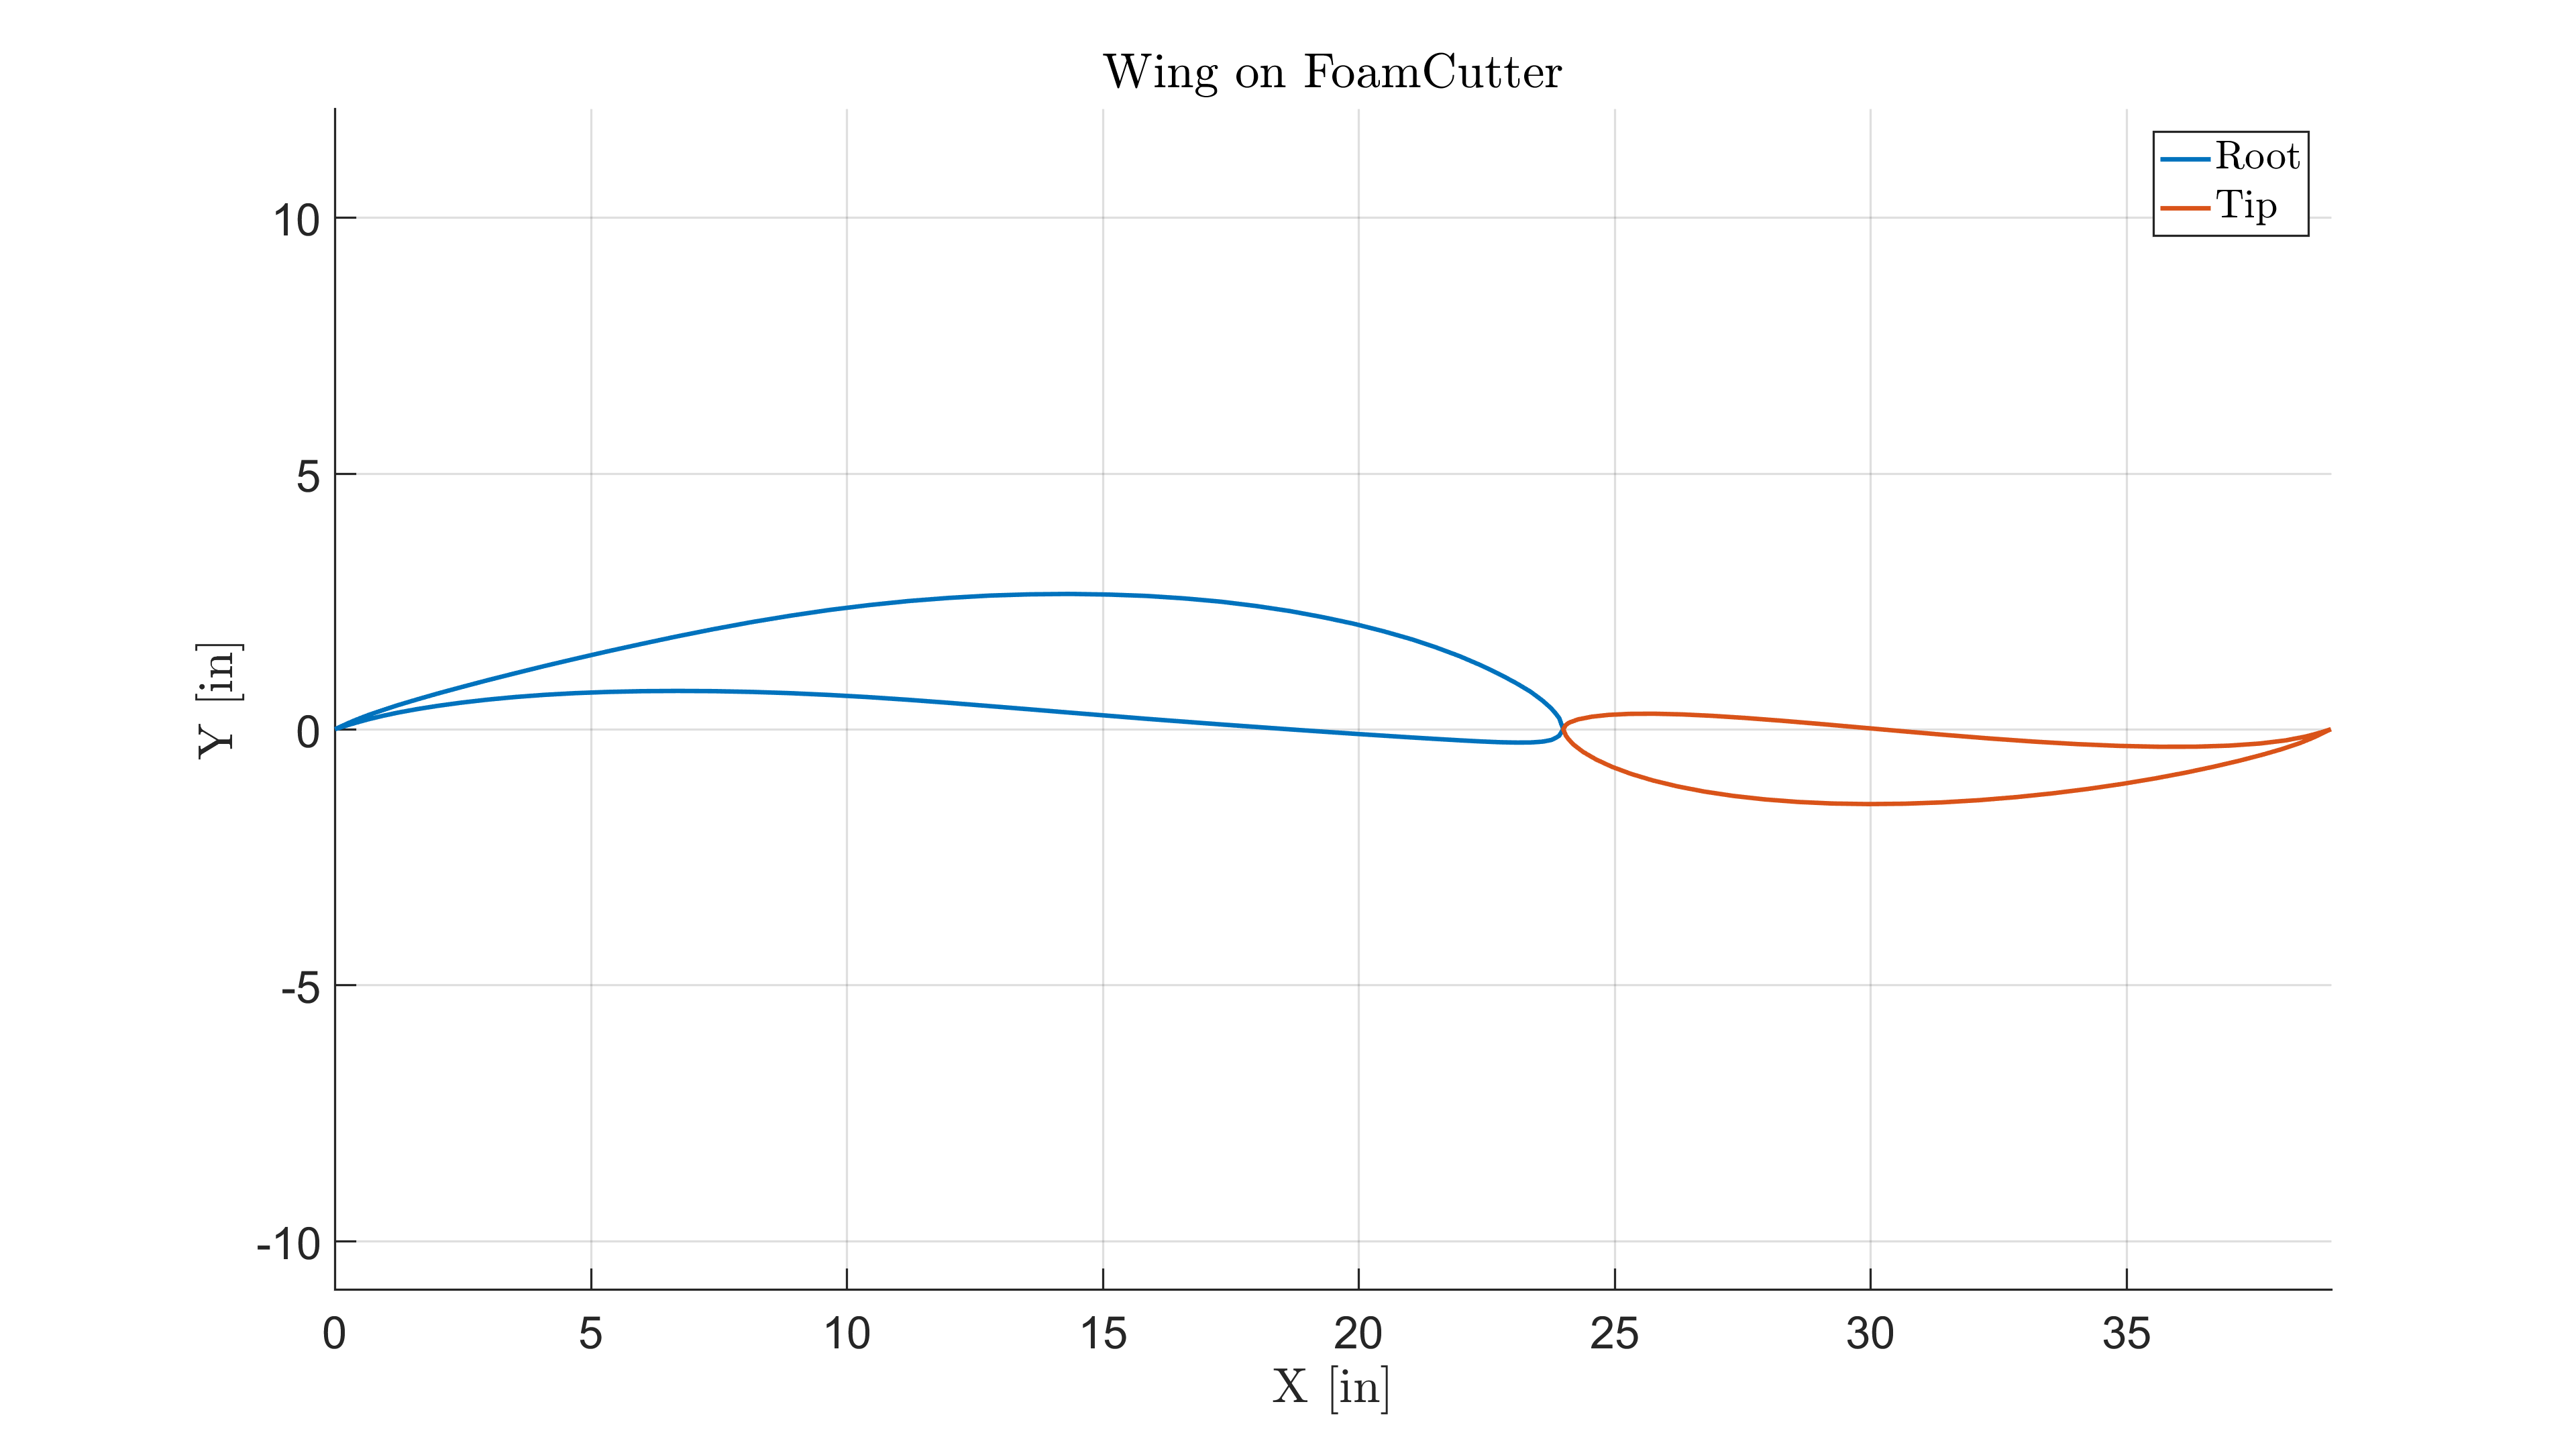
\includegraphics[width = 0.9\linewidth]{./Figures/wing_example.png}
	\caption{Example Figure During G-code Generation for a Wing}
	\label{fig:wing1}
\end{figure}
The parameters used for this figure is shown below:
\begin{figure} [H]
	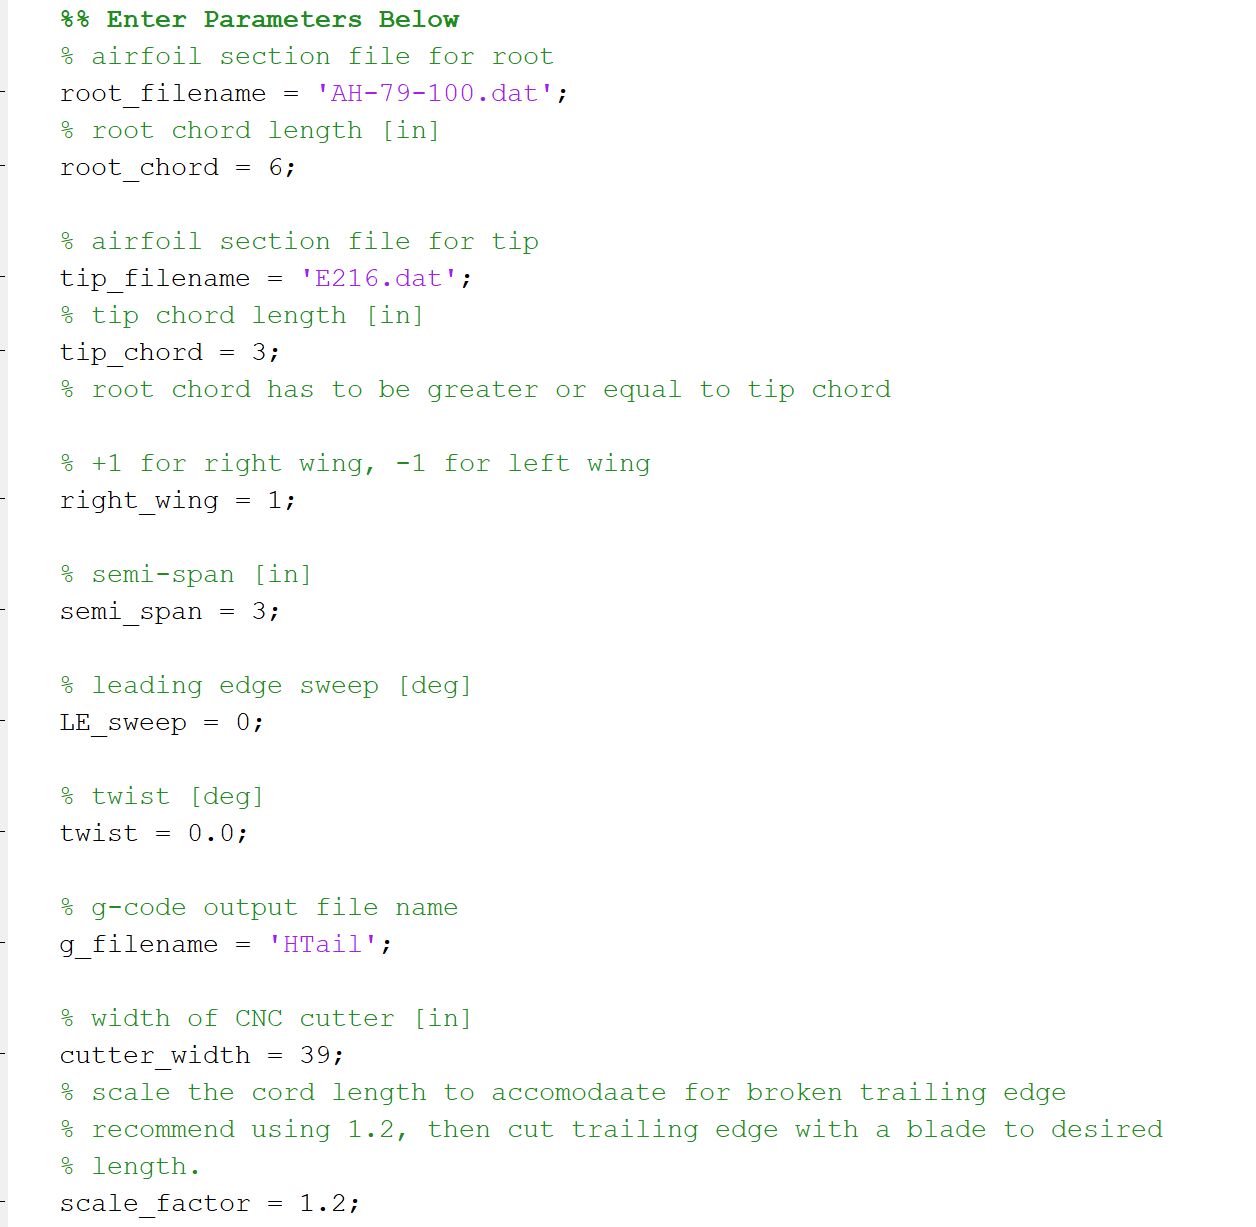
\includegraphics[width = 0.7\linewidth]{./Figures/wing_example2.png}
	\caption{Example Parameters During G-code Generation for a Wing}
	\label{fig:wing2}
\end{figure}
Note that the root and tip cord length differed a lot, and the span is significantly smaller than the cutter width, therefore, this is an extremely tapered cut. As a result, the inverted airfoil shown in fig~\ref{fig:wing1} above is expected. As explained in fig~\ref{fig:wing3} below, for extremely tapered cuts, the two ends of the wire could move in opposite directions, resulting in the inverted airfoil shown in fig~\ref{fig:wing1}.
\begin{figure} [H]
	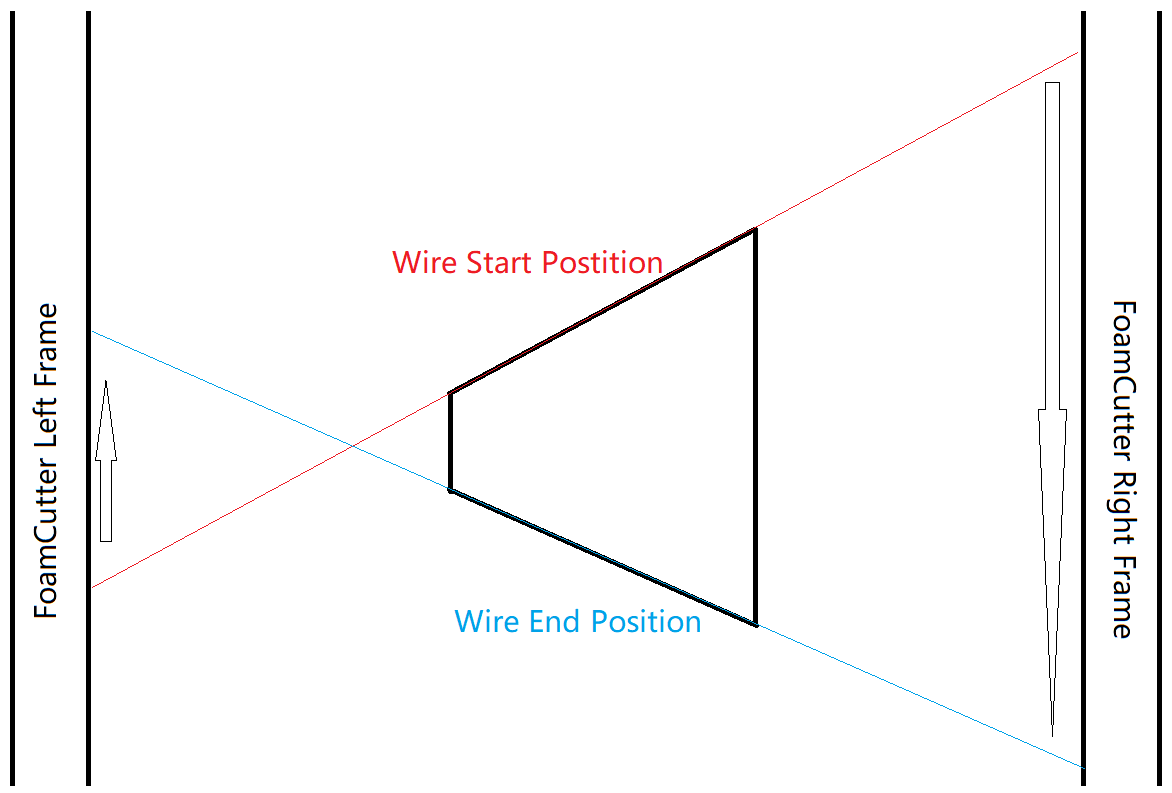
\includegraphics[width = 0.55\linewidth]{./Figures/wing_example3.png}
	\caption{Sketch of an Extremely Tapered Cut}
	\label{fig:wing3}
\end{figure}

\subsection{G-Code for General Shapes}
\begin{tcolorbox}
	{\large
		\noindent Key Points:
		\begin{itemize}[noitemsep,topsep=0pt]
			\item Make sure to increase AutoCAD precision;
			\item Make sure to scale the drawing by 25.4 in AutoCAD if the SolidWorks file is in inches;
			\item Make sure to run ``Explode'' command in AutoCAD;
			\item Make sure there are no overlapping lines;
			\item Make sure to convert spline to polyline in AutoCAD and explode again.
		\end{itemize}
	}
\end{tcolorbox}

\begin{enumerate}[itemsep = 5pt,topsep=0pt]
	\item Export the projection of the top or side (or both) profiles from SolidWorks into .dxf files, the steps are demonstrated with the payload bay shown in fig~\ref{fig:sw1} below.
	\begin{figure} [H]
		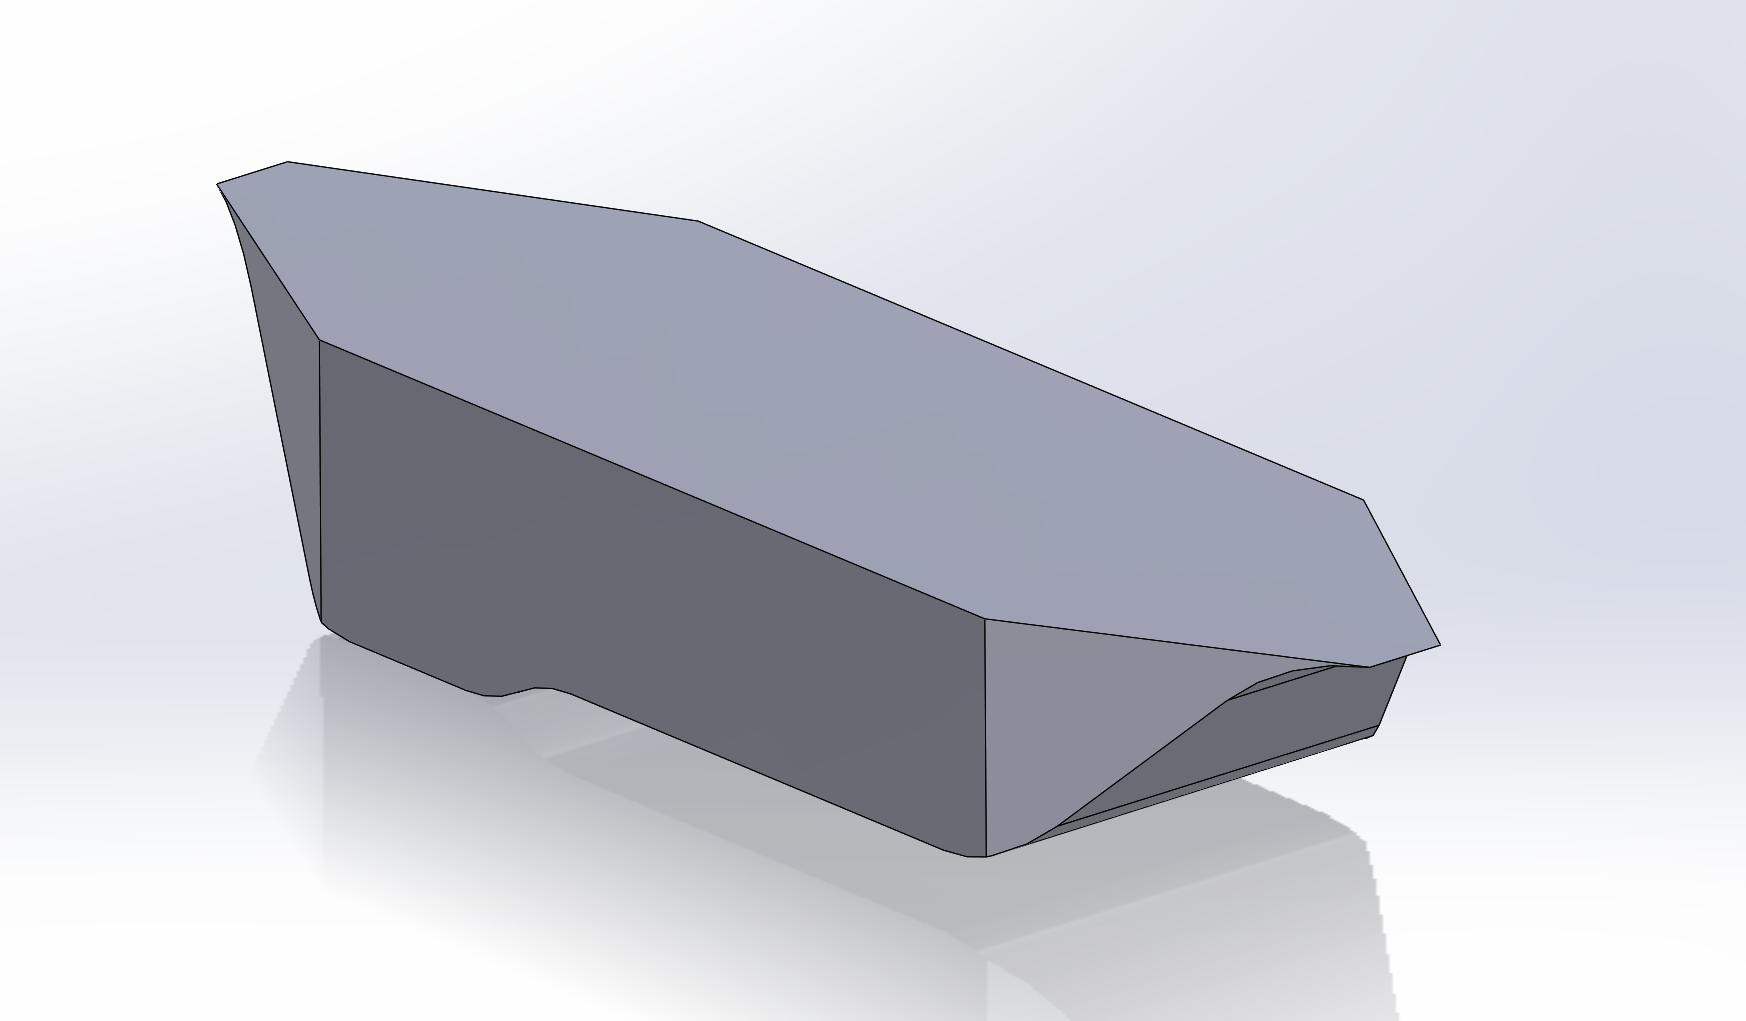
\includegraphics[width = 0.6\linewidth]{./Figures/general_shape/sw1.png}
		\caption{Sample Payload Bay}
		\label{fig:sw1}
	\end{figure}
	\begin{itemize}[noitemsep,topsep=0pt]
		\item The projection of the side profile can be obtained by slicing the part vertically in the center: go to ``Insert $\rightarrow$ Features $\rightarrow$ Split'' as shown in fig~\ref{fig:sw2} below:
		\begin{figure} [H]
			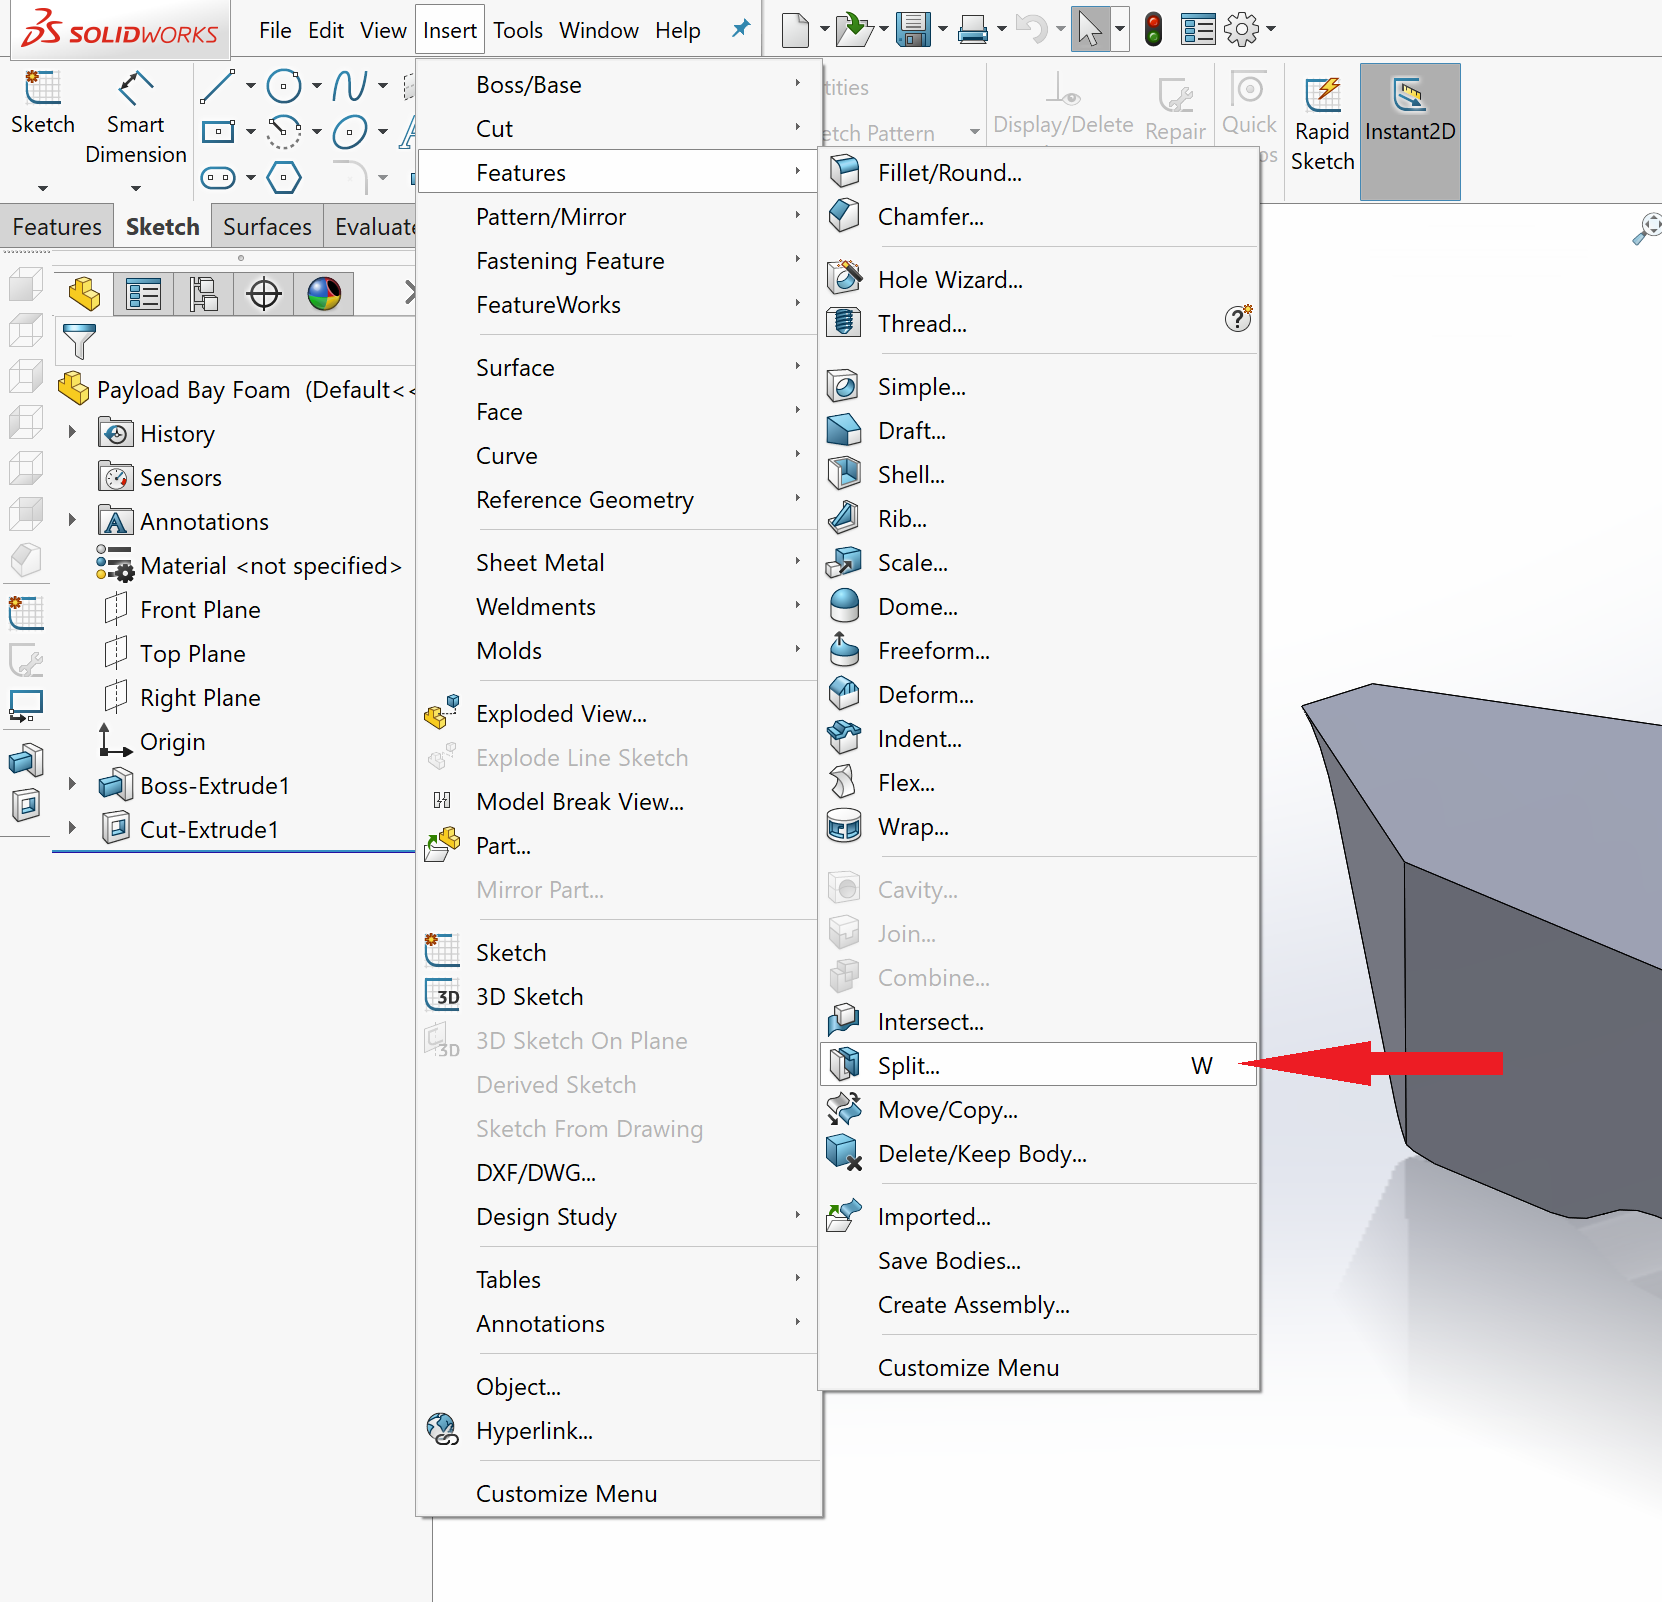
\includegraphics[width = 0.6\linewidth]{./Figures/general_shape/sw2.png}
			\caption{SolidWorks Split Command}
			\label{fig:sw2}
		\end{figure}
		
		\item In the pop up window, as shown in fig~\ref{fig:sw3} below, in ``Trim Tools'' selected the desired plane (the front plane in this case) then click ``Cut Body''. In the ``Resulting Bodies'' box, select one of the resulting bodies. Lastly, make sure the ``Consume cut bodies'' check box is selected, and click the top left green check mark. This will delete the selected half of the part (the brown half in fig~\ref{fig:sw3}).
		\begin{figure} [H]
			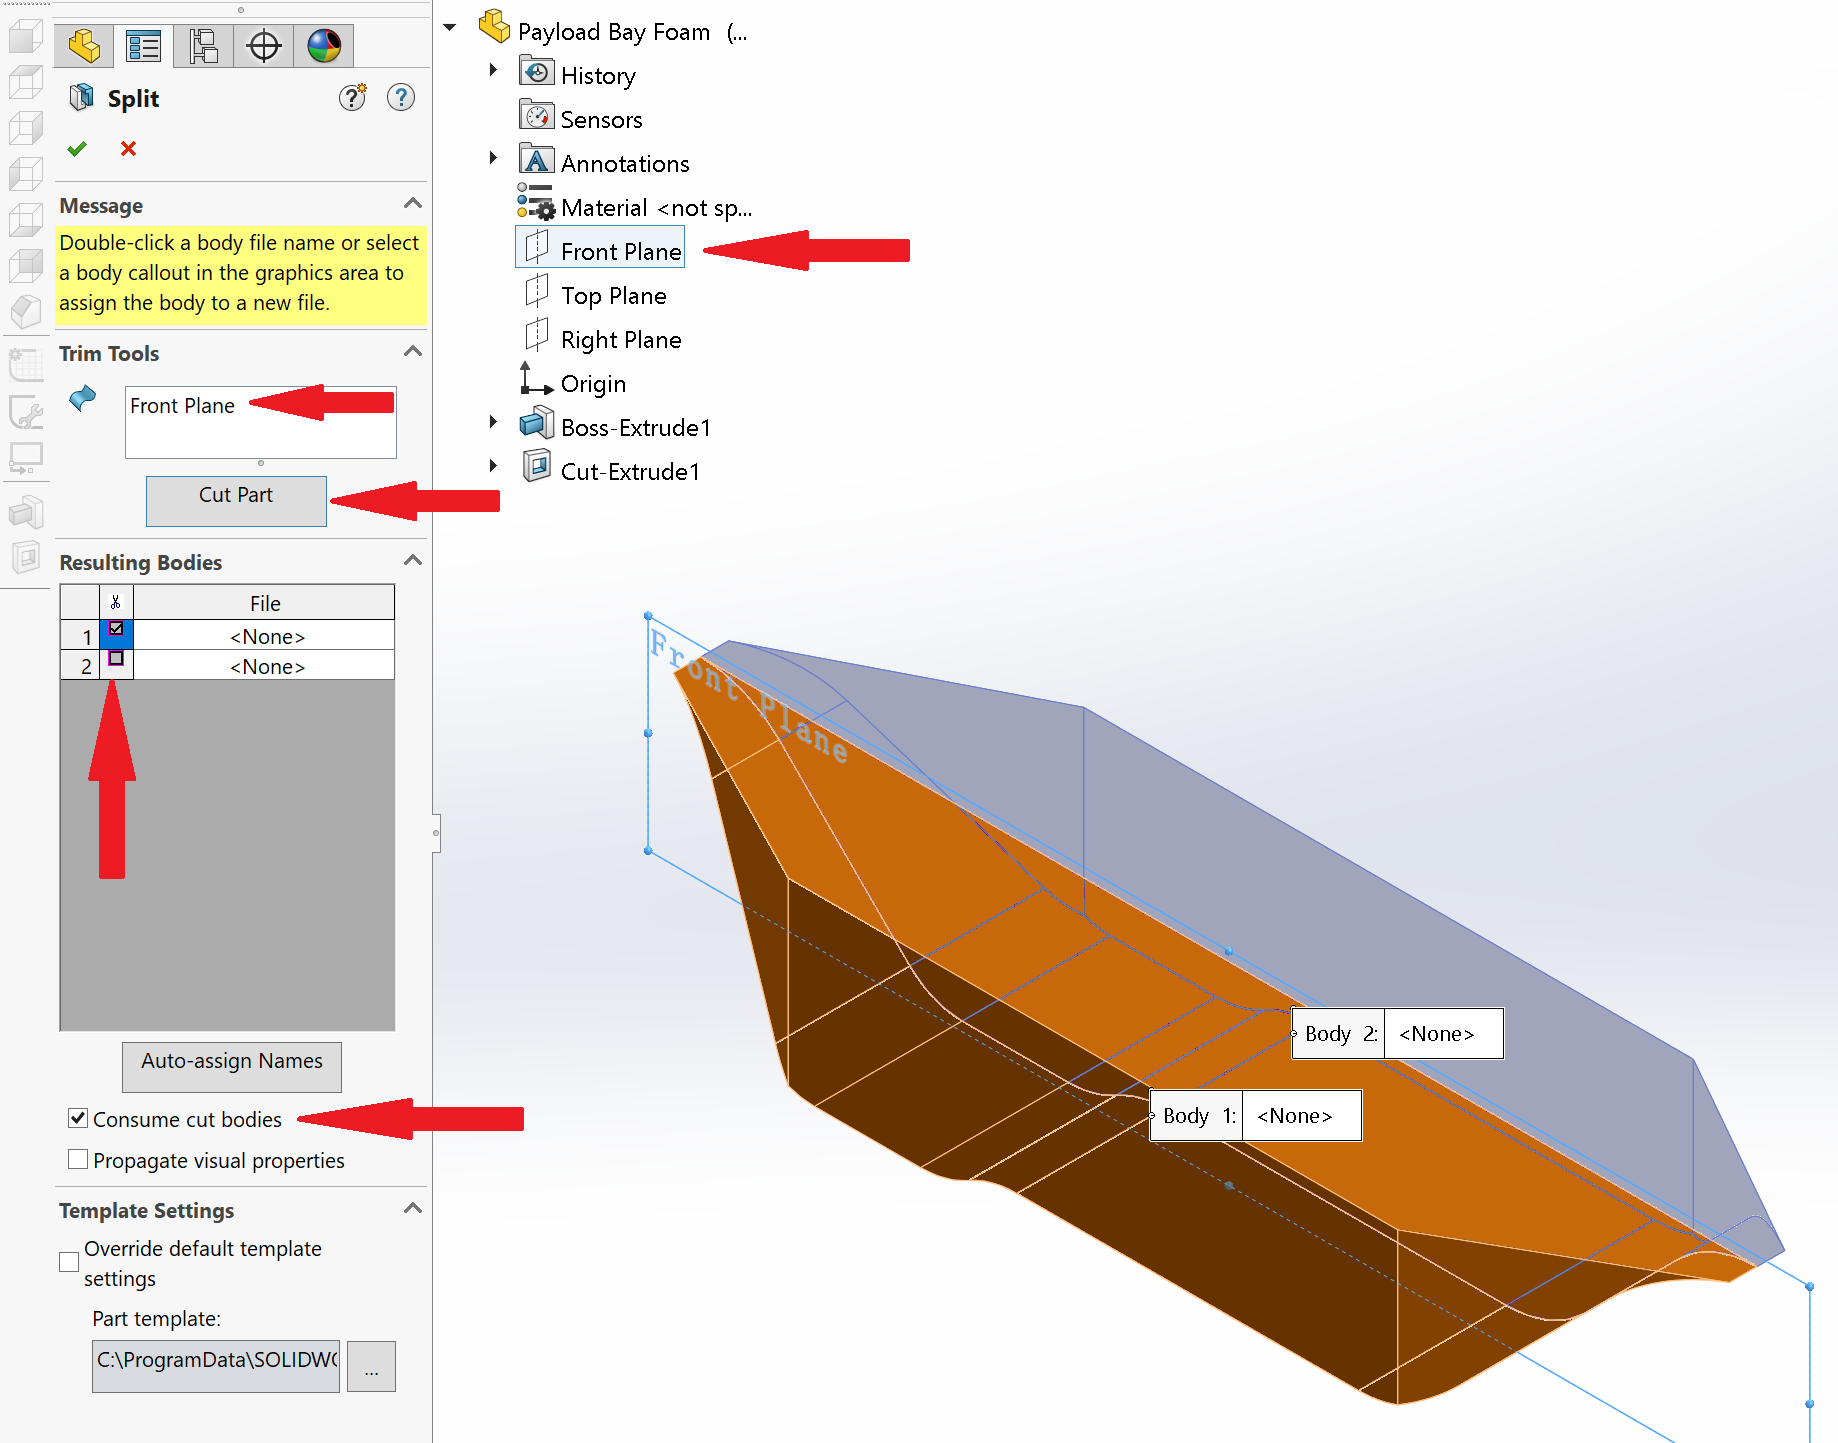
\includegraphics[width = 0.9 \linewidth]{./Figures/general_shape/sw3.png}
			\caption{SolidWorks Split Menu}
			\label{fig:sw3}
		\end{figure}
		
		\item Right click on the cut plane and select ``Export to DXF/DEG'' to export the projection of the side profile as shown in fig~\ref{fig:sw4} below:
		\begin{figure} [H]
			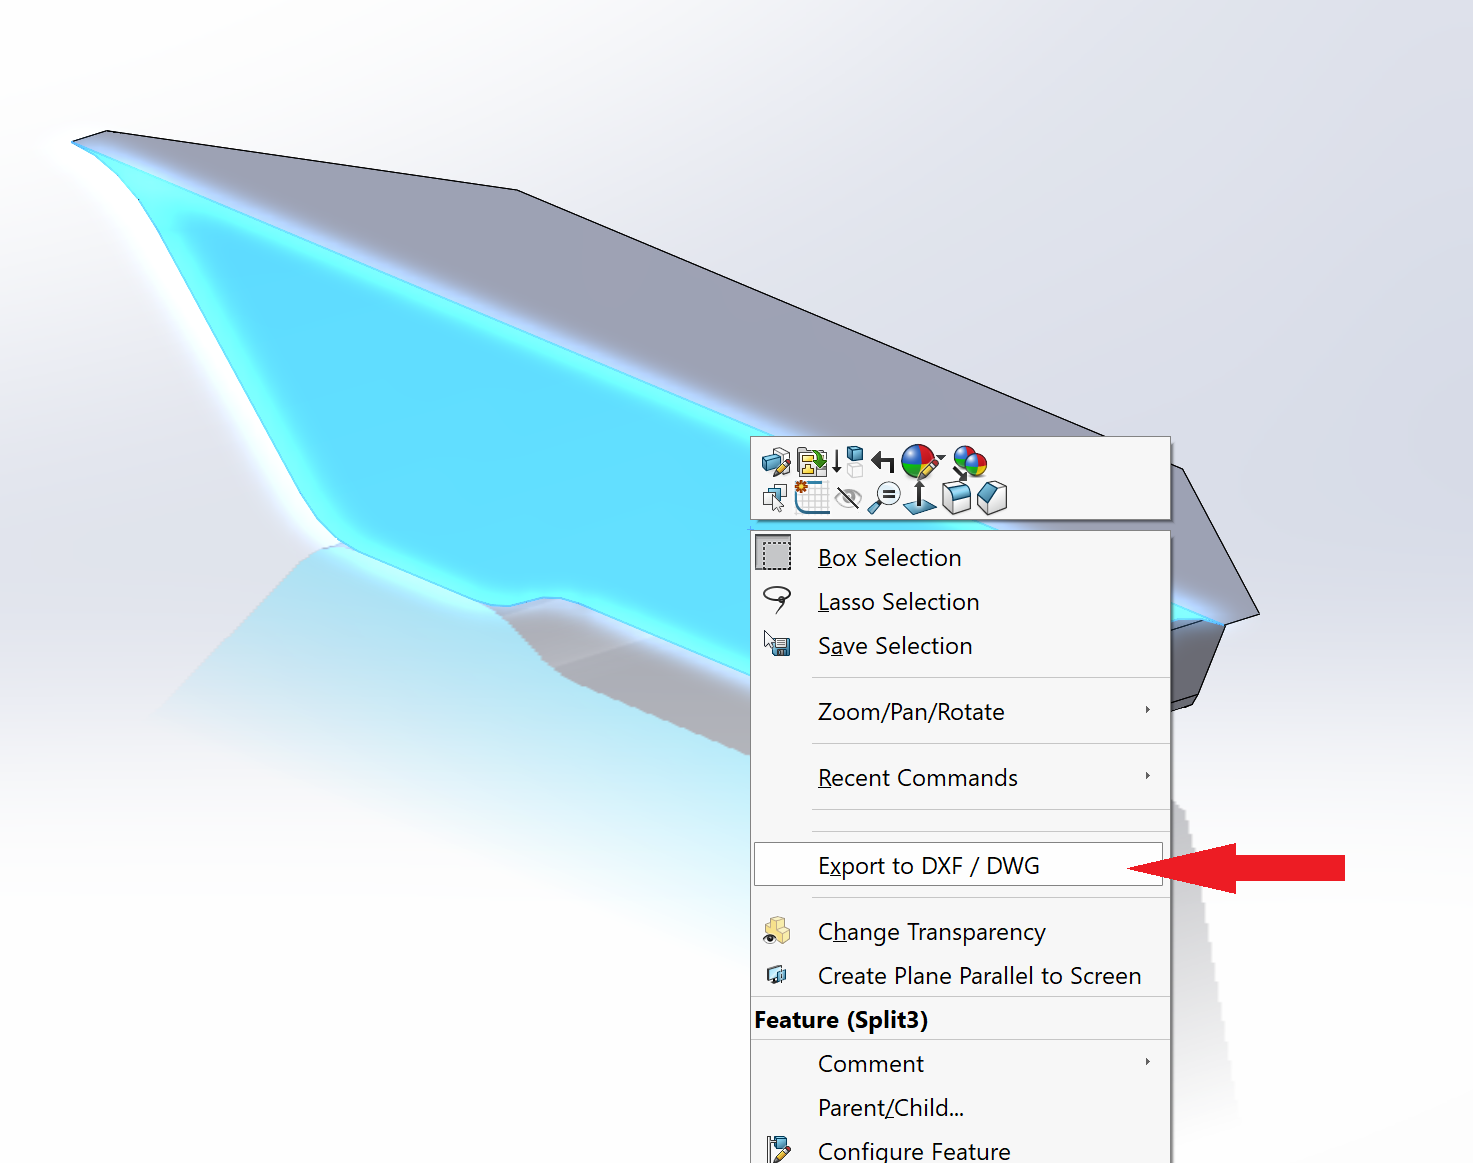
\includegraphics[width = 0.6\linewidth]{./Figures/general_shape/sw4.png}
			\caption{Export Side Profile}
			\label{fig:sw4}
		\end{figure}
		
		\item The top plane of the part is the projection from above, therefore, skip the split command and directly right click on the plane and export:
		\begin{figure} [H]
			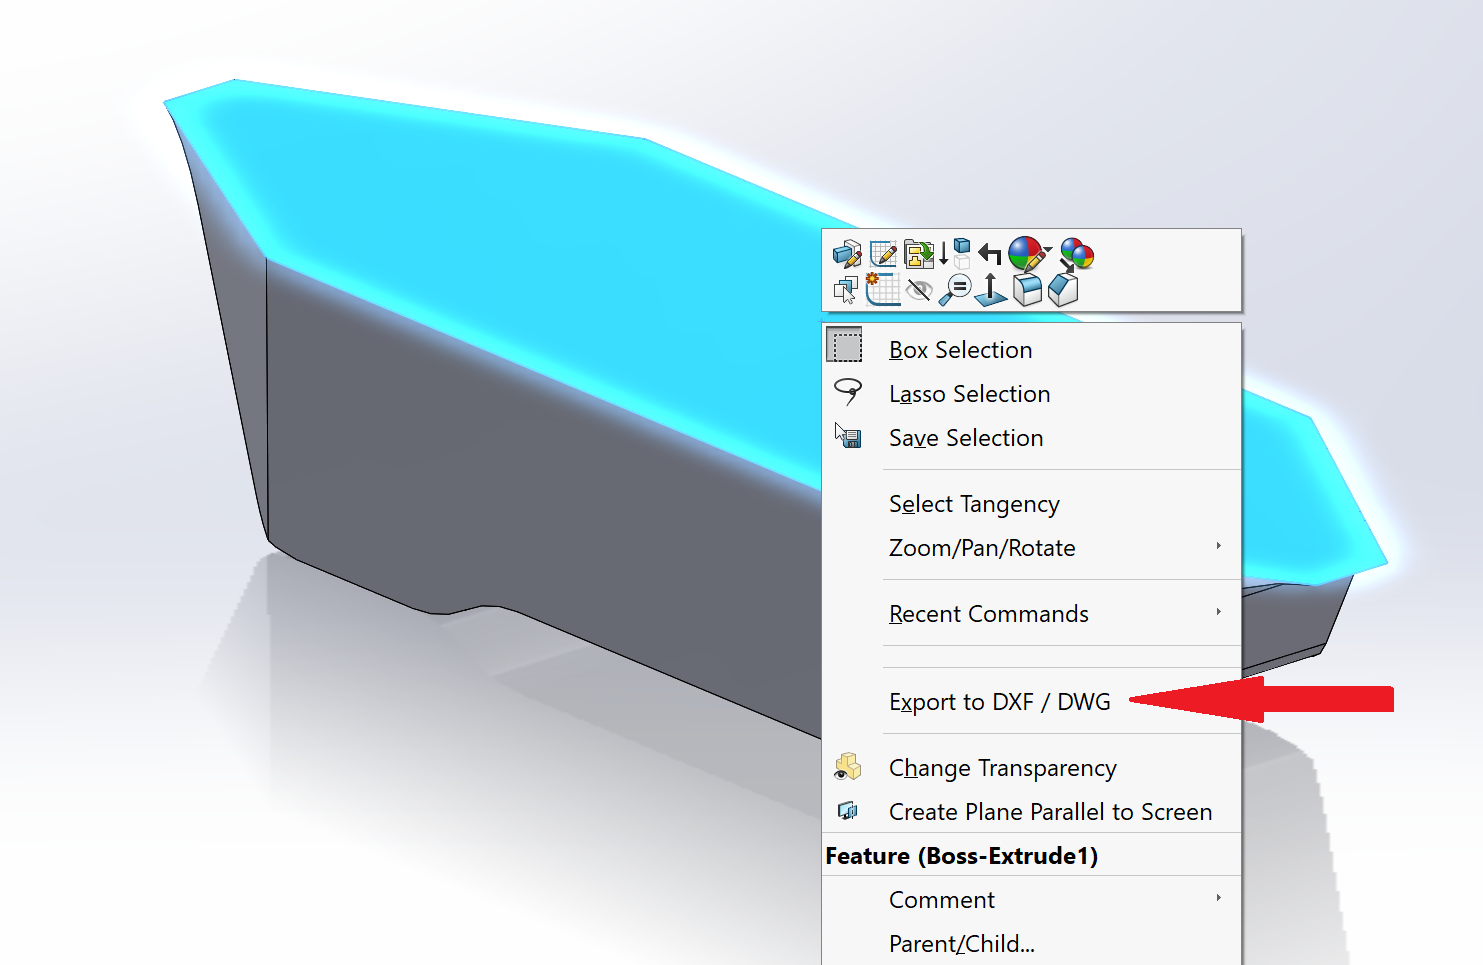
\includegraphics[width = 0.6\linewidth]{./Figures/general_shape/sw5.png}
			\caption{Export Top Profile}
			\label{fig:sw5}
		\end{figure}
		
	\end{itemize}
	
	\item Open AutoCAD, increase the precision by clicking the top left red AutoCAD sign, select ``Drawing Utilities $\rightarrow$ Units'' and increase the precision to 4 decimal points, as shown in fig~\ref{fig:cad1} below.
	\begin{figure}[H]
		\centering
		\begin{subfigure}[b]{.4\textwidth}
			\centering
			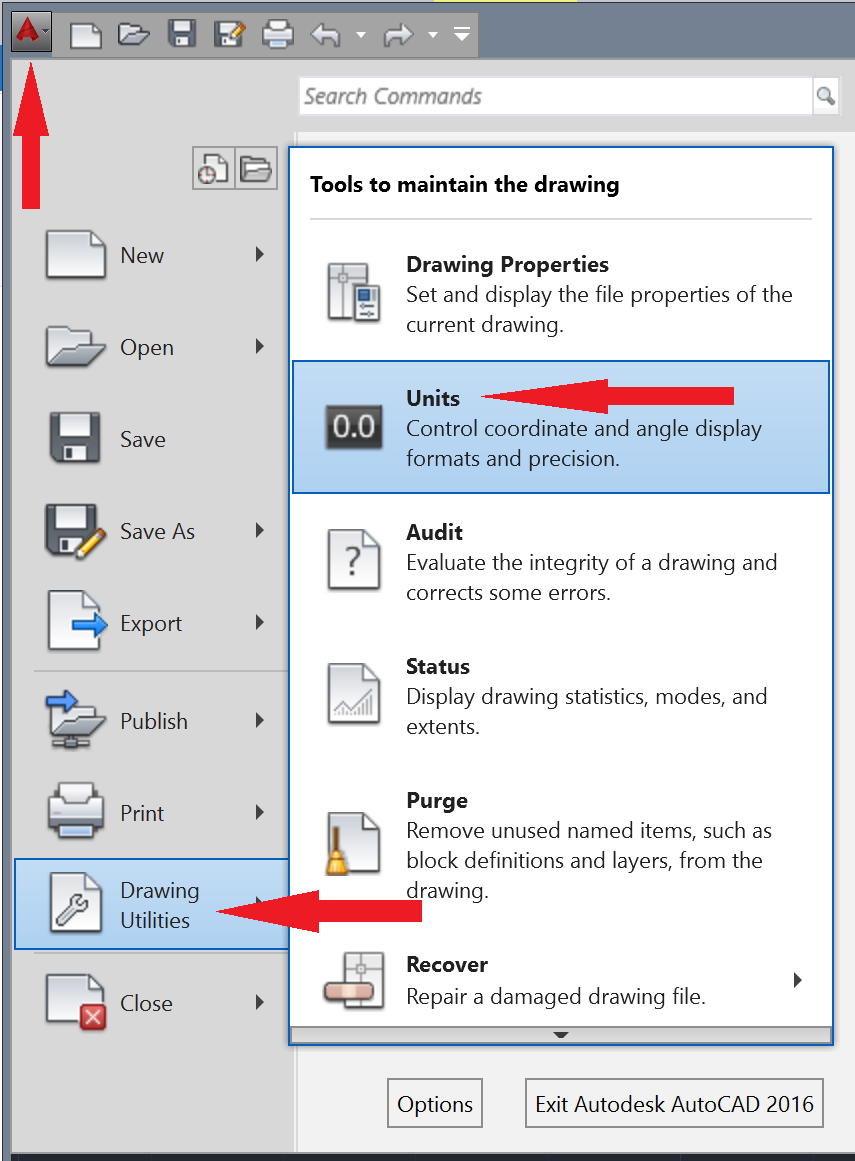
\includegraphics[width=\textwidth]{./Figures/general_shape/cad1.png}
		\end{subfigure}
		\begin{subfigure}[b]{.4\textwidth}
			\centering
			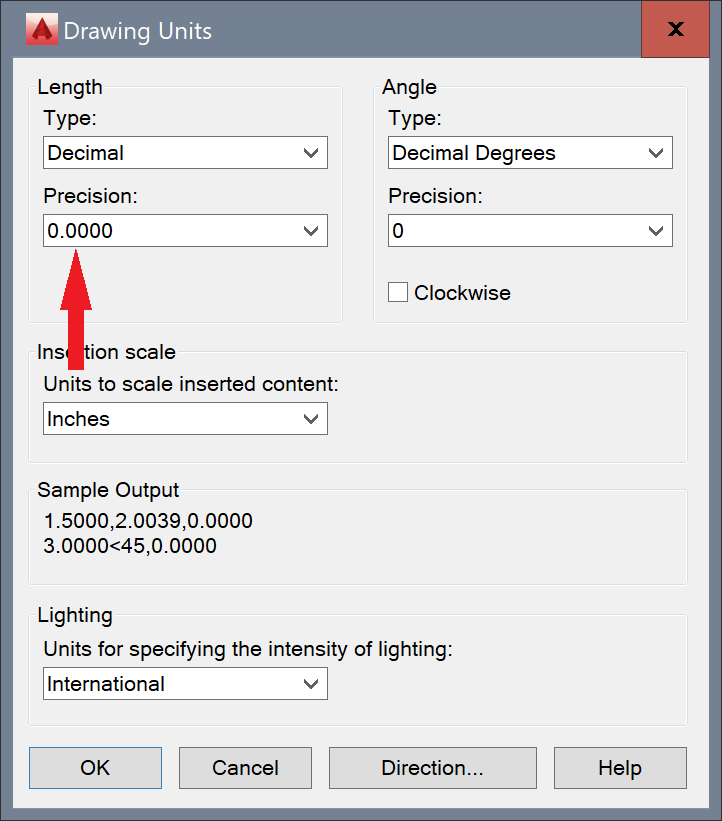
\includegraphics[width=\textwidth]{./Figures/general_shape/cad2.png}
		\end{subfigure}
		\caption{Increase AutoCAD Precision}
		\label{fig:cad1}
	\end{figure}
	
	\item Import the dxf files from SolidWorks.
	\item Scale the drawing by 25.4 if the SolidWorks file is in inches.
	\item Select all objects and run ``Explode'' command.
	\item Select all Spline (if any), right click and select ``Spline $\rightarrow$ Convert to Polyline'' as shown in fig~\ref{fig:cad3} below. When ask to enter accuracy, enter 1 and press enter.
	\begin{figure} [H]
		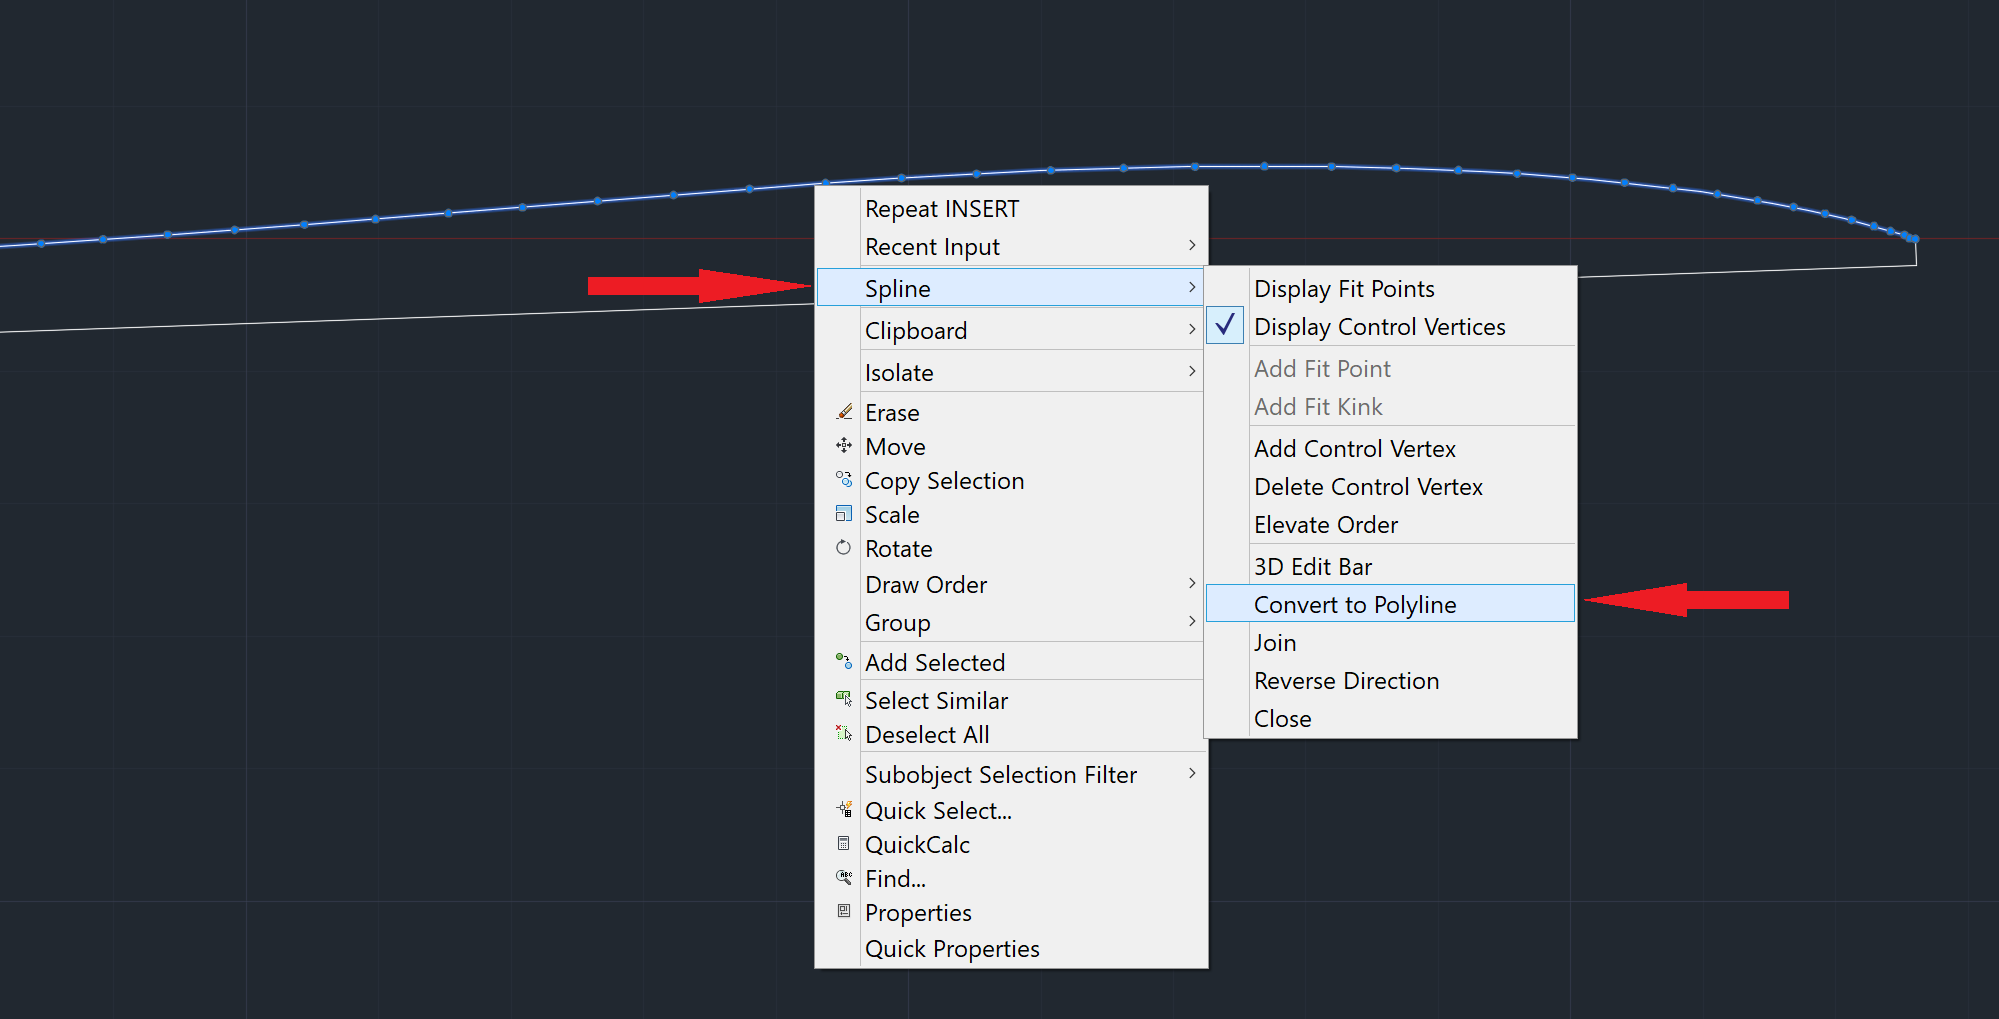
\includegraphics[width = 0.9\linewidth]{./Figures/general_shape/cad3.png}
		\caption{Convert Spline}
		\label{fig:cad3}
	\end{figure}
	\item Explode again (explode the polylines converted from spline).
	\item Rotate and delete overlapping lines if necessary.
	\item Select all lines and run ``eattext'' command, a window similar to fig~\ref{fig:cad4} should pop up, select ``Edit an existing data extraction'' then click the browse button.
	\begin{figure} [H]
		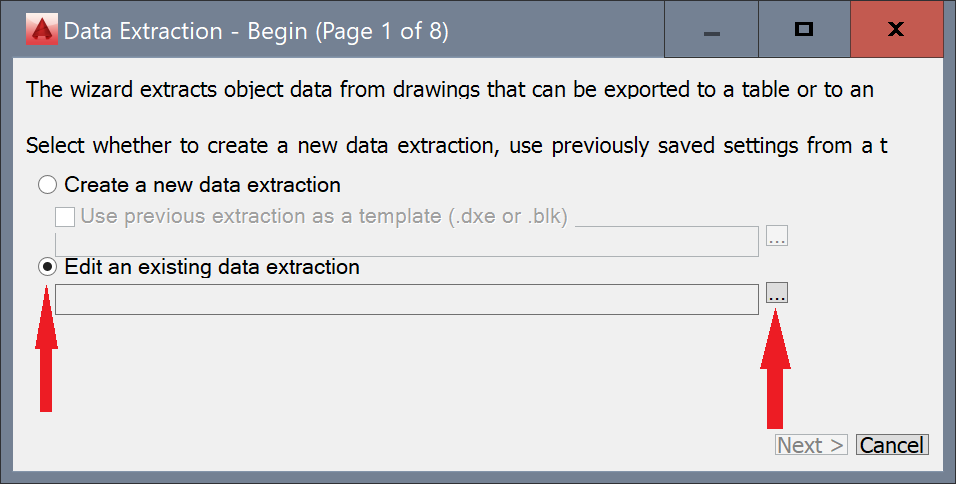
\includegraphics[width = 0.6\linewidth]{./Figures/general_shape/cad4.png}
		\caption{Eattext Page 1}
		\label{fig:cad4}
	\end{figure}
	\item Browse for the extraction templates, select the template with or without arc depending on the drawing. (The templates are included in the \textbf{``User Package.zip''} from \\ \href{https://github.com/ythuang96/FoamCutter}{https://github.com/ythuang96/FoamCutter})
	\begin{figure} [H]
		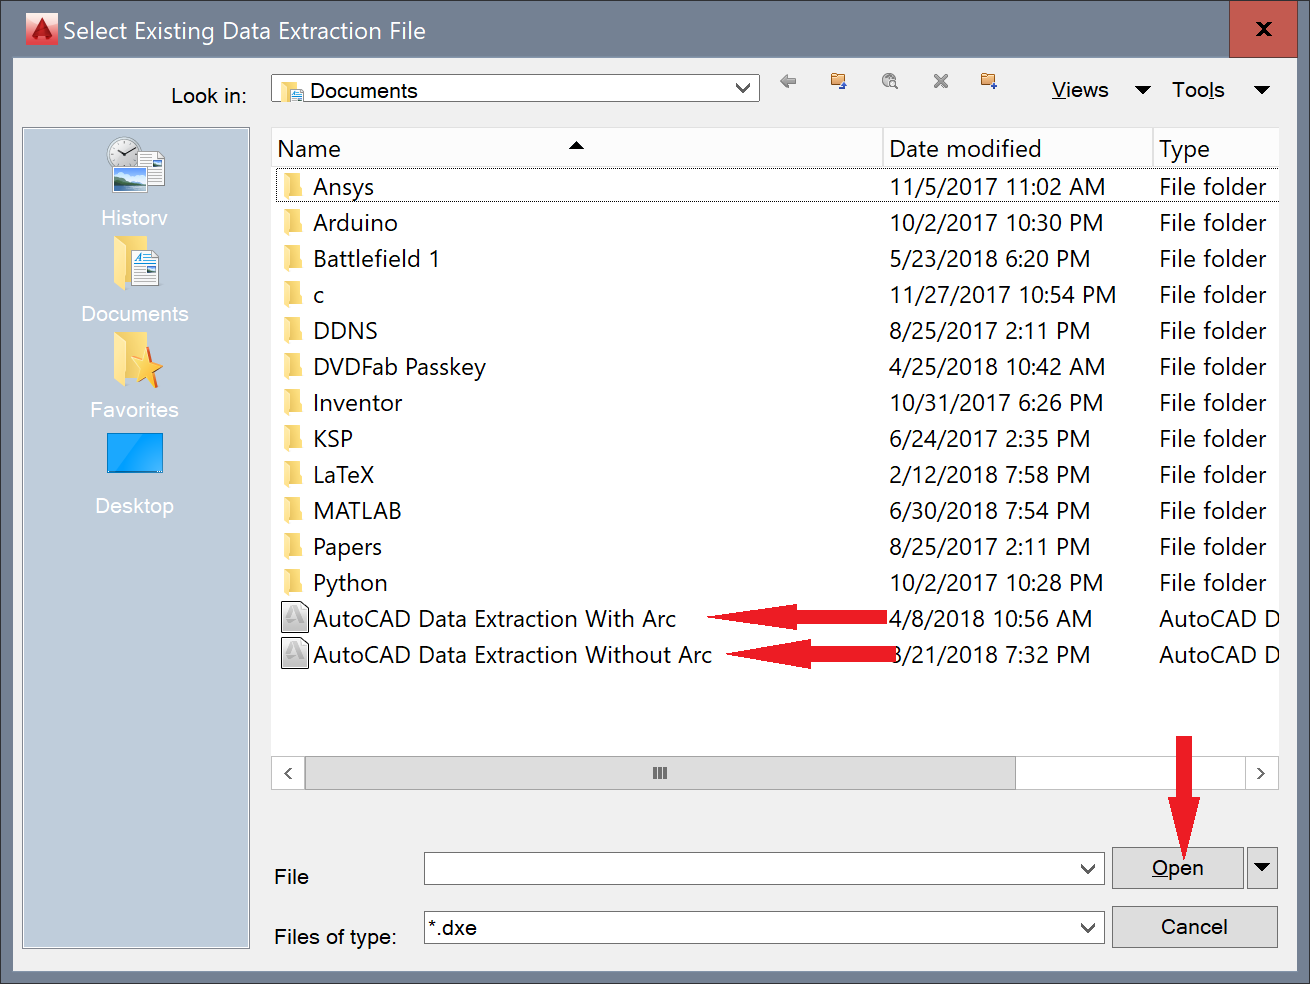
\includegraphics[width = 0.6\linewidth]{./Figures/general_shape/cad5.png}
		\caption{Browse for Data Extraction Templates}
		\label{fig:cad5}
	\end{figure}
	\item On page 2, check ``include current drawing'', select the one that is not the current drawing (if any) and click remove. 
	\begin{figure} [H]
		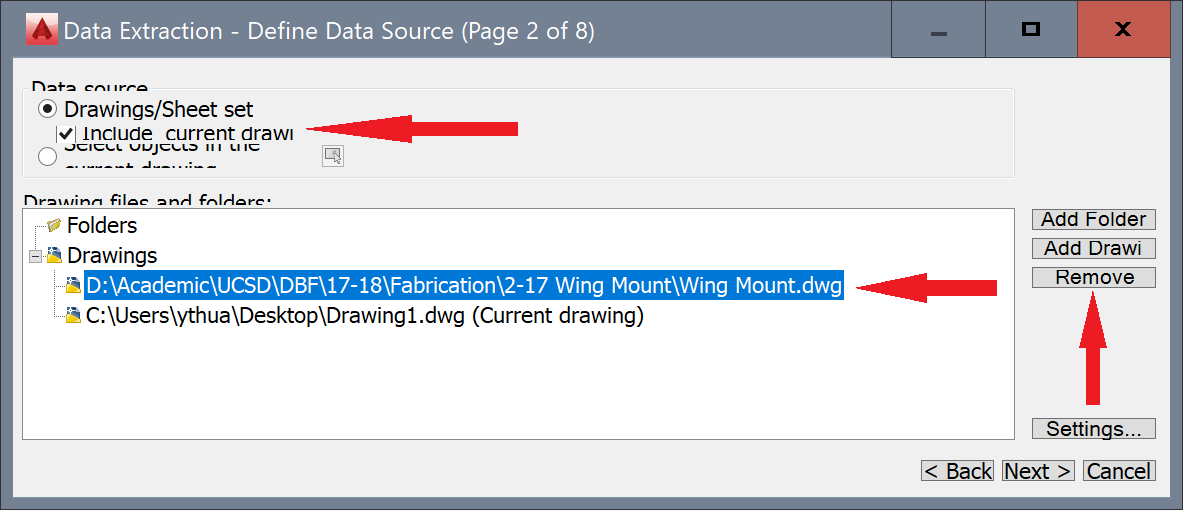
\includegraphics[width = 0.6\linewidth]{./Figures/general_shape/cad6.png}
		\caption{Eattext Page 2 Step 1}
	\end{figure}
	\item Then select the current drawing and click ``Next''.
	\begin{figure} [H]
		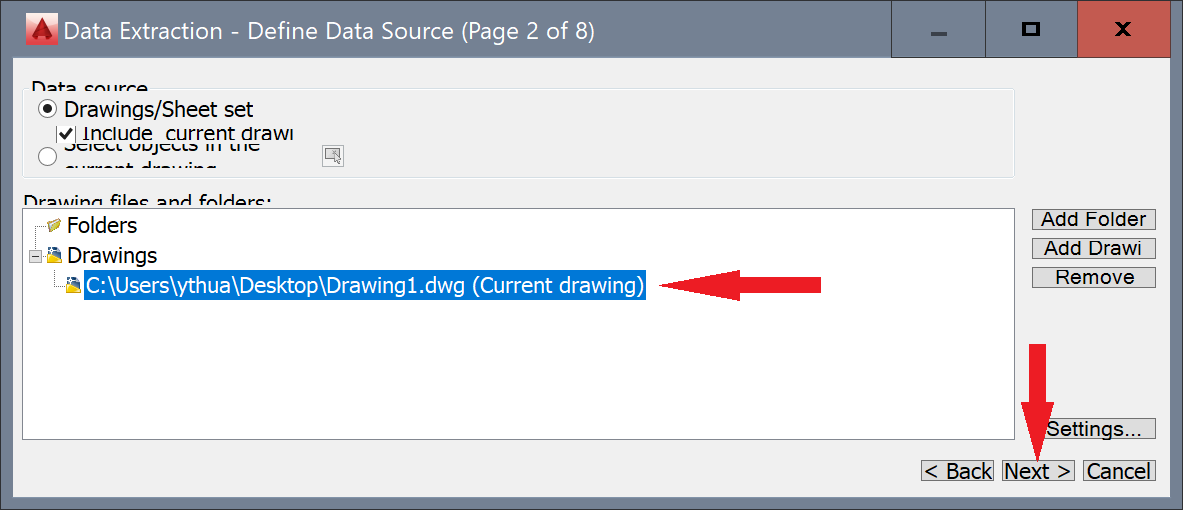
\includegraphics[width = 0.6\linewidth]{./Figures/general_shape/cad7.png}
		\caption{Eattext Page 2 Step 2}
	\end{figure}
	\item On page 3, make sure the drawing only has lines, or only has lines and arcs, depending on the template used. If not, cancel the process, fix the drawing, and redo the ``eattext'' command.
	\begin{figure} [H]
		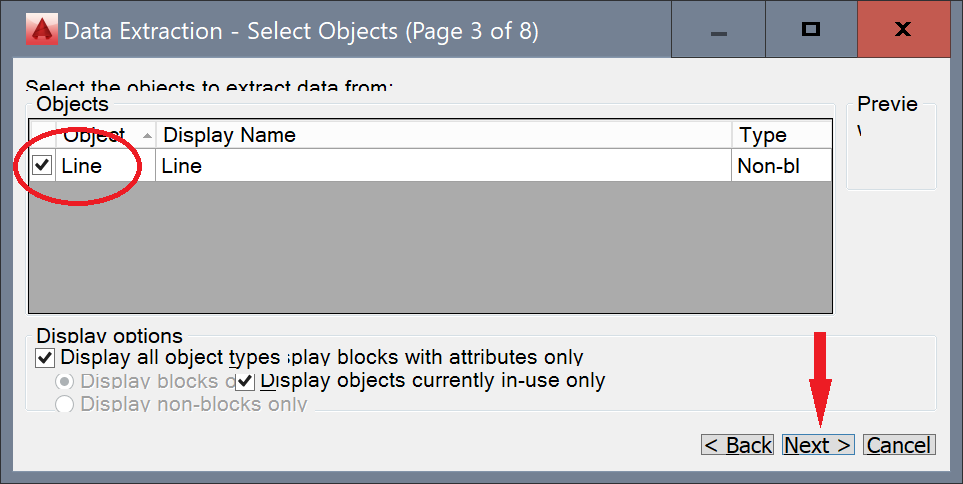
\includegraphics[width = 0.6\linewidth]{./Figures/general_shape/cad8.png}
		\caption{Eattext Page 3}
	\end{figure}
	
	\item Continue clicking ``Next'' until reaching page 6, name the data point file and save to the desired location. Click ``Next'' then ``Finish''.
	\begin{figure} [H]
		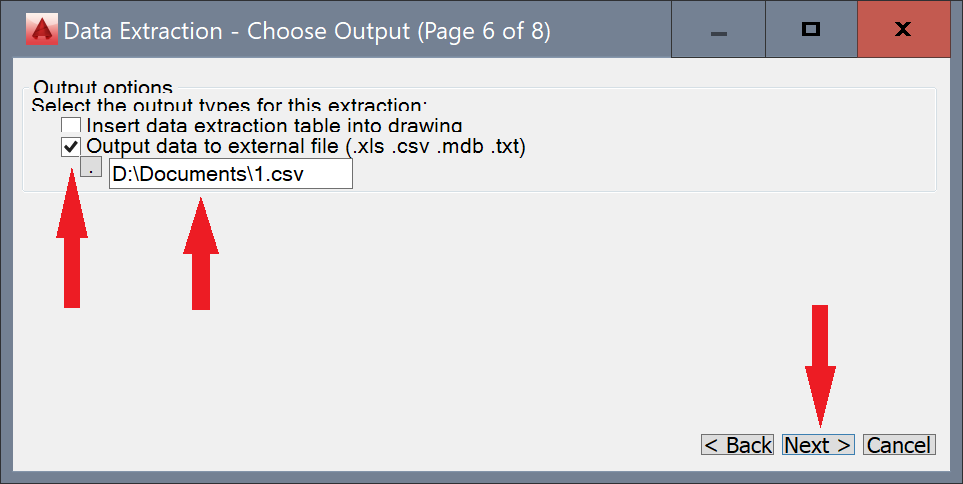
\includegraphics[width = 0.6\linewidth]{./Figures/general_shape/cad9.png}
		\caption{Eattext Page 6}
	\end{figure}
	
	\item Put the .csv file from AutoCAD into the same folder as the MatLAB script \\ \textbf{``DBF\_foamcutter\_general\_shape.m''} (provided in the \textbf{``User Package.zip''} from \\ \href{https://github.com/ythuang96/FoamCutter}{https://github.com/ythuang96/FoamCutter}) and run the MatLAB code. Follow the prompts, and the G-code should be ready.
	
	
\end{enumerate}

\newpage




\newpage
\chapter{Operate the FoamCutter}
\section{Switches}
The foamcutter has 3 switches installed as shown in fig~\ref{fig:switch} below.
\begin{figure} [H]
	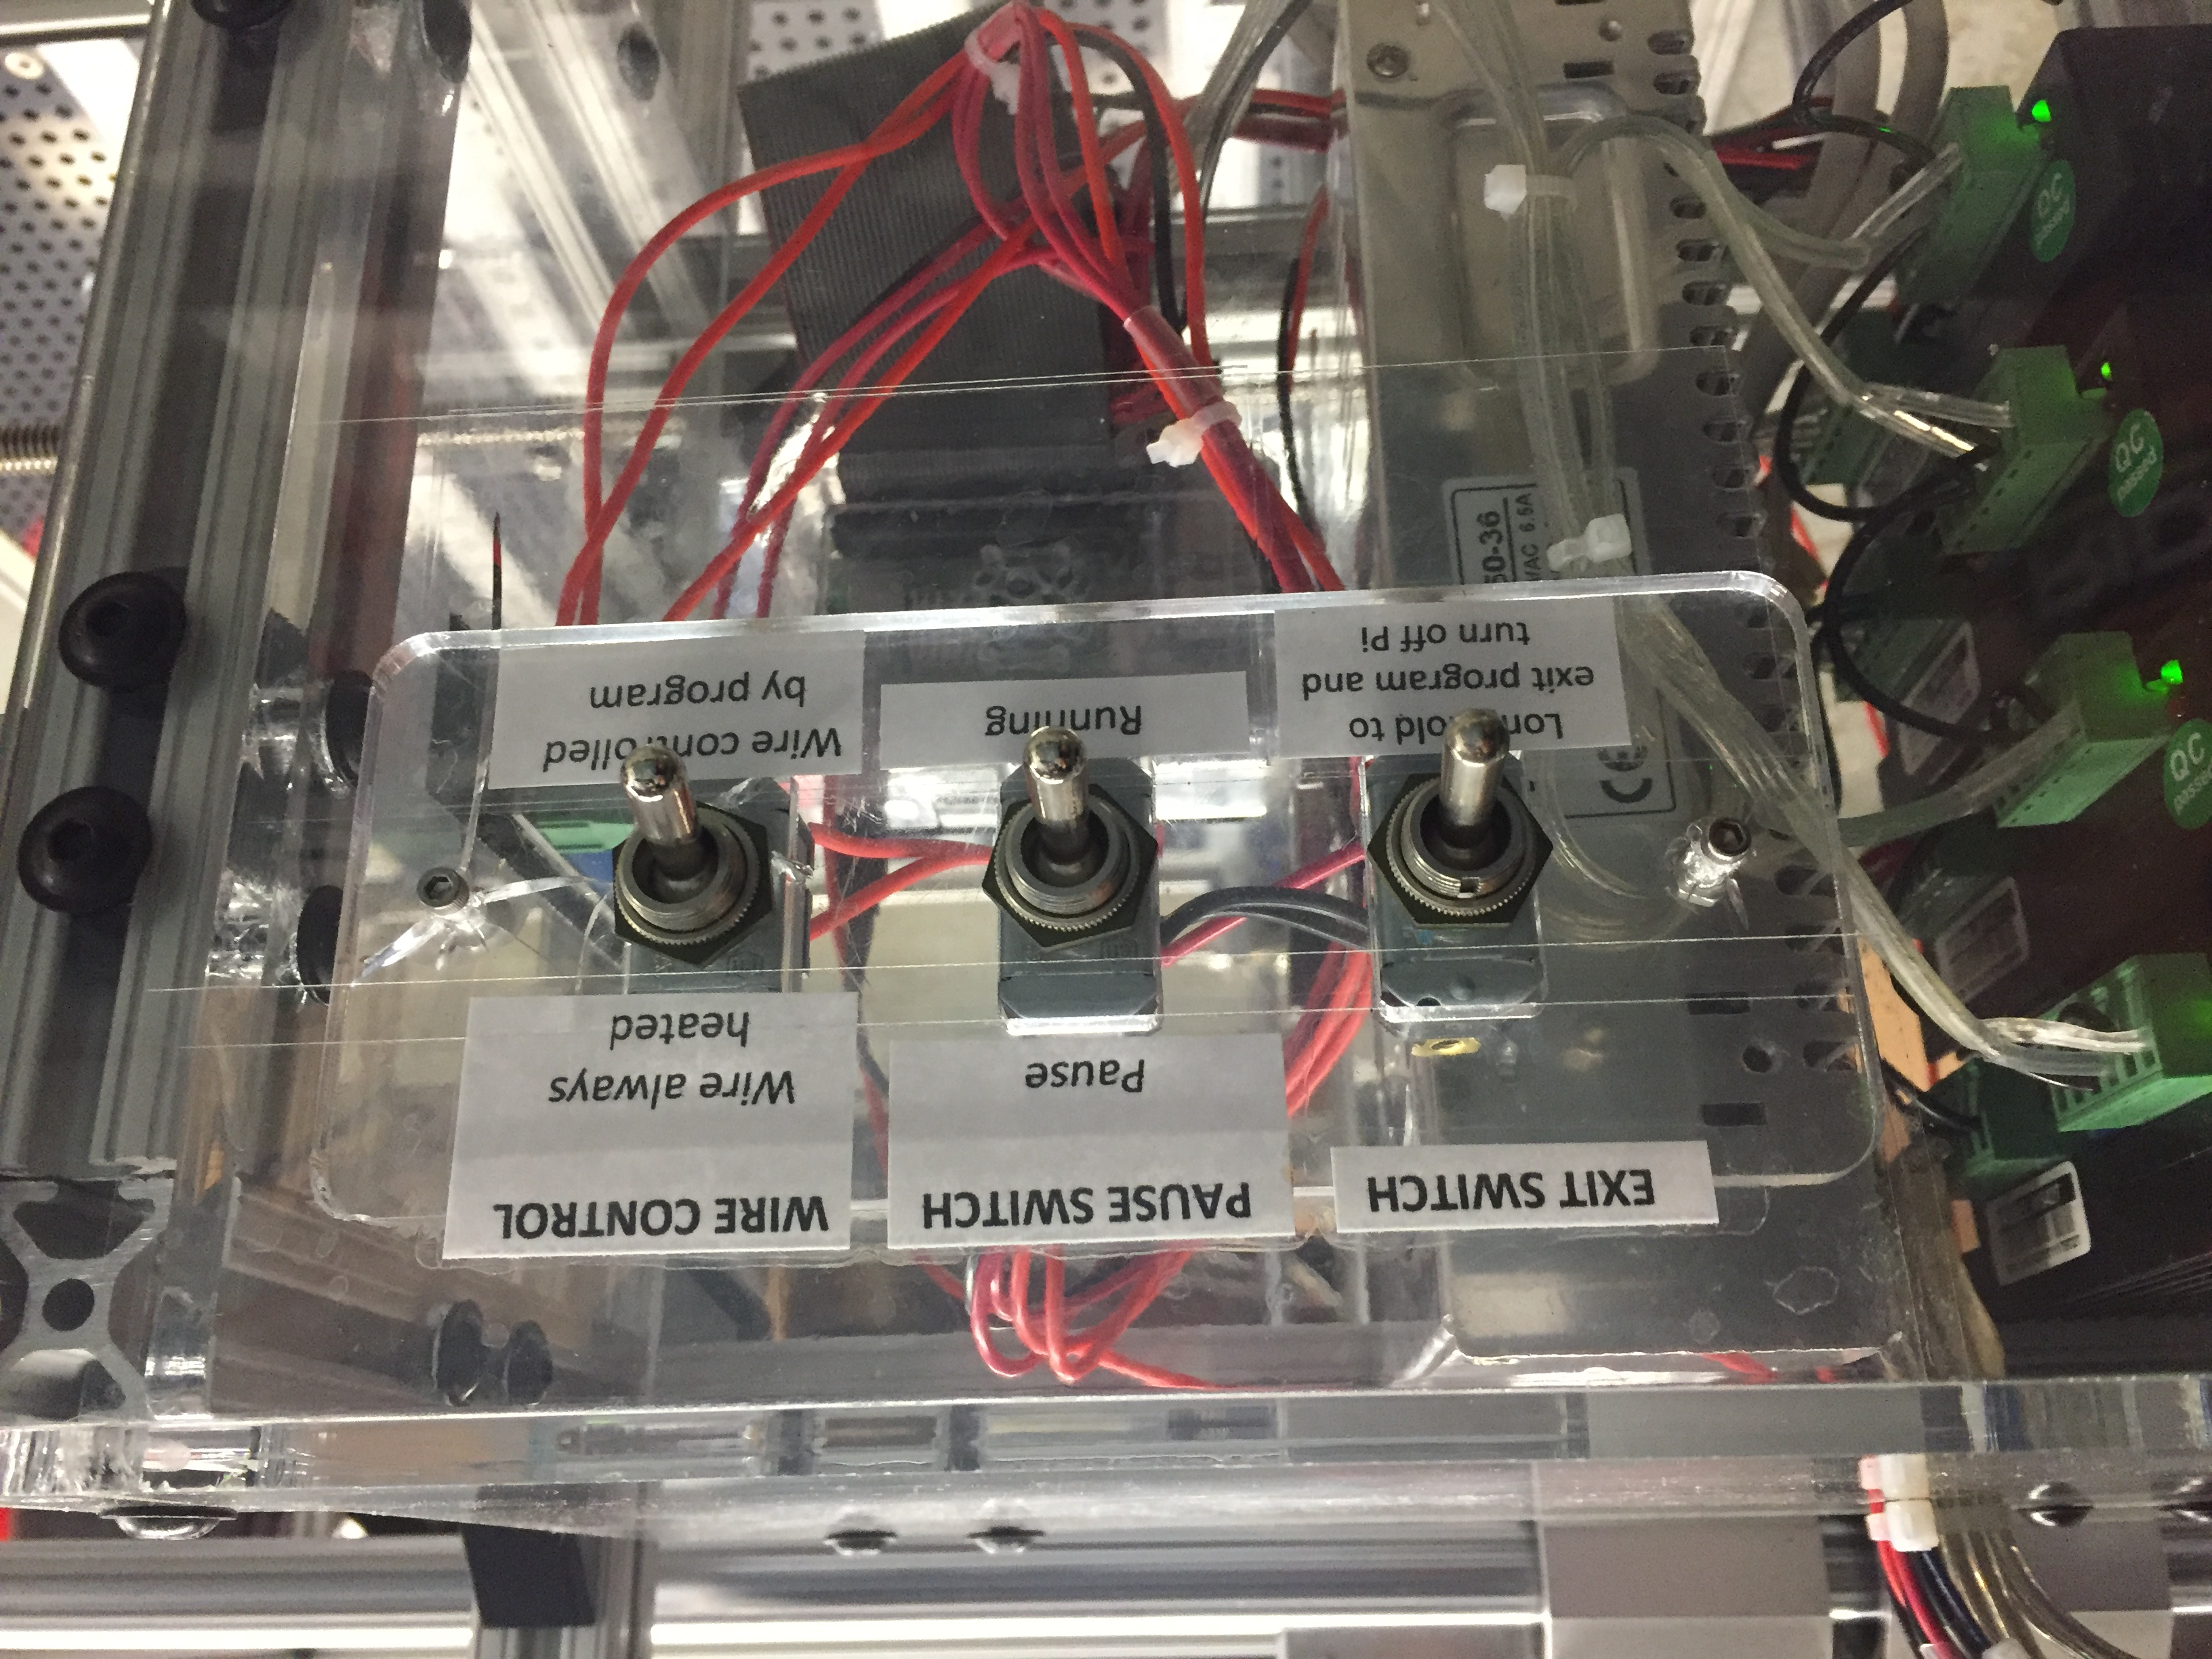
\includegraphics[width = 0.8\linewidth]{./Figures/electric.jpg}
	\caption{Three Switches of the Foamcutter}
	\label{fig:switch}
\end{figure}
\begin{itemize}[itemsep = 5pt,topsep=0pt]
	\item Left most switch: \textbf{Exit switch} \\
	Only operational when the foamcutter software is running. \\\
	Hold the switch for 4 seconds will stop all motor movement, exit the foamcutter software and shutdown the Raspberry Pi.
	\item Middle switch: \textbf{Pause switch}\\
	Only operational when the foamcutter software is running.\
	Toggle the switch up to pause the motor movements. \\
	Toggle the switch down to resume the motor movements.
	\item Right most switch: \textbf{Wire Control switch}\\
	Operational regardless of foamcutter software.\\
	Toggle the switch up will enable the wire heating when the wire power supply is turned on and connected.\\
	Toggle the switch down will enable the foamcutter software to control the wire heating. The software automatically turns on the wire heating when starting the cut and turns off the wire heating when cut ends. \textbf{This switch should generally be left at the down position for safety.}
\end{itemize}


\section{Start a Cut}
Please follow the steps below to operate the foamcutter:
\begin{enumerate}[itemsep = 5pt,topsep=0pt]
	\item Prepare the G-code following guide from Chapter 1 Section~\ref{sec:gcode}.
	\item Assemble the foamcutter following guide from Chapter 1 Section~\ref{sec:assemble}.
	\item Check that the Wire Control switch (right most switch) is toggled to the down position.
	\item Plug in the power cord.
	\item Plug in the power supply for the hot wire but do not turn it on.
	\item On your laptop, connect to the WiFi network named \textbf{``foamcutter''}, with password \textbf{``ucsdaiaadbf}
	\item Open PuTTY and connect to the Pi with user name \textbf{``pi''} and password \\ \textbf{``ucsdaiaadbf''}.
	\item Open WinSCP and connect to the Pi. Upload the G-code file to the Pi folder \\ \textbf{``/home/pi''}.
	\item In PuTTY, run: \textbf{sudo foamcutter}
	\item The software will first check the Pause switch status and will prompt to toggle the switch down if needed.
	\item The software will then ask to perform the homing process. Double check that the Molex connectors are connected, then press enter to perform homing. 
	\item The software will then enter the main menu, follow the prompts to select desired options to perform cuts or move the wire.
\end{enumerate}

\section{Secure the Foam}
The foam can be secured with acrylic plates with thumb screws on the three sides. Follow the steps below to secure the foam on the work panel:
\begin{enumerate}[itemsep = 5pt,topsep=0pt]
	\item Measure the width of the foam that need to be cut.
	\item Set one acrylic plate half of the width of the foam so that the foam will be centered on the work panel. Make sure both ruler reads the same so that the acrylic plate is in the vertical direction as shown in fig~\ref{fig:foam1} below.
	\begin{figure} [H]
		\includegraphics[width = 0.45\linewidth]{./Figures/secure_foam/1.jpg}
		\caption{Secure the Foam Step 2}
		\label{fig:foam1}
	\end{figure}
	\item Secure the first plate with 3 thumb screws. \textbf{Do not over tighten the thumbscrews, or the threads on the work panel might be destroyed.}
	\item Place the foam on the work panel with one side firmly against the guiding block and another side firmly against the first acrylic plate.
	\item Place a second acrylic plate firmly against the foam and secure with 3 thumb screws as shown in fig~\ref{fig:foam2} below.
	\begin{figure} [H]
		\includegraphics[width = 0.6\linewidth]{./Figures/secure_foam/2.jpg}
		\caption{Secure the Foam Step 5}
		\label{fig:foam2}
	\end{figure}
	\item Secure the back of the foam with another acrylic plate and secure with 3 thumb screws as shown in fig~\ref{fig:foam3} below.
	\begin{figure} [H]
		\includegraphics[width = 0.6\linewidth]{./Figures/secure_foam/3.jpg}
		\caption{Secure the Foam Step 6}
		\label{fig:foam3}
	\end{figure}
	\item Place a small piece of aluminum block on top of the foam to prevent vertical movement as shown in fig~\ref{fig:foam4} below.
	\begin{figure} [H]
		\includegraphics[width = 0.6\linewidth]{./Figures/secure_foam/4.jpg}
		\caption{Secure the Foam Step 7}
		\label{fig:foam4}
	\end{figure}
	\item To secure very small pieces of foam, one of the acrylic plates can be flipped as shown in fig~\ref{fig:foam5} below.
	\begin{figure} [H]
		\includegraphics[width = 0.6\linewidth]{./Figures/secure_foam/5.jpg}
		\caption{Secure the Foam Step 6}
		\label{fig:foam5}
	\end{figure}
\end{enumerate}

\section{End a Cut}
To the cutting operation half way through a G-code:
\begin{itemize}[itemsep = 5pt,topsep=0pt]
	\item In the PuTTY session, press \textbf{``Control + C''}. This will stop the cut and exit the program. It will also ask if desired to shutdown the Pi immediately.
	\item Or hold the Exit switch for more than 3 seconds. This will stop the cut and exit the program, but will also immediately shutdown the Pi.
\end{itemize}

To exit the program after the cut is finished, apart form the two options listed above, the user can also select the menu options to return to the main menu, and select the third option to exit the program. It will also ask if desired to shutdown the Pi immediately.

\section{Cleaning Up}
After the Pi is properly turned off by:
\begin{itemize}[itemsep = 5pt,topsep=0pt]
	\item Press Enter when seeing \textbf{``If you would like to shutdown the Pi now. Please press ENTER. Otherwise, press 'n' then press ENTER:''} when exiting the foamcutter software.
	\item Or run \textbf{``sudo shutdown now''} in PuTTY.
\end{itemize}
the green LED should flash a couple of times indicating the operating system is reading/writing to the SD card. After the green LED turns off, unplug the power cord and wrap it around the acrylic electronics box. Also remember to turn off the power supply for the hot wire and wrap the power cables for the hot wire around the two screws. 


\newpage
\chapter{Raspberry Pi Setup}
\begin{tcolorbox}
	{\large
		Note: \\
		All steps in this chapter are already performed on the currently used Raspberry Pi, and do not need to be performed again unless the Raspberry Pi or the SD card is damaged and needs replacement. 
	}
\end{tcolorbox}

\section{Install Raspbian on the Raspberry Pi}
Raspbian is one of the recommended operating system for the Raspberry Pi. The following steps are used to install Raspbian and setup the Pi.

\begin{enumerate}[itemsep = 5pt,topsep=0pt]
	\item Perform the Laptop setup guide in Chapter 1 Section~\ref{sec:laptop} if not already completed.
	\item Download the Raspbian Sketch Lite version at: \\ \href{https://www.raspberrypi.org/downloads/raspbian/}{https://www.raspberrypi.org/downloads/raspbian/} The Lite version does not have desktop support, but should be sufficient for the foamcutter.
	\item Download and install Etcher at \href{https://etcher.io/}{https://etcher.io/}.
	\item Plug in the SD card into a laptop and run Etcher.
	\item In Etcher, select the raspbian image just downloaded, then select the SD card. Lastly, click flash.
	\item Wait for flash to complete, the SD card should now have two partition with one named ``boot''.
	\item Enable SSH on the Pi by creating a file name ``ssh'' \textbf{without any extension} in the partition named ``boot'' on the SD card.
	\item Unplug the SD card from the laptop and plug into the Pi. Connect a Ethernet cable from the Pi to same router your laptop is currently connected to.
	\item Connect power to the Pi.
	\item SSH into the Pi by opening up PuTTY and create a new session with host name: \textbf{``raspberrypi.local''}. Note on using PuTTY: to copy text from PuTTY, simply select the text, do not press ``Control + C''. To paste text to PuTTY, simply right click mouse, do not press ``Control + V''.
	\item Enter the user name \textbf{``pi''} then password \textbf{``raspberry''}.
	\item Change the log in password: enter \textbf{``passwd''} on the command line and press Enter. Enter the current password \textbf{``raspberry''}, then enter the new password \textbf{``ucsdaiaadbf''} twice.
	\item Change the name of the Pi by entering \textbf{``sudo raspi-config''}, select \textbf{``Network Options $\rightarrow$ Hostname''}, then enter the new hostname: \textbf{``foamcutter''}, then press Enter.
	\item Select ``Finish'', then press Enter. When asked to reboot, select ``Yes''.
\end{enumerate}

\section{Install WiringPi on the Raspberry Pi}
WiringPi is a GPIO Interface library written for the Raspberry Pi. A complete guide can be found at: \href{http://wiringpi.com/}{http://wiringpi.com/}. To install on the pi, follow the complete guide at: \href{http://wiringpi.com/download-and-install/}{http://wiringpi.com/download-and-install/} or follow the steps below:

\begin{enumerate}[itemsep = 5pt,topsep=0pt]
	\item Power on the Pi and open PuTTY on your laptop.
	\item Double click on the saved PuTTY session named ``foamcutter'' as shown in fig~\ref{fig:wiringpi} below.
	\begin{figure} [H]
	\includegraphics[width = 0.6\linewidth]{./Figures/Laptop_Setup/putty3.png}
	\caption{SSH to the Raspberry Pi}
	\label{fig:wiringpi}
	\end{figure}
	\item Enter user name \textbf{``pi''} and password \textbf{``ucsdaiaadbf''}.
	\item Update the operating system using the following two command:
	\begin{itemize}[noitemsep,topsep=0pt]
		\item \textbf{sudo apt-get update}
		\item \textbf{sudo apt-get upgrade}
	\end{itemize}
	\item Install GIT using:
	\begin{itemize}[noitemsep,topsep=0pt]
		\item \textbf{sudo apt-get install git-core}
	\end{itemize}
	\item Install WiringPi using:
	\begin{itemize}[noitemsep,topsep=0pt]
		\item \textbf{cd}
		\item \textbf{git clone git://git.drogon.net/wiringPi}
		\item \textbf{cd ~/wiringPi}
		\item \textbf{./build}
	\end{itemize}
	\item Completed when seeing: \\
	
\textbf{All Done}. \\
	
	\textbf{NOTE: To compile programs with wiringPi, you need to add: \\
	-lwiringPi \\
	to your compile line(s) To use the Gertboard, MaxDetect, etc.\\
	code (the devLib), you need to also add:\\
	-lwiringPiDev\\
	to your compile line(s).\\}
	
\end{enumerate}

\section{Making the Pi into a Wireless Hotspot}
Making the Pi into a Wireless Hotspot will enable operation of the foamcutter even in areas without a wireless network. The following steps are adapted from: \href{https://elinux.org/RPI-Wireless-Hotspot}{https://elinux.org/RPI-Wireless-Hotspot}

\begin{enumerate}[itemsep = 5pt,topsep=0pt]
	\item SSH into the Pi via PuTTY.
	\item Run: \textbf{sudo apt-get install hostapd udhcpd}
	\item Run: \textbf{sudo nano /etc/udhcpd.conf} This will open a text editor, use keyboard instead of mouse to navigate.
		\begin{itemize}[noitemsep,topsep=0pt]
			\item Find the line starting with \textbf{interface} and change to \textbf{interface wlan0}
			\item Find the line starting with \textbf{opt router} and change to \textbf{opt router 192.168.42.1}
			\item Press \textbf{Control + O} then \textbf{Enter} then \textbf{Control + X} to save and close file.
		\end{itemize}
	
	\item Run: \textbf{sudo nano /etc/default/udhcpd}
	\begin{itemize}[noitemsep,topsep=0pt]
		\item Add \textbf{\#} to the front of the line \textbf{DHCPD\_ENABLED="no"}
		\item Press \textbf{Control + O} then \textbf{Enter} then \textbf{Control + X} to save and close file.
	\end{itemize}

	\item Run: \textbf{sudo ifconfig wlan0 192.168.42.1}
	\item Run: \textbf{sudo nano /etc/network/interfaces}
	\begin{itemize}[noitemsep,topsep=0pt]
		\item Add the following lines to the bottom of the file if the line \textbf{iface wlan0 inet dhcp} is not present, otherwise replace it: \\
		\textbf{iface wlan0 inet static} \\
		\textbf{address 192.168.42.1} \\
		\textbf{netmask 255.255.255.0}
		\item Add \textbf{\#} to the beginning of each of the following lines if present: \\
		\textbf{allow-hotplug wlan0}\\
		\textbf{wpa-roam /etc/wpa\_supplicant/wpa\_supplicant.conf}\\
		\textbf{iface default inet manual}
		\item Press \textbf{Control + O} then \textbf{Enter} then \textbf{Control + X} to save and close file.
	\end{itemize}

	\item Run: \textbf{sudo nano /etc/hostapd/hostapd.conf}
	\begin{itemize}[noitemsep,topsep=0pt]
		\item Add the following lines to the bottom of the file:\\
		\textbf{interface=wlan0} \\
		\textbf{driver=nl80211}\\
		\textbf{ssid=foamcutter}\\
		\textbf{hw\_mode=g}\\
		\textbf{channel=6}\\
		\textbf{macaddr\_acl=0}\\
		\textbf{auth\_algs=1}\\
		\textbf{ignore\_broadcast\_ssid=0}\\
		\textbf{wpa=2}\\
		\textbf{wpa\_passphrase=ucsdaiaadbf}\\
		\textbf{wpa\_key\_mgmt=WPA-PSK} \\   
		\textbf{rsn\_pairwise=CCMP}\\
		
		\textbf{channel=1}\\
		\textbf{ieee80211n=1}    \\     
		\textbf{wmm\_enabled=1}    \\ 
		\textbf{ht\_capab=[HT40+][SHORT-GI-20][DSSS\_CCK-40]}
		\item Press \textbf{Control + O} then \textbf{Enter} then \textbf{Control + X} to save and close file.
	\end{itemize}

	\item Run: \textbf{sudo nano /etc/default/hostapd}
	\begin{itemize}[noitemsep,topsep=0pt]
		\item Change the line from \textbf{\#DAEMON\_CONF=""} to \\ \textbf{DAEMON\_CONF="/etc/hostapd/hostapd.conf"}
		\item Press \textbf{Control + O} then \textbf{Enter} then \textbf{Control + X} to save and close file.
	\end{itemize}

	\item Run: \textbf{sudo nano /etc/default/hostapd}
	\begin{itemize}[noitemsep,topsep=0pt]
		\item Add \textbf{net.ipv4.ip\_forward=1} to the bottom of the file.
		\item Press \textbf{Control + O} then \textbf{Enter} then \textbf{Control + X} to save and close file.
	\end{itemize}

	\item Run: \textbf{sudo update-rc.d hostapd enable}
	\item Run: \textbf{sudo update-rc.d udhcpd enable}
	\item Run: \textbf{sudo reboot}	
\end{enumerate}


\newpage
\begin{appendices}
\chapter{C Code for the Foamcutter Program}
\section{foamcutter.c}
The C code for the foamcutter program, \textbf{foamcutter.c} is attached below. Verison 1.0.0, lasted updated: 6/30/2018.
\includepdf[pages=-, pagecommand={},landscape=false]{../Code/C/foamcutter.pdf}

\section{foamcutter\_setup.h}
The setting file, \textbf{foamcutter\_setup.h} is attached below. 
\includepdf[pages=-, pagecommand={},landscape=false]{../Code/C/foamcutter_setup.pdf}

\chapter{MatLab Code for G-code Generation}
\section{DBF\_foamcutter\_general\_shape.m}
The MatLab code for generating G-code for general shape, \\ \textbf{DBF\_foamcutter\_general\_shape.m} is attached below. Last updated: 8/26/2018.
\includepdf[pages=-, pagecommand={},landscape=false]{../Code/MatLab/DBF_foamcutter_general_shape.pdf}

\section{DBF\_foamcutter\_wing.m}
The MatLab code for generating G-code for wing, \textbf{DBF\_foamcutter\_wing.m} is attached below. Last updated: 8/23/2018.
\includepdf[pages=-, pagecommand={},landscape=false]{../Code/MatLab/DBF_foamcutter_wing.pdf}

\chapter{Drawings}
The complete SolidWorks drawings can be found at \\ \href{https://github.com/ythuang96/FoamCutter}{https://github.com/ythuang96/FoamCutter}. The following is the complete assembly in SolidWorks:
 \begin{figure} [H]
 	\includegraphics[width = 0.9\linewidth]{./Figures/SW.png}
 \end{figure}

Drawings attached below are all aluminum pieces that required machining. But the drawings are not drawn in compliance with engineering standards and therefore should only be used as a reference when machining yourself. 
\includepdf[pages=-, pagecommand={},landscape=true]{1.pdf}

\chapter{Part List}
The parts used for this project are listed below.
\includepdf[pages=-, pagecommand={},landscape=true]{../Parts/Part_List.pdf}

\chapter{Purchase History}
The purchase history of this project are listed below.
\includepdf[pages=-, pagecommand={},landscape=true]{../Parts/Purchase_History.pdf}



\end{appendices}
\end{document}
